\chapter{PENGUJIAN DAN ANALISIS}
\label{chap:pengujiananalisis}

% Ubah bagian-bagian berikut dengan isi dari pengujian dan analisis

Pada bab ini akan dipaparkan skenario pengujian yang  dilakukan berdasarkan dari metodol\\ogi yang telah dibahas sebelumnya beserta dengan pembahasannya. Pengujian akan dilaksanakan untuk menjawab permasalahan yang diangkat sehingga dapat ditarik kesimpulan dari pelaksanaan tugas akhir ini.

\section{Skenario Pengujian}
\label{sec:skenariopengujian}

Pengujian ini akan dilakukan dengan menggunakan Intel NUC 11 Performance Kit yang telah terhubung ke internet untuk mengakses program melalui browser. Dibutuhkan juga tambahan koneksi dengan webcam eksternal sebagai media pengambilan data yang akan diproses pada program, serta keyboard, mouse, dan monitor untuk memudahkan dalam mengoperasikan program. Adapun pengujian ini akan mengikuti beberapa skenario - skenario pengujian yang ditentukan sebagai berikut:


\begin{longtable}{|c|p{8cm}|p{6cm}|}
  \caption{Skenario Pengujian}
  \label{tb:skenario}                                   \\
  \hline
  \rowcolor[HTML]{C0C0C0}
  \textbf{No.} & \multicolumn{1}{>{\centering\arraybackslash}p{8cm}|}{\textbf{Skenario Pengujian}} & \multicolumn{1}{>{\centering\arraybackslash}p{6cm}|}{\textbf{Variasi Pengujian}} \\ \hline
  1 & Skenario pengujian berdasarkan bentuk model  & 3 model yang berbeda \\ \hline
  2 & Skenario pengujian berdasarkan kondisi pencahayaan yang berbeda & Intensitas cahaya 35 lux, 80 lux, 125 lux \\ \hline
  3 & Skenario pengujian berdasarkan jarak subjek yang berbeda & Jarak 180 cm, 240 cm, 300 cm \\ \hline
  4 & Skenario pengujian dengan menggunakan subjek yang berbeda selain penulis & 1 subjek perempuan dan 1 subjek laki - laki \\ \hline
  5 & Skenario pengujian pembentukan kalimat dan konversi menjadi media suara & 3 kalimat yang dibentuk dari 3 kosakata dan 4 kalimat yang dibentuk dari 2 kosakata \\ \hline
\end{longtable} 

\section{Pengujian Bentuk Model}
\label{sec:analisismodel}

Pengujian bentuk model penerjemah bahasa isyarat Indonesia (BISINDO) dilakukan dengan melakukan perubahan struktur dari \emph{layer} yang digunakan, baik dari segi pemilihan tipe \emph{layer}, fungsi \emph{activation}, serta jumlah unit aktivasi yang digunakan. Pengujian ini didasari dari struktur model yang telah dibahas pada sub bab \ref{sec:metodologipose}. Serangkaian model yang diuji akan dilihat bagaimana performa hasil dari \emph{training} model, melalui grafik \emph{accuracy} dan \emph{loss} yang dihasilkan. Digunakan \emph{confusion matrix} untuk mengamati bagaimana hasil dari pengujian model terhadap serangkaian data gerakan bahasa isyarat dengan membandingkan hasil prediksi model dengan data aktual yang ada untuk masing - masing kosakata atau \emph{class} yang ada. Berdasarkan \emph{confusion matrix} ini juga dapat dihasilkan matrix evaluasi berupa \emph{accuracy}, \emph{precision}, \emph{recall}, dan \emph{F1-score}. Setiap model yang diuji menggunakan partisi data \emph{training} dan validasi yang sama, yaitu dengan perbandingan 70:30. Hal ini menunjukkan bahwa dari keseluruhan data yang digunakan, akan terdapat 70\% data \emph{training} dan 30\% data validasi. Untuk setiap kosakata yang digunakan sesuai dengan yang telah dijelaskan pada sub bab \ref{sec:metodologidataset}. Keseluruhan model akan dilatih sebanyak 12 \emph{epoch}. Pengujian ini bertujuan untuk melihat bagaimana perubahan struktur dari \emph{layer} akan berpengaruh pada performa model penerjemah yang dihasilkan.

\subsection{Model Pertama}
\label{sec:analisismodel1}
Model pertama menggunakan 2 buah \emph{layer} LSTM. \emph{Layer} LSTM pertama menggunakan fungsi aktivasi \emph{relu} dan dengan unit aktivasi bernilai 128 dan \emph{layer} LSTM kedua menggunakan fungsi aktivasi \emph{relu} dan dengan unit aktivasi bernilai 64. Untuk setiap \emph{layer} LSTM akan diikuti dengan \emph{layer} Dropout bernilai 0.5 untuk mencegah nilai \emph{weight} yang terlalu tinggi. Setelah serangkaian \emph{layer} LSTM, diikuti dengan \emph{layer} Dense dengan fungsi aktivasi \emph{relu} dan dengan unit aktivasi bernilai 32. Struktur lengkap dari model ini dapat dilihat pada \ref{fig:model1-struktur}.

\begin{figure}[H]
  \centering

  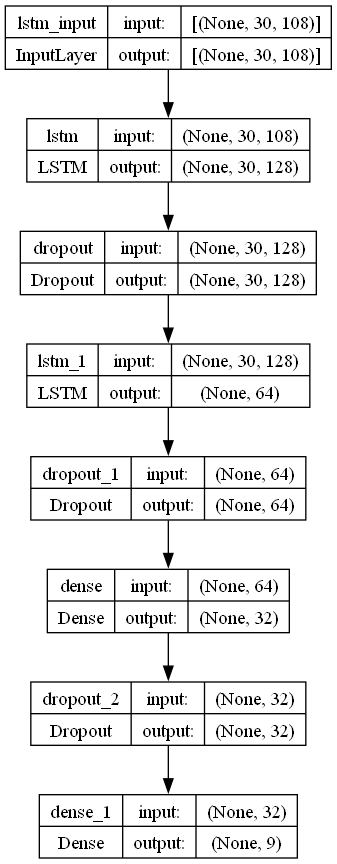
\includegraphics[scale=0.5]{gambar/bab4-uji-model-worst-model.png}

  \caption{Struktur model pertama}
  \label{fig:model1-struktur}
\end{figure}

Berdasarkan dari \emph{training} yang telah dilakukan didapatkan bahwa model menghasilkan akurasi validasi bernilai 0.89 dan akurasi \emph{training} bernilai 0.71. Data ini menunjukkan bahwa model memiliki akurasi yang cukup baik. Untuk nilai \emph{loss training} bernilai cukup tinggi, yaitu bernilai 2.81 dan \emph{loss} validasi bernilai 0.76 yang cukup rendanh jika dibandingkan dengan nilai \emph{loss training}. Nilai dari \emph{loss training} terlihat melonjak di \emph{epoch} terakhir, yaitu pada \emph{epoch} 12. Hal ini selaras dengan penurunan \emph{accuracy} model setelah \emph{epoch} 10. Grafik akurasi dan \emph{loss} dapat dilihat pada gambar \ref{fig:model1-train-acc} dan gambar \ref{fig:model1-train-loss}.

\begin{figure}[H]
  \centering

  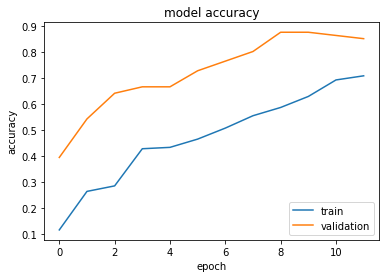
\includegraphics[scale=0.6]{gambar/bab4-uji-model-worst-acc.png}

  \caption{Hasil \emph{accuracy} model pertama}
  \label{fig:model1-train-acc}
\end{figure}

\begin{figure}[H]
  \centering

  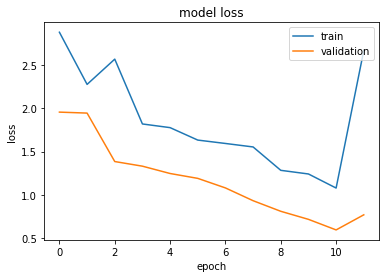
\includegraphics[scale=0.6]{gambar/bab4-uji-model-worst-loss.png}

  \caption{Hasil \emph{loss} model pertama}
  \label{fig:model1-train-loss}
\end{figure}

Kemudian berdasarkan model yang telah dihasilkan, dilakukan pengujian dengan dataset \emph{testing} yang menghasilkan \emph{confusion matrix}. Dapat dilihat pada gambar \ref{fig:model1-cf}, untuk kosakata "maaf", "tolong", "rumah", "delete", dan "translate" menghasilkan prediksi yang tepat untuk keseluruhan dataset \emph{testing} yang diujikan. Namun, kosakata "nama", "saya", "siapa", dan "standby" menghasilkan beberapa prediksi yang tidak sesuai dengan dataset \emph{testing}. Kosakata "nama" menghasilkan 6 prediksi tepat dan 4 prediksi yang kurang tepat (1 dataset \emph{testing} bernilai "siapa" dan 3 dataset \emph{testing} bernilai "rumah"). Kosakata "saya" menghasilkan 10 prediksi tepat dan 2 prediksi yang kurang tepat (dataset \emph{testing} bernilai "translate"). Kosakata "siapa" menghasilkan 3 prediksi tepat dan 5 prediksi yang kurang tepat (2 dataset \emph{testing} bernilai "tolong",  2 dataset \emph{testing} bernilai "saya", dan 1 dataset \emph{testing} bernilai "translate"). Kosakata "standby" menghasilkan 7 prediksi tepat dan 1 prediksi yang kurang tepat (dataset \emph{testing} bernilai "saya"). Adapun berdasarkan hasil \emph{confusion matrix} ini didapat matrix evaluasi berupa \emph{accuracy}, \emph{precision}, \emph{recall}, dan \emph{F1-score} yang dapat dilihat pada tabel \ref{tb:model1stat}. Rata - rata nilai \emph{accuracy} sebesar 0.85, rata - rata nilai \emph{precision} sebesar 0.85, rata - rata nilai \emph{recall} sebesar 0.85, dan rata - rata nilai \emph{F1-score} sebesar 0.83.

\begin{figure}[H]
  \centering

  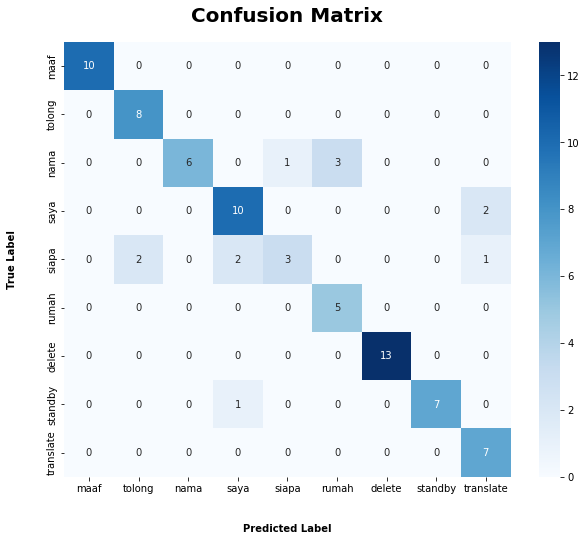
\includegraphics[scale=0.6]{gambar/bab4-uji-model-worst-cf.png}

  \caption{\emph{Confusion} model pertama}
  \label{fig:model1-cf}
\end{figure}

\begin{longtable}{|c|c|c|c|c|}
  \caption{Matrix Evaluasi Model 1}
  \label{tb:model1stat}                                   \\
  \hline
  \rowcolor[HTML]{C0C0C0}
  \textbf{Kosakata} & \textbf{\emph{Accuracy}} & \textbf{\emph{Precision}} & \textbf{\emph{Recall}} & \textbf{\emph{F1-Score}} \\
  \hline
  Maaf              & 1.00                     & 1.00                        & 1.00                   & 1.00                \\
  Tolong            & 1.00                     & 0.80                        & 1.00                   & 0.89                \\
  Nama              & 0.60                     & 1.00                        & 0.60                   & 0.75                \\
  Saya              & 0.83                     & 0.77                        & 0.83                   & 0.80                \\
  Siapa             & 0.37                     & 0.75                        & 0.38                   & 0.50                \\
  Rumah             & 1.00                     & 0.62                        & 1.00                   & 0.77                \\
  Delete            & 1.00                     & 1.00                        & 1.00                   & 1.00                \\
  Standby           & 0.87                     & 1.00                        & 0.88                   & 0.93                \\
  Translate         & 1.00                     & 0.70                        & 1.00                   & 0.82                \\
  \hline
\end{longtable}

\subsection{Model Kedua}
\label{sec:analisismodel2}

Model kedua diawali dengan \emph{layer} \textit{TimeDistributed} yang di dalamnya terdapat \emph{layer} \textit{Dense} dengan fungsi aktivasi '\textit{tanh}' dan unit aktivasi bernilai 128. Kemudian dilanjutkan dengan 1 buah \emph{layer} LSTM yang menggunakan fungsi aktivasi \emph{tanh} dan dengan unit aktivasi bernilai 64. \emph{Layer} LSTM akan diikuti dengan \emph{layer} Dropout bernilai 0.5 untuk mencegah nilai \emph{weight} yang terlalu tinggi. Setelah serangkaian \emph{layer} LSTM, diikuti dengan \emph{layer} Dense dengan fungsi aktivasi \emph{relu} dan dengan unit aktivasi bernilai 32. Struktur lengkap dari model ini dapat dilihat pada \ref{fig:model2-struktur}.

\begin{figure}[H]
  \centering

  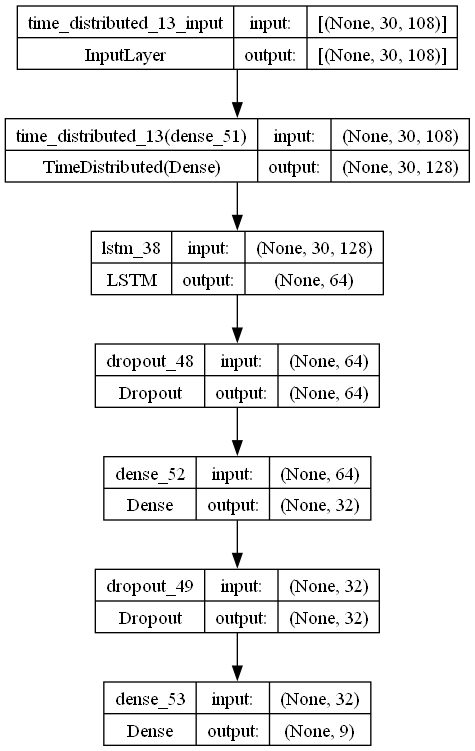
\includegraphics[scale=0.6]{gambar/bab4-uji-model-second-model.png}

  \caption{Struktur model kedua}
  \label{fig:model2-struktur}
\end{figure}

Berdasarkan dari \emph{training} yang telah dilakukan didapatkan bahwa model menghasilkan akurasi \emph{training} bernilai 0.96 dan akurasi validasi bernilai 0.93. Data ini menunjukkan bahwa model memiliki akurasi yang baik. Terdapat penurunan pada akurasi validasi pada \emph{epoch} terakhir, tetapi kebalikannya untuk akurasi \emph{training} mengalami kenaikan melebihi akurasi validasi. Untuk nilai \emph{loss training} bernilai 0.32 dan \emph{loss} validasi bernilai 0.25 yang cukup rendah jika dibandingkan dengan nilai \emph{loss training}. Data ini menunjukkan bahwa model memiliki \emph{error} prediksi yang kecil. Grafik akurasi dan \emph{loss} dapat dilihat pada gambar \ref{fig:model2-train-acc} dan gambar \ref{fig:model2-train-loss}.

\begin{figure}[H]
  \centering

  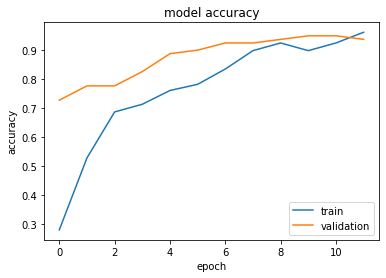
\includegraphics[scale=0.6]{gambar/bab4-uji-model-second-acc.png}

  \caption{Hasil \emph{accuracy} model kedua}
  \label{fig:model2-train-acc}
\end{figure}

\begin{figure}[H]
  \centering

  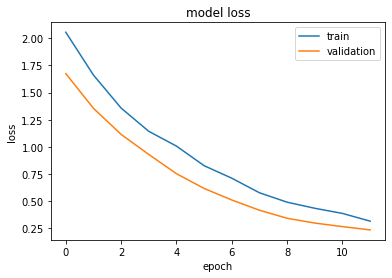
\includegraphics[scale=0.6]{gambar/bab4-uji-model-second-loss.png}

  \caption{Hasil \emph{loss} model kedua}
  \label{fig:model2-train-loss}
\end{figure}


Kemudian berdasarkan model yang telah dihasilkan, dilakukan pengujian dengan dataset \emph{testing} yang menghasilkan \emph{confusion matrix}. Dapat dilihat pada gambar \ref{fig:model2-cf}, untuk kosakata "tolong", "nama", "rumah", "delete", dan "translate" menghasilkan prediksi yang tepat untuk keseluruhan dataset \emph{testing} yang diujikan. Namun, kosakata "saya", "siapa", dan "standby" menghasilkan beberapa prediksi yang tidak sesuai dengan dataset \emph{testing}. Kosakata "maaf" menghasilkan 10 prediksi tepat dan 1 prediksi yang kurang tepat (dataset \emph{testing} bernilai "standb\\y"). Kosakata "saya" menghasilkan 11 prediksi tepat dan 2 prediksi yang kurang tepat (dataset \emph{testing} bernilai "siapa"). Kosakata "siapa" menghasilkan 5 prediksi tepat dan 1 prediksi yang kurang tepat (dataset \emph{testing} bernilai "saya"). Kosakata "standby" menghasilkan 7 prediksi tepat dan 1 prediksi yang kurang tepat (dataset \emph{testing} bernilai "siapa"). Dapat dilihat bahwa terdapat peningkatan performa dari model pertama dengan model kedua. Kosakata yang berhasil diprediksi sesuai dengan dataset \emph{testing} yang digunakan lebih banyak dibandingkan dengan model sebelumnya, yaitu 5 kosakata. Peningkatan ini disebabkan karena perubahan struktur dari model dengan adanya penggunaan \emph{layer Time Distributed} yang di dalamnya diisi dengan \emph{layer} Dense di lapisan awal model. Pengurangan pengunaan 1 \emph{layer} LSTM dapat dengan menggunakan fungsi aktivasi \emph{tanh}. Adapun berdasarkan \emph{confusion matrix} ini didapat matrix evaluasi berupa \emph{accuracy}, \emph{precision}, \emph{recall}, dan \emph{F1-score} yang dapat dilihat pada tabel \ref{tb:model2stat}. Rata - rata nilai \emph{accuracy} sebesar 0.93, nilai \emph{precision} sebesar 0.95, rata - rata nilai \emph{recall} sebesar 0.94, dan rata - rata nilai \emph{F1-score} sebesar 0.94. Dapat dilihat berdasarkan matrix evaluasi ini, terdapat peningkatan performa pada model kedua jika dibandingkan dengan model pertama. 

\begin{figure}[H]
  \centering

  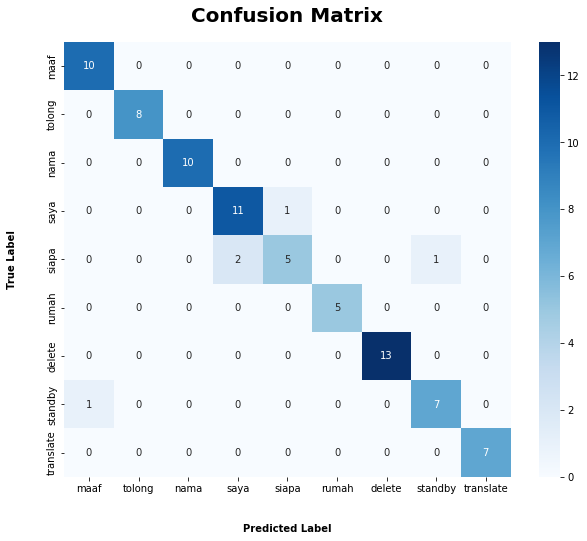
\includegraphics[scale=0.55]{gambar/bab4-uji-model-second-cf.png}

  \caption{\emph{Confusion} model kedua}
  \label{fig:model2-cf}
\end{figure}

\begin{longtable}{|c|c|c|c|c|}
  \caption{Matrix Evaluasi Model 2}
  \label{tb:model2stat}                                   \\
  \hline
  \rowcolor[HTML]{C0C0C0}
  \textbf{Kosakata} & \textbf{\emph{Accuracy}} & \textbf{\emph{Precision}} & \textbf{\emph{Recall}} & \textbf{\emph{F1-Score}} \\
  \hline
  Maaf              & 1.00                        & 0.91                        & 1.00                   & 0.95                \\
  Tolong            & 1.00                        & 1.00                        & 1.00                   & 1.00                \\
  Nama              & 1.00                        & 1.00                        & 1.00                   & 1.00                \\
  Saya              & 0.91                        & 0.85                        & 0.92                   & 0.88                \\
  Siapa             & 0.62                        & 0.93                        & 0.62                   & 0.71                \\
  Rumah             & 1.00                        & 1.00                        & 1.00                   & 1.00                \\
  Delete            & 1.00                        & 1.00                        & 1.00                   & 1.00                \\
  Standby           & 0.87                        & 0.88                        & 0.88                   & 0.88                \\
  Translate         & 1.00                        & 1.00                        & 1.00                   & 1.00                \\
  \hline
\end{longtable}

\subsection{Model Ketiga}
\label{sec:analisismodel3}

\begin{figure}[H]
  \centering

  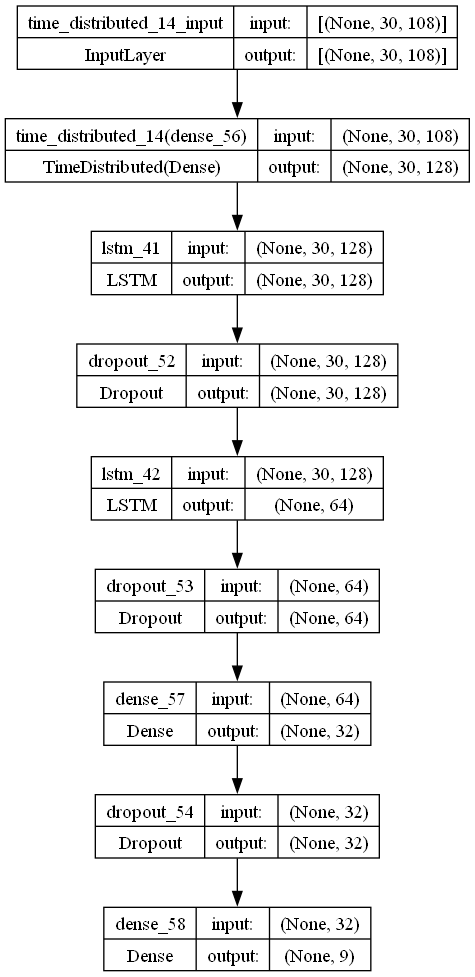
\includegraphics[scale=0.6]{gambar/bab4-uji-model-best-model.png}

  \caption{Struktur model ketiga}
  \label{fig:model3-struktur}
\end{figure}

Model ketiga merupakan gabungan dari struktur antara model 1 dan model 2. Model ini diawali dengan layer pertama berupa \emph{layer} \textit{TimeDistributed} yang di dalamnya terdapat \emph{layer} \textit{Dense} dengan fungsi aktivasi '\textit{tanh}' dan unit aktivasi bernilai 128. Selanjutnya diikuti dengan 2 buah \emph{layer} LSTM. \emph{Layer} LSTM pertama menggunakan fungsi aktivasi \emph{tanh} dengan unit aktivasi bernilai 128 dan \emph{Layer} LSTM kedua menggunakan fungsi aktivasi \emph{tanh} dengan unit aktivasi bernilai 64. Kedua \emph{layer} LSTM ini diikuti dengan \emph{layer} Dropout bernilai 0.5 untuk mencegah nilai \emph{weight} yang terlalu tinggi. Dilanjutkan dengan \emph{layer} Dense dengan fungsi aktivasi \emph{relu} dan unit aktivasi bernilai 32. Struktur lengkap dari model ini dapat dilihat pada gambar \ref{fig:model3-struktur}

\begin{figure}[H]
  \centering

  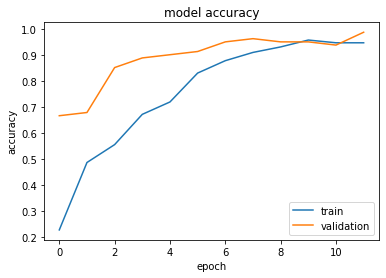
\includegraphics[scale=0.75]{gambar/bab4-uji-model-best-acc.png}

  \caption{Hasil \emph{accuracy} model ketiga}
  \label{fig:model3-train-acc}
\end{figure}

\begin{figure}[H]
  \centering

  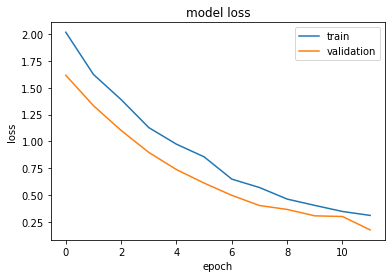
\includegraphics[scale=0.75]{gambar/bab4-uji-model-best-loss.png}

  \caption{Hasil \emph{loss} model ketiga}
  \label{fig:model3-train-loss}
\end{figure}

Berdasarkan dari \emph{training} yang telah dilakukan didapatkan bahwa model menghasilkan akurasi \emph{training} bernilai 0.94 dan akurasi validasi bernilai 1.00. Data ini menunjukkan bahwa model memiliki akurasi yang sangat baik. Untuk nilai \emph{loss training} bernilai 0.3 dan \emph{loss} validasi bernilai 0.16 yang rendah jika dibandingkan dengan nilai \emph{loss training}. Data ini menunjukkan bahwa model memiliki \emph{error} prediksi yang kecil. Hasil dari \emph{training} model ini menunjukkan bahwa model telah dapat mempelajari dataset dengan baik. Ketika dilakukan pengujian dengan menggunakan data validasi, dapat dilihat bahwa model memiliki akurasi yang lebih tinggi dan tingkat \emph{loss} yang lebih rendah dibandingkan dengan pengujian yang menggunakan data \emph{training} itu sendiri. Grafik akurasi dan \emph{loss} dapat dilihat pada gambar \ref{fig:model3-train-acc} dan gambar \ref{fig:model3-train-loss}.


Kemudian berdasarkan model yang telah dihasilkan, dilakukan pengujian dengan dataset \emph{testing} yang menghasilkan \emph{confusion matrix}. Dapat dilihat pada gambar \ref{fig:model3-cf}, untuk kosakata "maaf", "tolong", "nama", "saya",  menghasilkan prediksi yang tepat untuk keseluruhan dataset \emph{testing} yang diujikan. Namun, pada kosakata "siapa" menghasilkan beberapa prediksi yang tidak sesuai dengan dataset \emph{testing}. Kosakata "siapa" menghasilkan 7 prediksi tepat dan 1 prediksi yang kurang tepat (dataset \emph{testing} bernilai "saya"). Dapat dilihat bahwa terdapat peningkatan performa dari model ketiga dibandingkan dengan model pertama dan kedua. Peningkatan ini disebabkan karena perubahan struktur dari model dengan penggunaan \emph{layer Time Distributed} yang didalamnya diisi dengan \emph{layer} Dense di lapisan awal model. Kemudian dilanjutkan dengan 2 buah \emph{layer} LSTM yang menggunakan fungsi aktivasi \emph{tanh} Adapun berdasarkan \emph{confusion matrix} ini didapat matrix evaluasi berupa \emph{accuracy}, \emph{precision}, \emph{recall}, dan \emph{F1-score} yang dapat dilihat pada tabel \ref{tb:model3stat}. Rata - rata nilai \emph{accuracy} sebesar 0.99, rata - rata nilai \emph{precision} sebesar 0.99 rata - rata nilai \emph{recall} sebesar 0.98, dan rata - rata nilai \emph{F1-score} sebesar 0.99. Dapat dilihat berdasarkan matrix evaluasi ini, terdapat peningkatan performa pada model ketiga jika dibandingkan dengan model pertama dan kedua.

\begin{figure}[H]
  \centering

  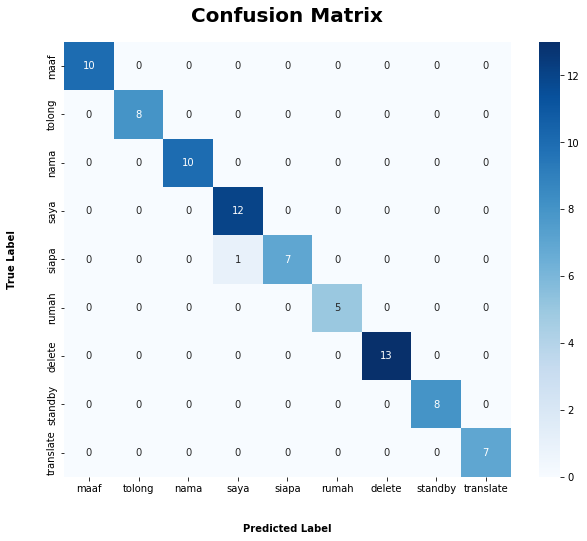
\includegraphics[scale=0.6]{gambar/bab4-uji-model-best-cf.png}

  \caption{\emph{Confusion} model ketiga}
  \label{fig:model3-cf}
\end{figure}

\begin{longtable}{|c|c|c|c|c|c|}
  \caption{Matrix Evaluasi Model 3}
  \label{tb:model3stat}                                   \\
  \hline
  \rowcolor[HTML]{C0C0C0}
  \textbf{Kosakata} & \textbf{\emph{Accuracy}} & \textbf{\emph{Precision}} & \textbf{\emph{Recall}} & \textbf{\emph{F1-Score}} \\
  \hline
  Maaf              & 1.00                       & 1.00                        & 1.00                   & 1.00                \\
  Tolong            & 1.00                       & 1.00                        & 1.00                   & 1.00                \\
  Nama              & 1.00                       & 1.00                        & 1.00                   & 1.00                \\
  Saya              & 1.00                       & 0.92                        & 1.00                   & 0.96                \\
  Siapa             & 0.87                       & 1.00                        & 0.82                   & 0.93                \\
  Rumah             & 1.00                       & 1.00                        & 1.00                   & 1.00                \\
  Delete            & 1.00                       & 1.00                        & 1.00                   & 1.00                \\
  Standby           & 1.00                       & 1.00                        & 1.00                   & 1.00                \\
  Translate         & 1.00                       & 1.00                        & 1.00                   & 1.00                \\
  \hline
\end{longtable}

\subsection{Rangkuman Pengujian Bentuk Model}
\label{sec:analisismodelseluruh}

\begin{longtable}{|c|c|c|c|c|}
  \caption{Rangkuman Pengujian Bentuk Model}
  \label{tb:evaluasiModel}                                   \\
  \hline
  \rowcolor[HTML]{C0C0C0}
  \textbf{Model} & \emph{\textbf{Avg. Accuracy}} & \emph{\textbf{Avg. Precision}} & \emph{\textbf{Avg. Recall}} & \emph{\textbf{Avg. F1-Score}} \\
  \hline
  Model 1 & 0.85 & 0.85 & 0.85 & 0.83 \\
  Model 2 & 0.93 & 0.95 & 0.94 & 0.94 \\
  Model 3 & 0.99 & 0.99 & 0.98 & 0.99 \\
  \hline
\end{longtable}

Secara keseluruhan, berdasarkan tabel \ref{tb:evaluasiModel} bahwa seiring denagn peningkatan kompleksitas dari suatu model selaras dengan peningkatan performa dari model itu sendiri. Hal ini dapat ditunjukkan dengan peningkatan akurasi dari model 1, yaitu 0.85 atau 85\% menjadi pada model 3, yaitu 0.99 atau 99\%. Nilai \emph{average precision}, {average recall},dan \emph{average F1-Score} juga meningkat seiring dengan peningkatan stuktur dari model. Penggunaan \emph{layer TimeDistributed} dan diikuti 2 \emph{layer} LSTM menghasilkan model dengan performa terbaik.

Adapun pada setiap \emph{class} yang ada menunjukkan bahwa performa kosakata 'siapa' menghasilkan hasil klasifikasi yang kurang baik. Hal ini dapat dipengaruhi oleh adanya kempiripan antara kosakata ini dengan berbagai kosakata lainnya. Pergerakan isyarat kosakata 'siapa' berfokus pada gerakan tangan yang mengarah ke depan subjek. Gerakan ini mengutamakan kedinamisan antara koordinat y yang berubah seiring dengan pergerakan tangan. Kosakata 'saya' juga memiliki fokus gerakan isyarat yang secara garis besar sama, yaitu gerakan tangan yang mengarah ke depan subjek. Hal ini menyebabkan model kesulitan dalam memberikan klasifikasi yang tepat dan cenderung \emph{overfitting} pada kosakata 'saya'. Apabila dilihat dari peresebaran kooridnat yang ada, didapat bahwa koordinat kosakata 'saya' dan 'siapa' memiliki lingkup persebaran yang hampir sama yang dapat dilihat pada gambar \ref{fig:isyarat-coor-saya} dan gambar \ref{fig:isyarat-coor-siapa}, dimana terdapat 3 'daerah' persebaran yang hampir sama. 



\begin{figure}[H]
  \centering

  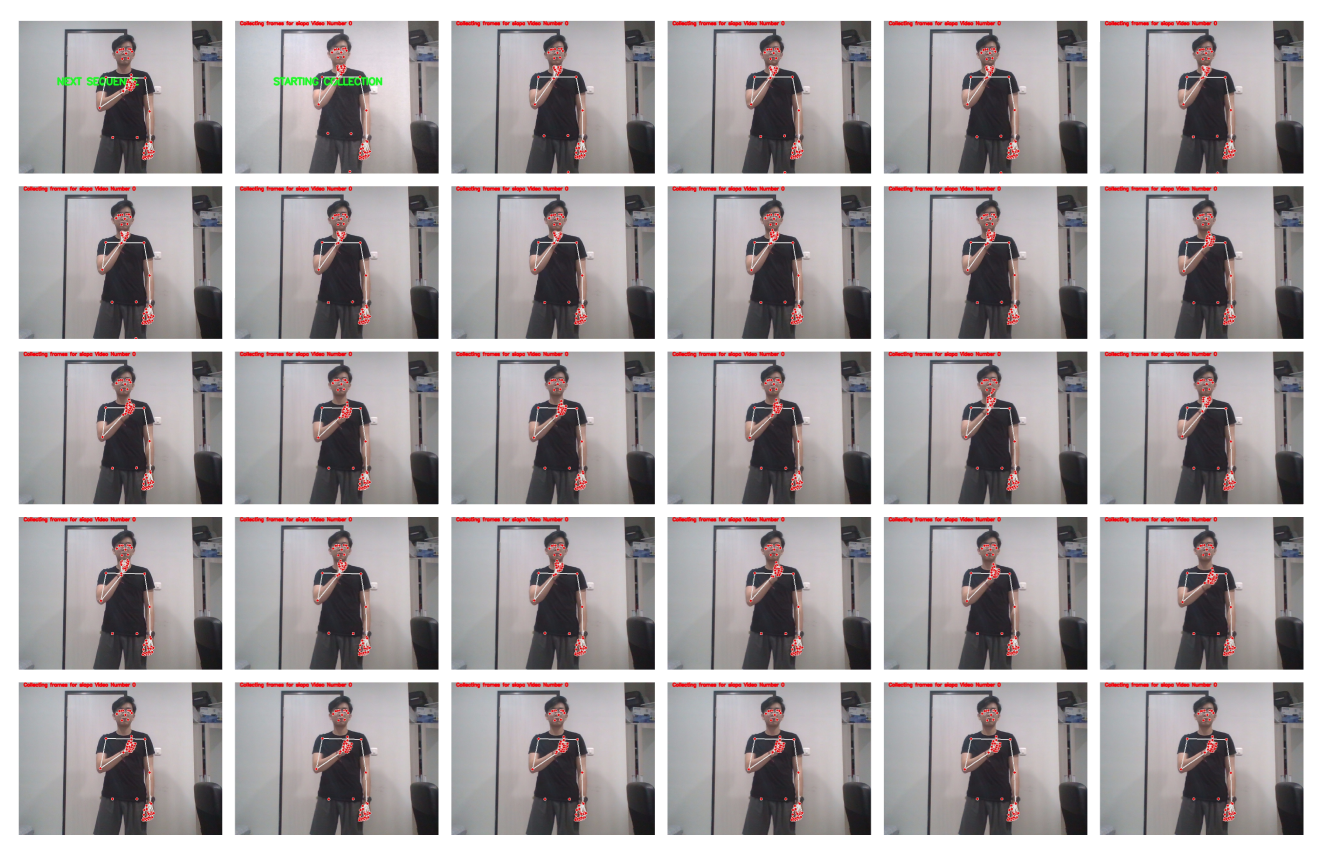
\includegraphics[scale=0.45]{gambar/isyarat-siapa.png}

  \caption{Isyarat kosakata 'siapa'}
  \label{fig:isyarat-siapa}
\end{figure}

\begin{figure}[H]
  \centering

  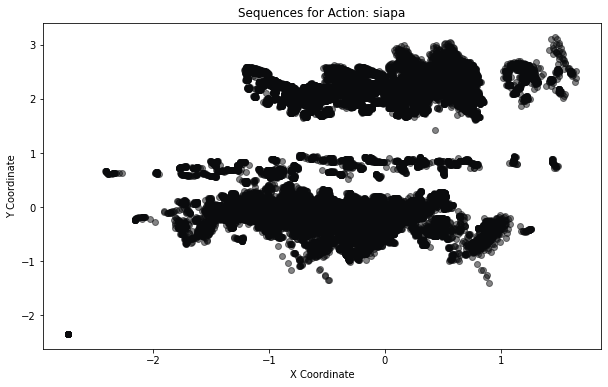
\includegraphics[scale=0.7]{gambar/coor-siapa.png}

  \caption{Persebaran koordinat kosakata 'siapa'}
  \label{fig:isyarat-coor-siapa}
\end{figure}

\begin{figure}[H]
  \centering

  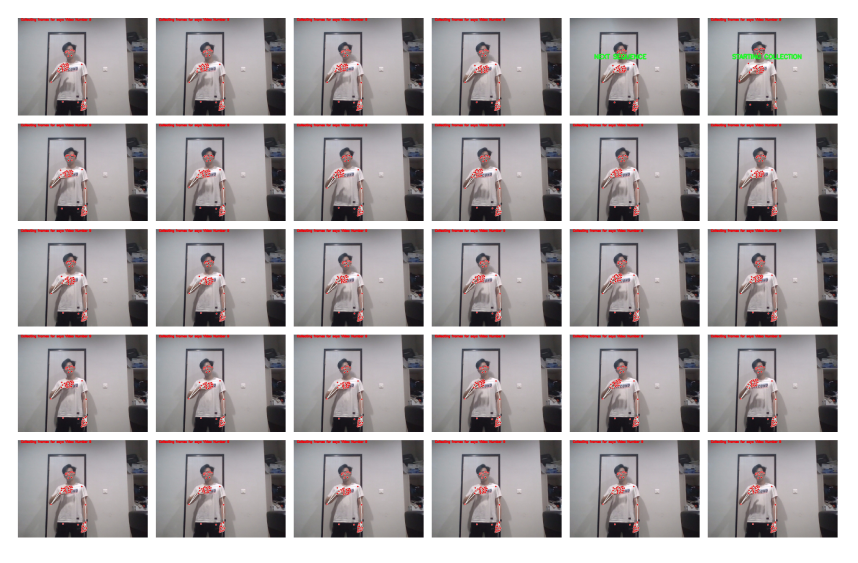
\includegraphics[scale=0.7]{gambar/isyarat-saya.png}

  \caption{Isyarat kosakata 'saya'}
  \label{fig:isyarat-saya}
\end{figure}

\begin{figure}[H]
  \centering

  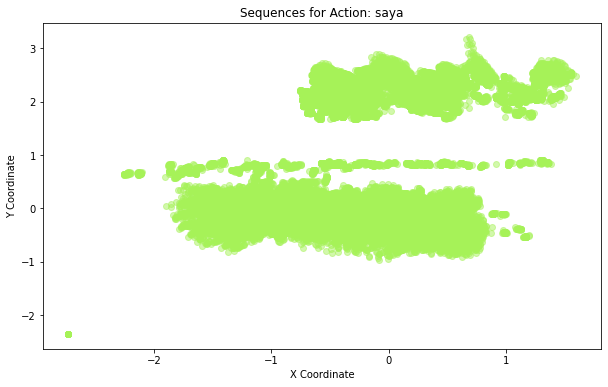
\includegraphics[scale=0.7]{gambar/coor-saya.png}

  \caption{Persebaran koordinat 'saya'}
  \label{fig:isyarat-coor-saya}
\end{figure}

\newpage
\section{Pengujian Kondisi Cahaya}
\label{sec:analisiscahaya}

\begin{longtable}{|c|c|}
  \caption{Variasi Kondisi Cahaya}
  \label{tb:kondisicahaya}                                   \\
  \hline
  \rowcolor[HTML]{C0C0C0}
  \textbf{Intensitas Cahaya} & \textbf{Gambar Kondisi}  \\
  \hline
  35 lux            &  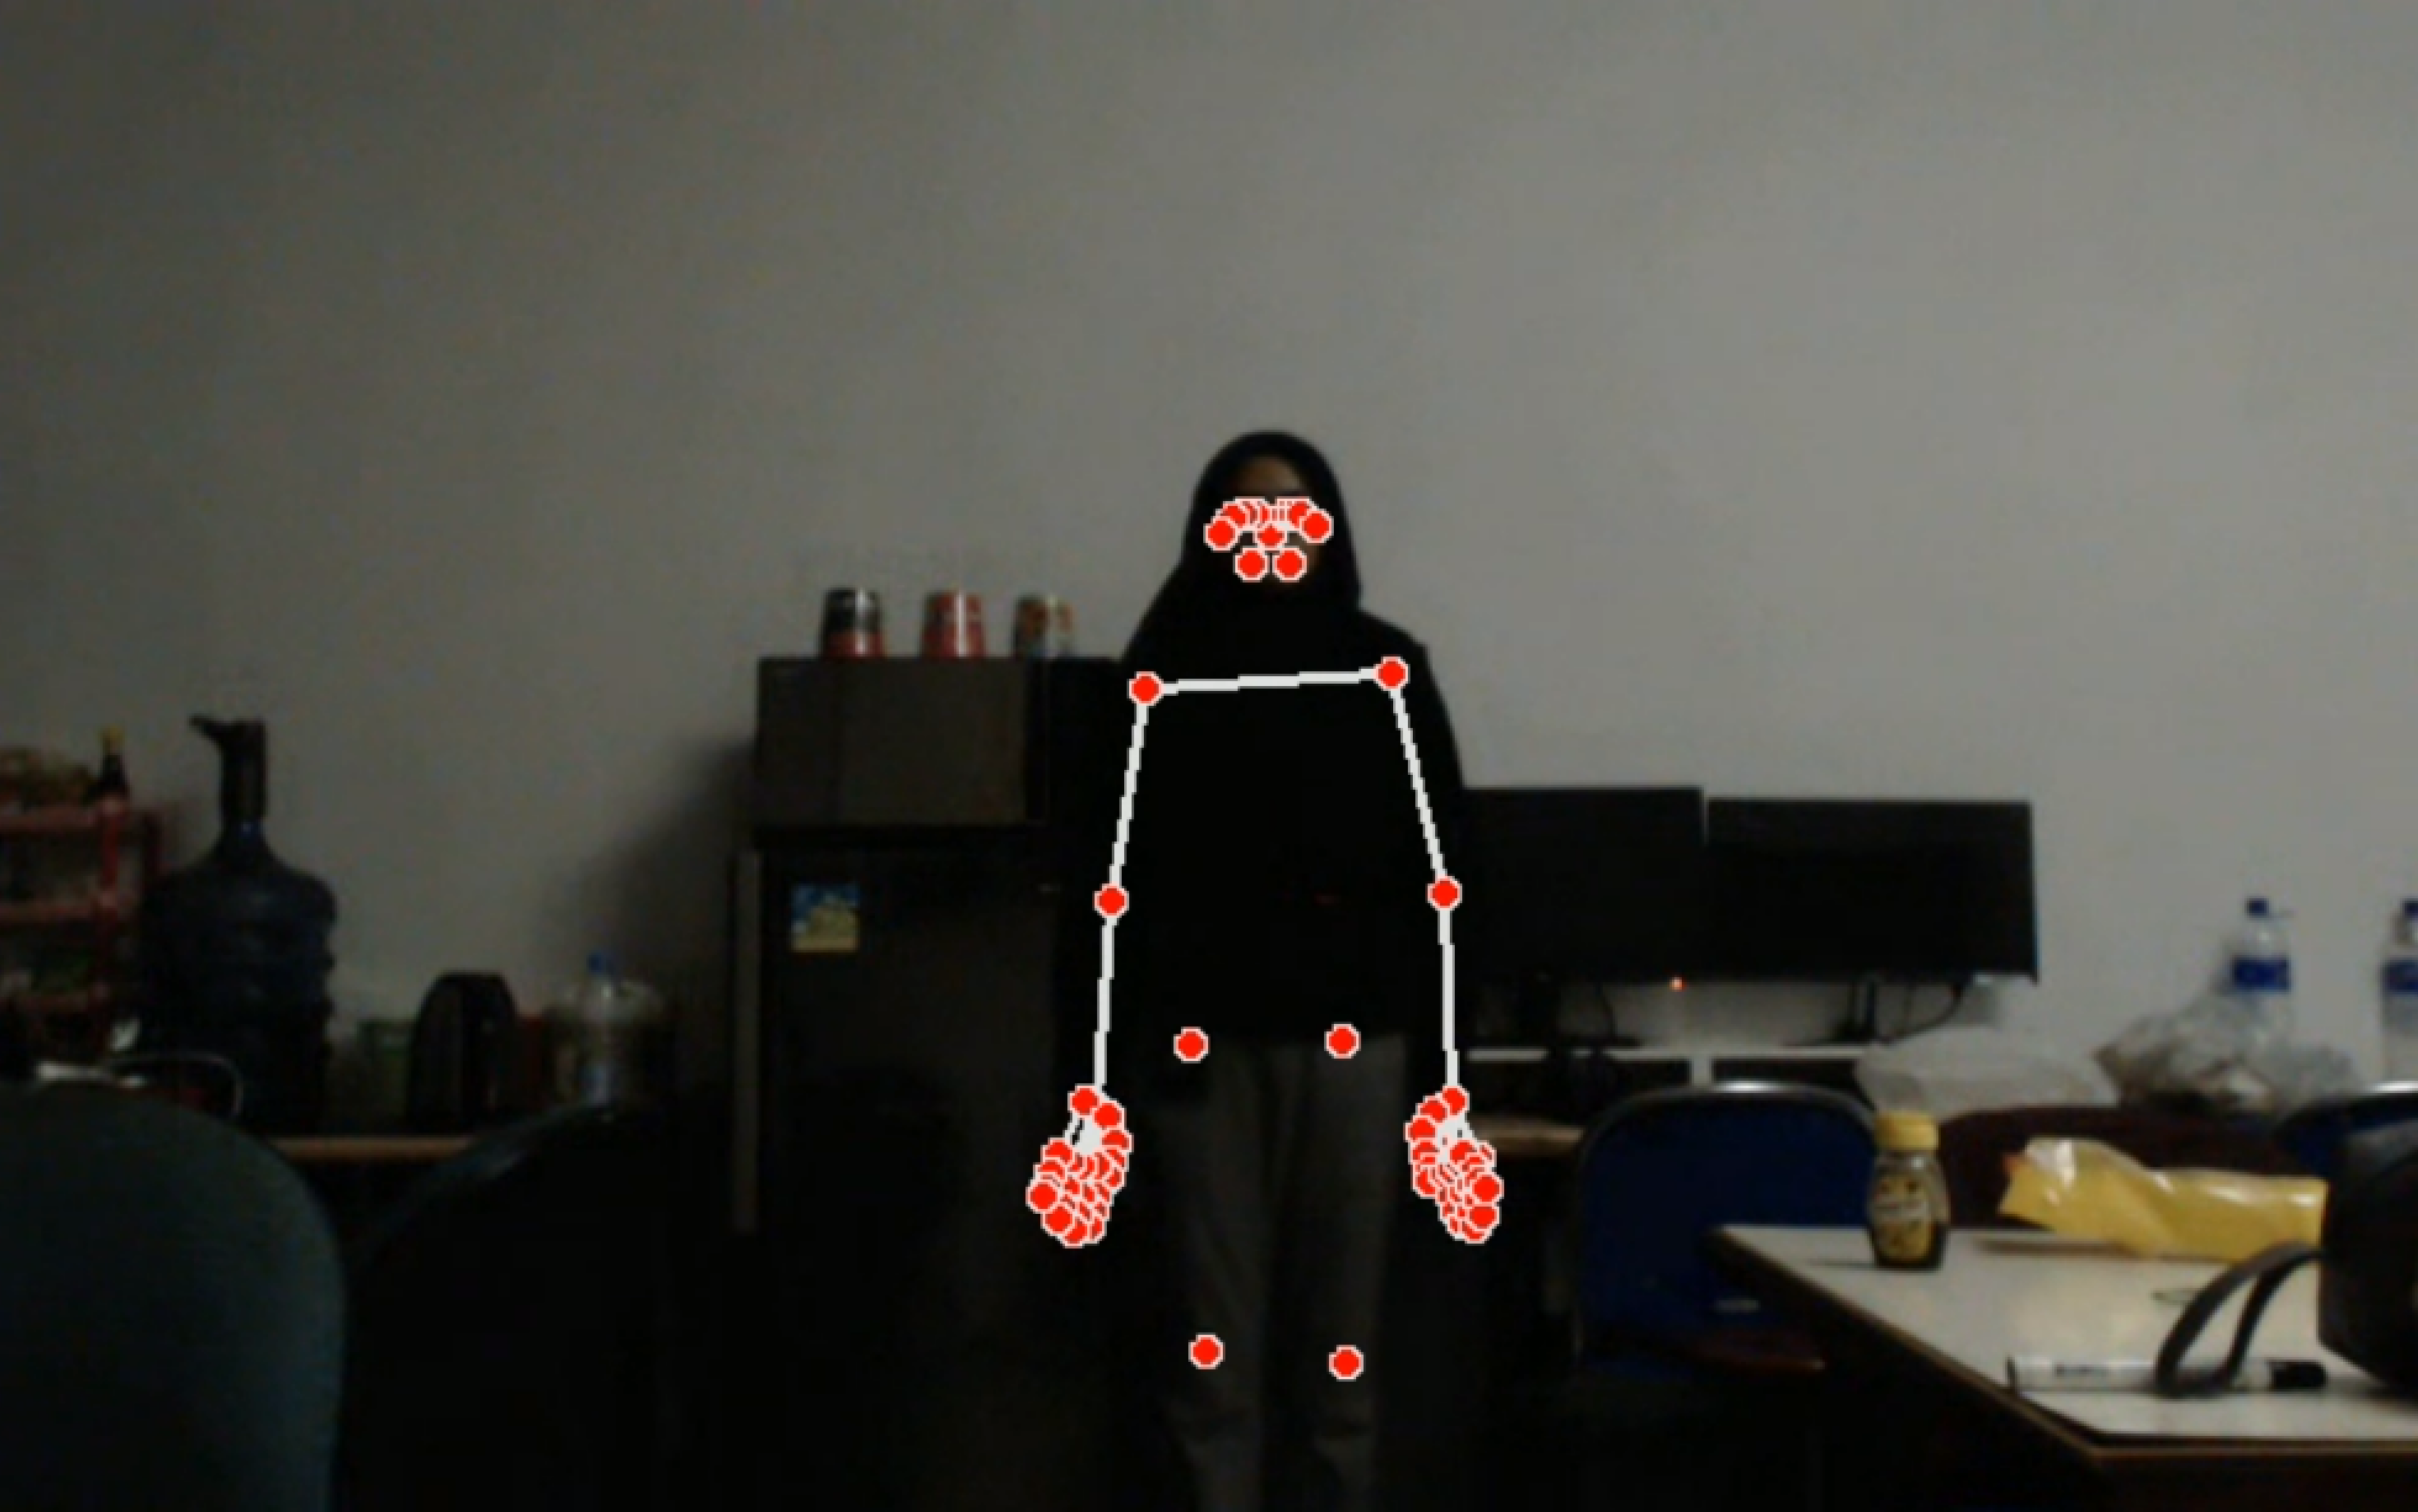
\includegraphics[scale=0.3]{gambar/bab4-gelap.png}                \\
  \hline
  80 lux            & 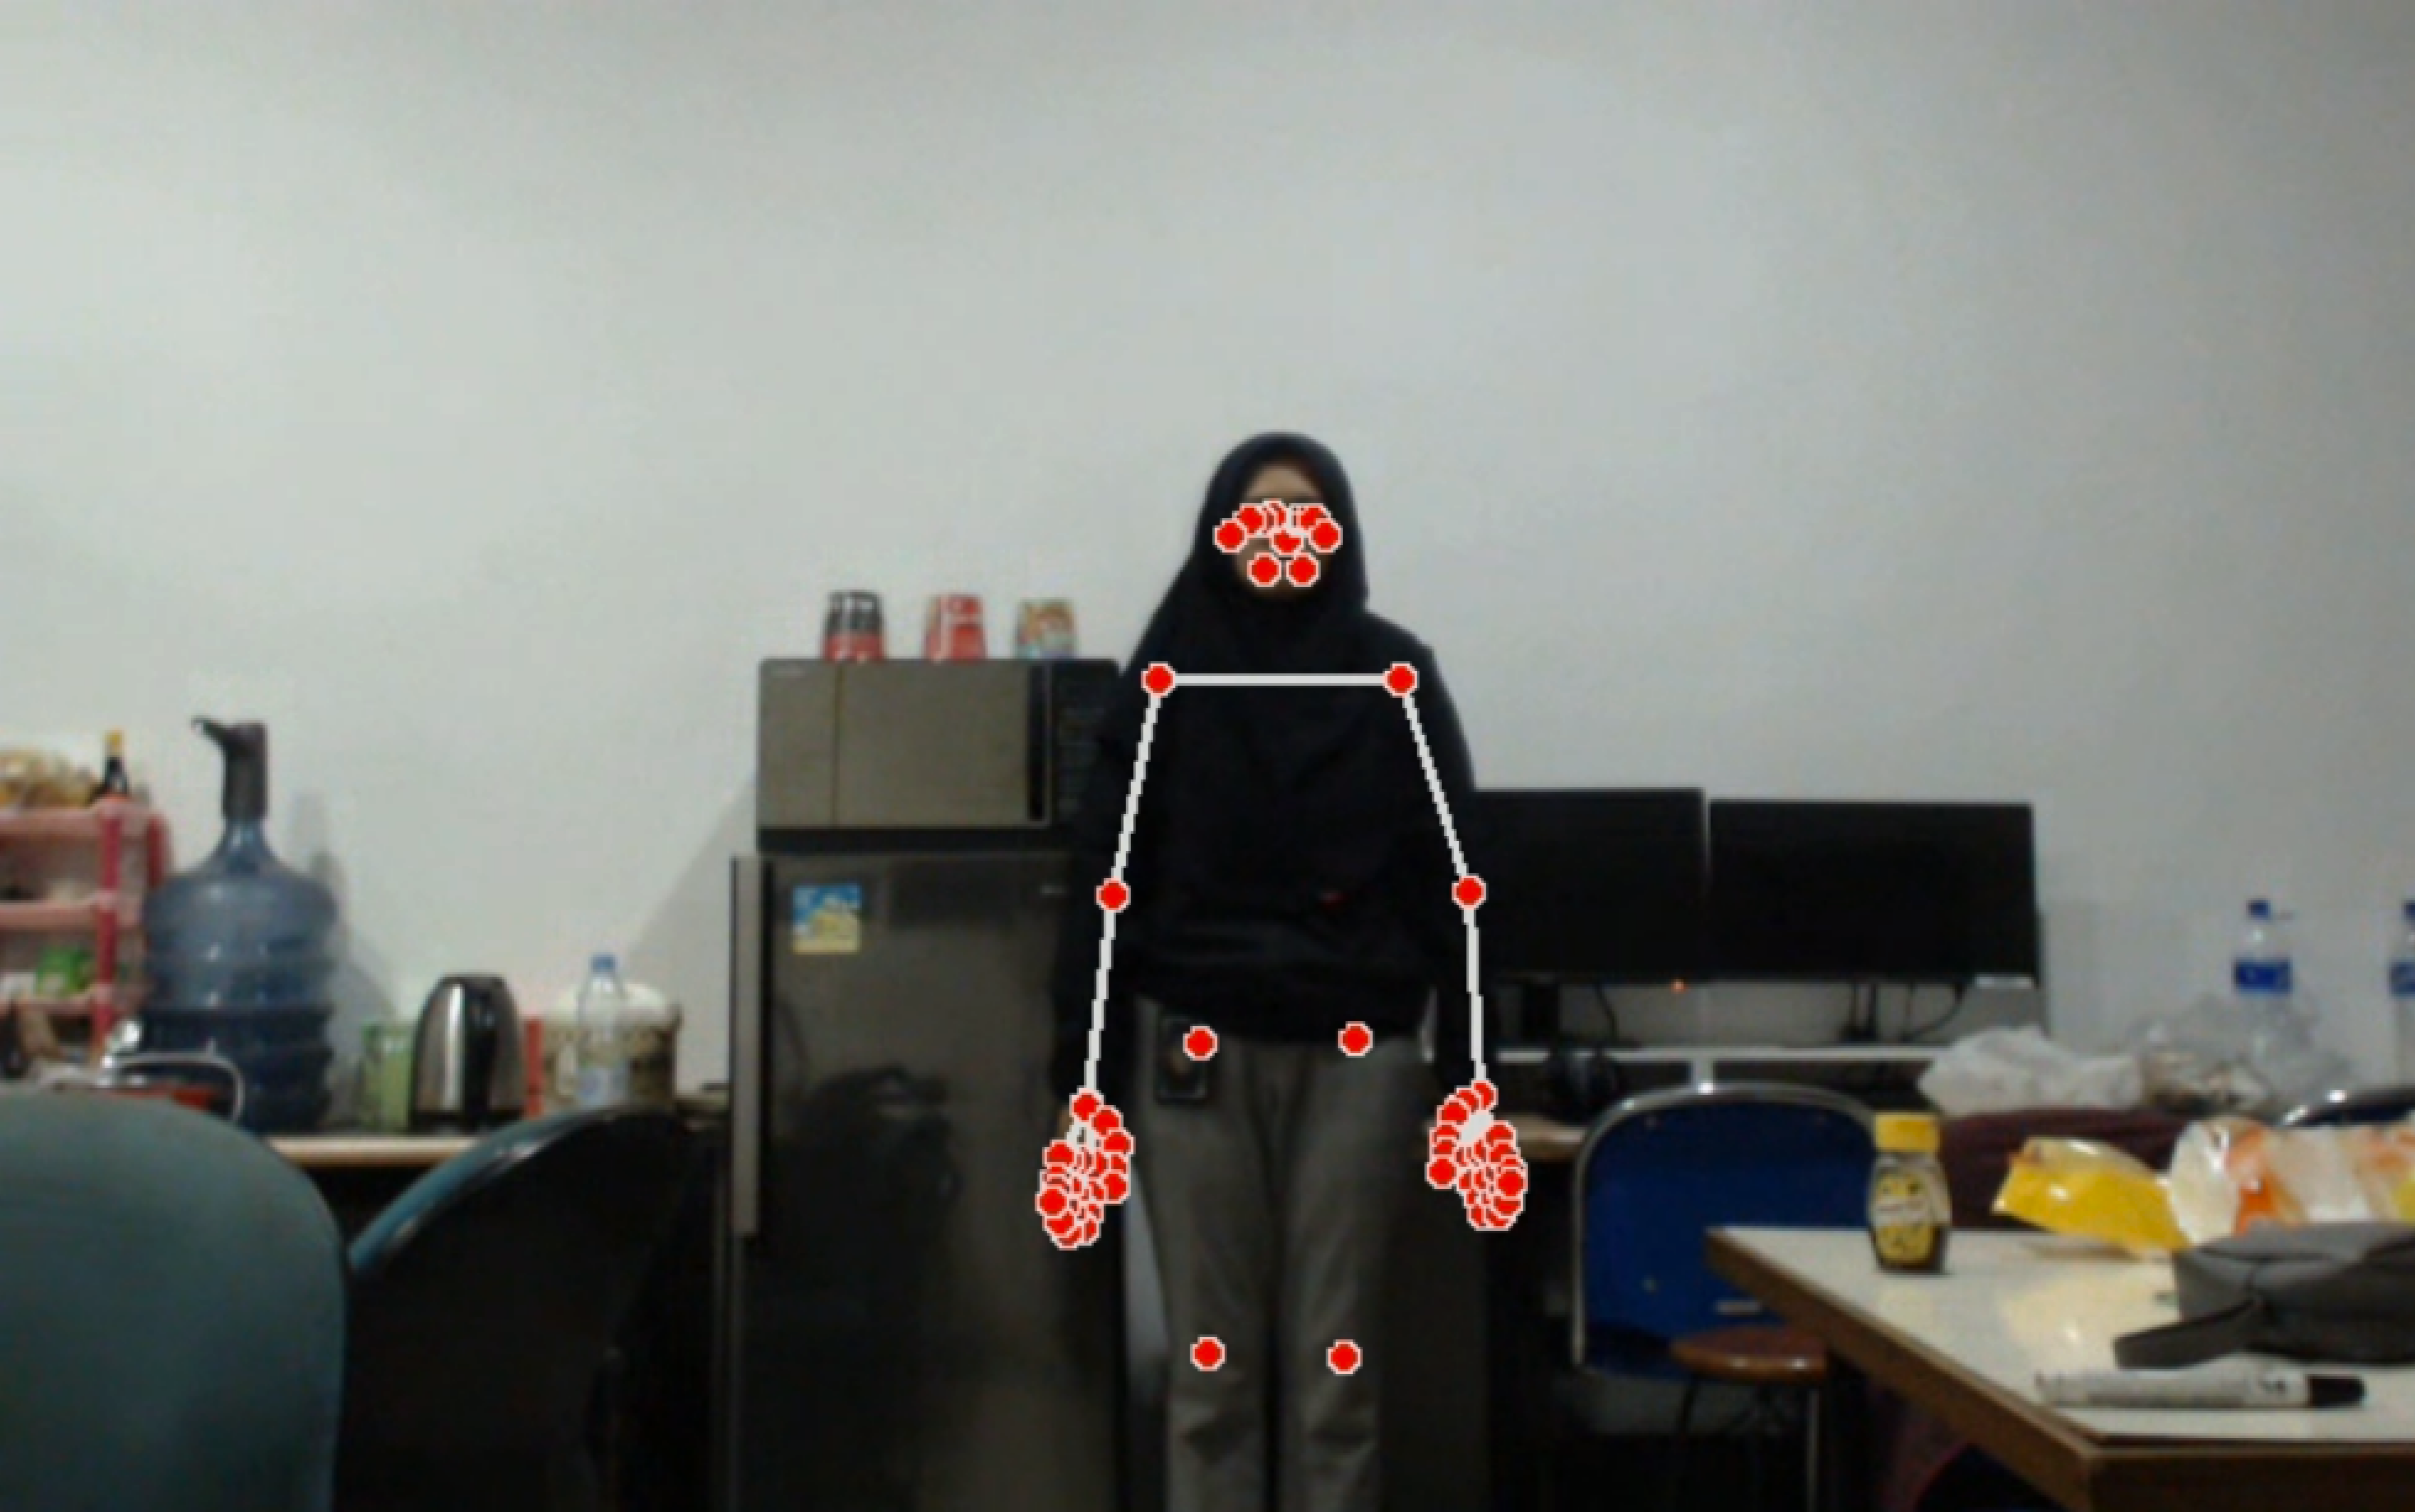
\includegraphics[scale=0.3]{gambar/bab4-remang.png}                 \\
  \hline
  125 lux            & 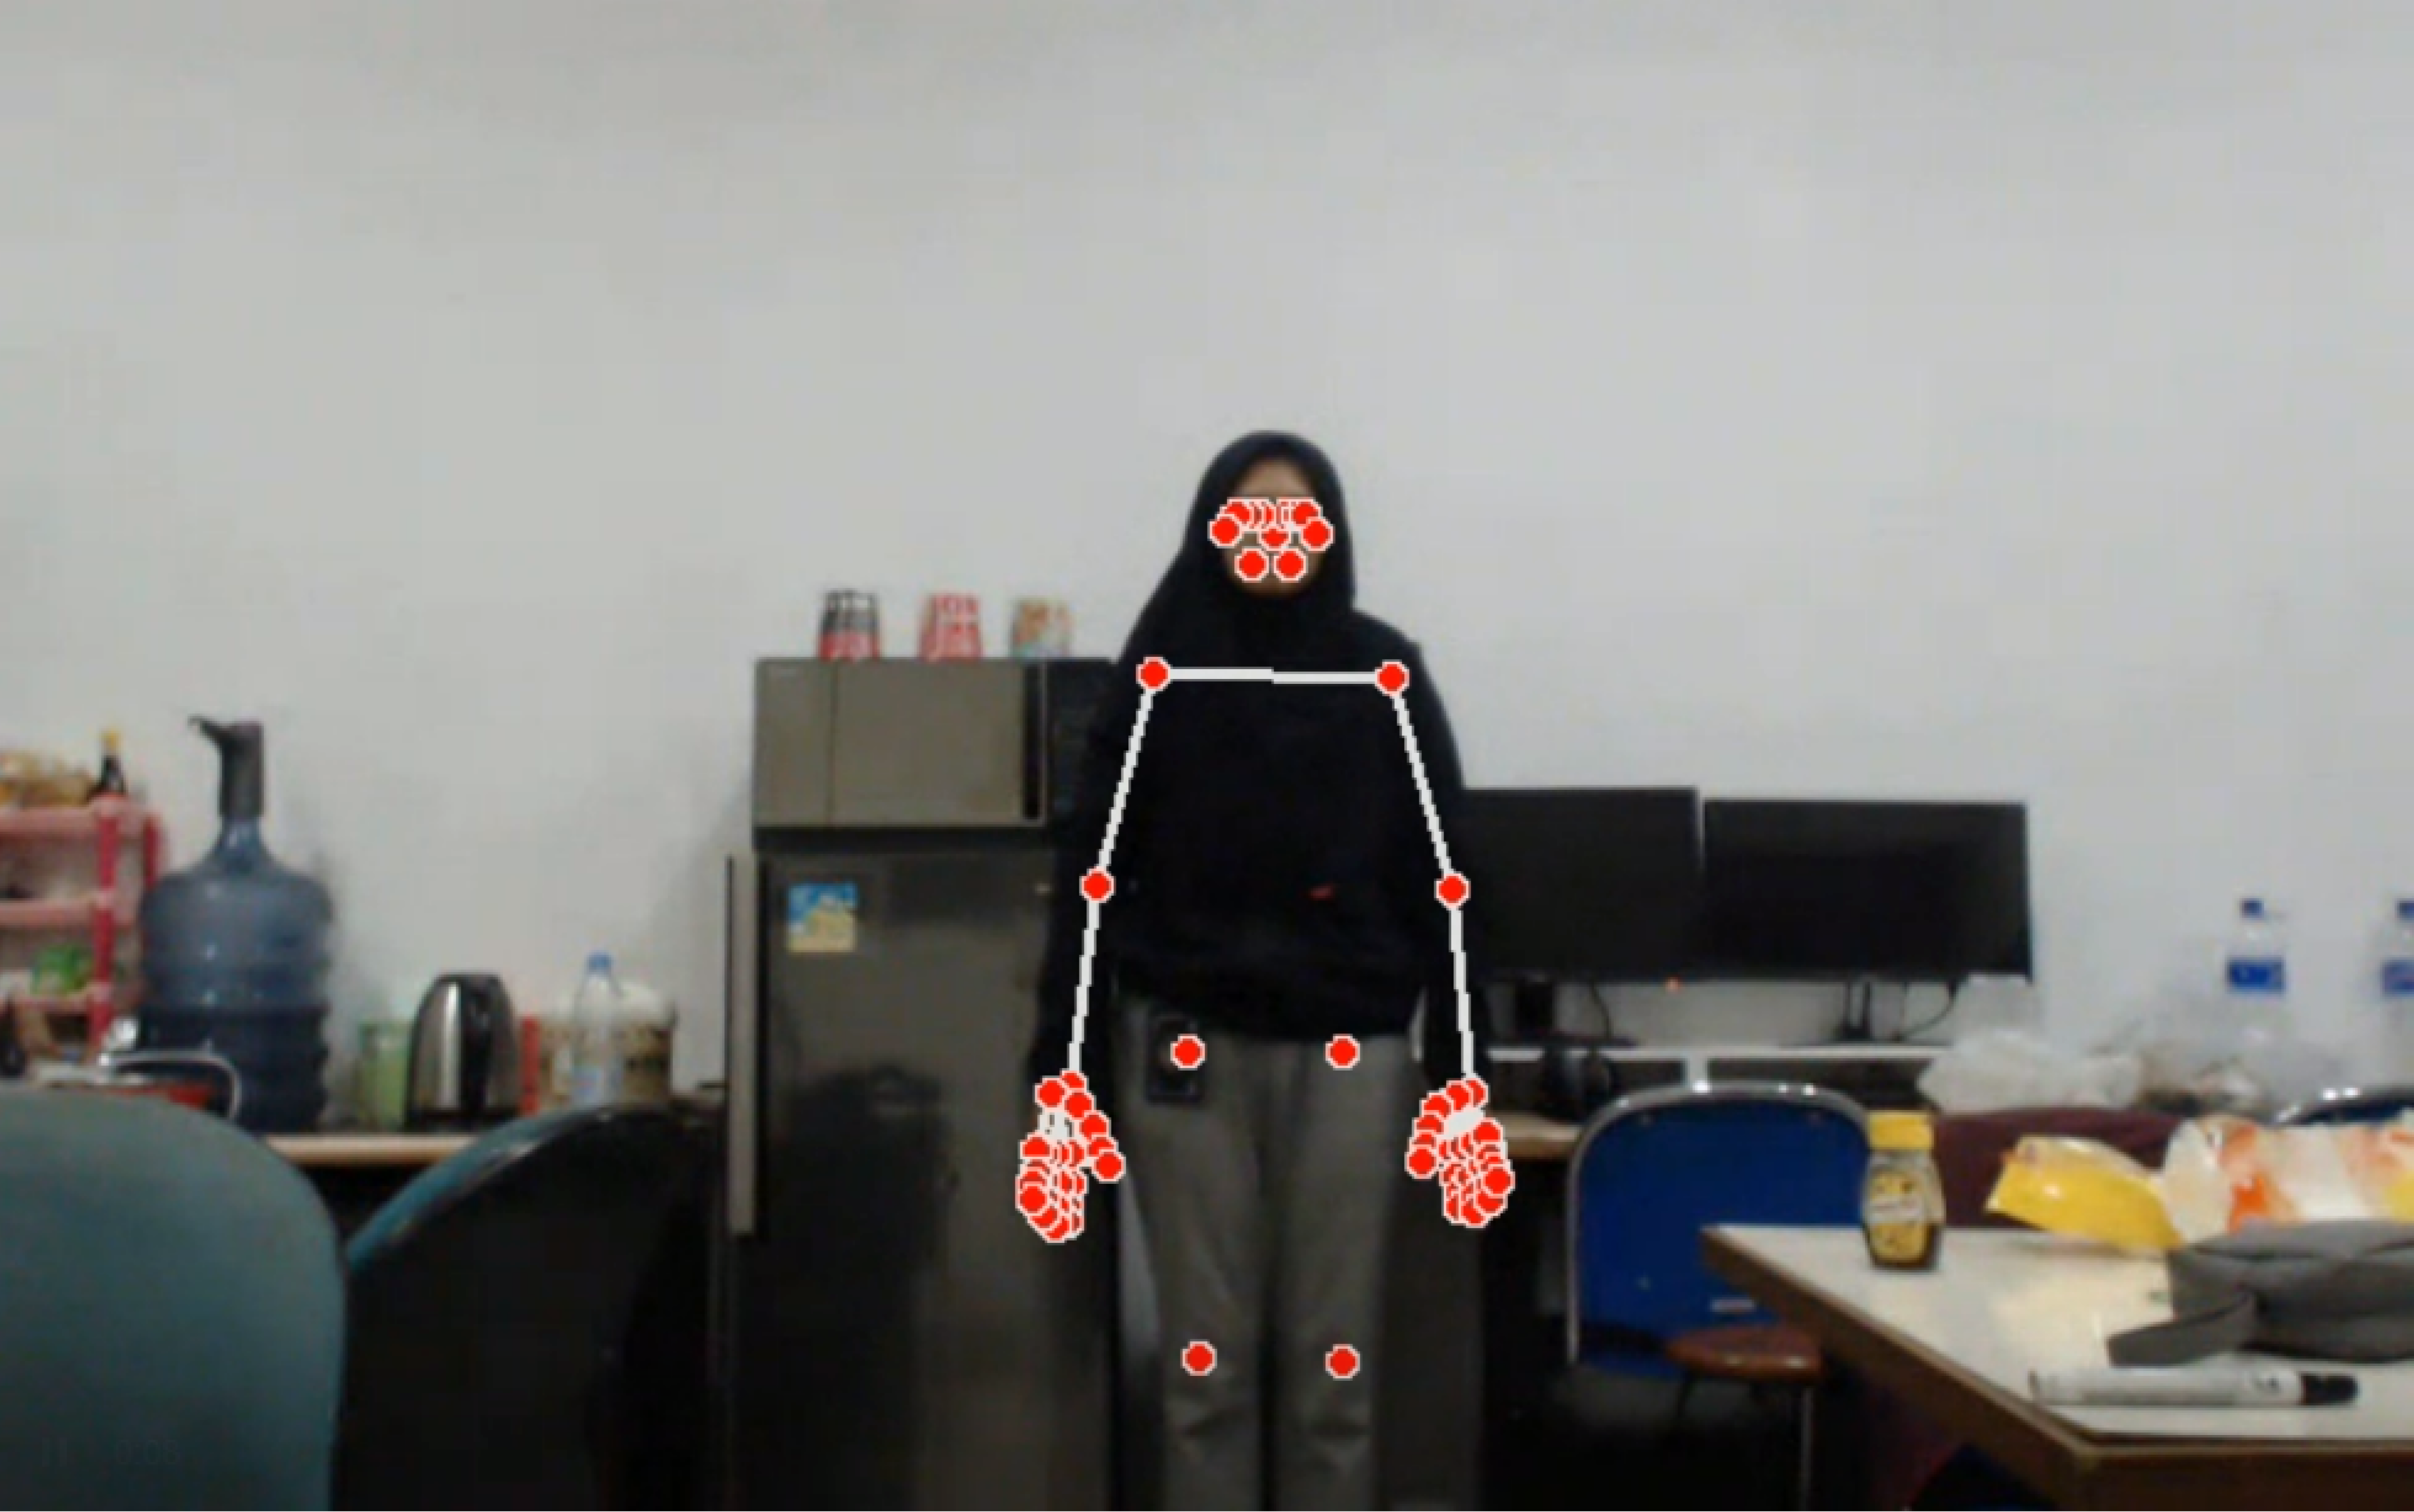
\includegraphics[scale=0.3]{gambar/bab4-terang.png}                 \\
  \hline
\end{longtable}

Pada pengujian kondisi cahaya ini dilakukan untuk memahami bagaimana performa model dalam kondisi intensitas cahaya  yang berbeda - beda. Adapun intensitas cahaya yang akan digunakan pada pengujian ini adalah 35 lux (kondisi ruangan gelap), 80 lux (kondisi ruangan remang - remang), dan 125 lux (kondisi ruangan terang). Variasi intensitas cahaya ini dipilih karena merupakan intensitas cahaya yang umum ditemukan pada ruangan tertutup. Kondisi ruangan dengan intensitas cahaya masing - masing dapat dilihat pada tabel \ref{tb:kondisicahaya}. Pengambilan nilai intensitas cahaya ini dilakukan dengan menggunakan \emph{lux meter} yang telah dikalibrasi untuk memastikan ketelitian hasil pengukuran.

Model penerjemah bahasa Indonesia (BISINDO) yang akan digunakan pada pengujian ini adalah model pada bagian \ref{sec:analisismodel3} karena merupakan model yang menghasilkan klasifikasi yang terbaik jika dibandingkan dengan model lainnya. Untuk setiap intensitas cahaya akan dilakukan pengujian sebanyak tiga kali dengan jarak terhadap kamera sebesar 300 cm. Pada setiap pengujian akan dicari hasil klasifikasi model, waktu yang dibutuhkan model untuk menghasilkan klasifikasi bahasa isyarat berdasarkan data koordinat yang diberikan(\emph{processing time}), waktu total yang dibutuhkan dalam menghasilkan klasifikasi bahasa isyarat (\emph{complete time}), dan rata - rata FPS (\emph{frame per second}) yang didapatkan ketika proses klasifikasi dilakukan pada website.  

\subsection{Pengujian Model di Kondisi Cahaya 35 lux}
\label{sec:analisiscahaya1}

\begin{longtable}{|c|c|c|c|c|}
  \caption{Pengujian Pertama Model di Kondisi Cahaya 35 lux}
  \label{tb:prediksigelap1}                                   \\
  \hline
  \rowcolor[HTML]{C0C0C0}
  \textbf{Kosakata} & \textbf{Klasifikasi Model} & \textbf{\emph{Processing Time}} & \textbf{\emph{Complete Time}} & \textbf{\emph{FPS}}\\
  \hline
  Maaf              & Maaf                          & 0.09209 detik                           & 2.87358 detik                                  & 10.43992871\\
  Tolong            & Tolong                        & 0.09198 detik                           & 2.90961 detik                                  & 10.31065923\\
  Nama              & Nama                          & 0.08932 detik                           & 3.32747 detik                                  & 9.015859368\\
  Saya              & Saya                          & 0.09867 detik                           & 2.88227 detik                                  & 10.40845123\\
  Siapa             & Siapa                         & 0.08973 detik                           & 2.85298 detik                                  & 10.51530802\\
  Rumah             & \textcolor{red}{Delete}       & 0.09612 detik                           & 2.86434 detik                                  & 10.47361061\\
  Delete            & Delete                        & 0.09255 detik                           & 2.82485 detik                                  & 10.62005054\\
  Standby           & Standby                       & 0.09247 detik                           & 2.87624 detik                                  & 10.43027096\\
  Translate         & Translate                     & 0.09525 detik                           & 2.92625 detik                                  & 10.25203914\\
  \hline
\end{longtable}

\begin{longtable}{|c|c|c|c|c|}
  \caption{Pengujian Kedua Model di Kondisi Cahaya 35 lux}
  \label{tb:prediksigelap2}                                   \\
  \hline
  \rowcolor[HTML]{C0C0C0}
  \textbf{Kosakata} & \textbf{Klasifikasi Model} & \textbf{\emph{Processing Time}} & \textbf{\emph{Complete Time}} & \textbf{\emph{FPS}}\\
  \hline
  Maaf              & Maaf                            & 0.10043 detik                           & 3.32854 detik                                   & 9.012933934\\
  Tolong            & Tolong                          & 0.09723 detik                           & 3.31908 detik                                   & 9.038649602\\
  Nama              & \textcolor{red}{Standby}        & 0.08973 detik                           & 2.91430 detik                                   & 10.29405889\\
  Saya              & Saya                            & 0.10072 detik                           & 2.78958 detik                                   & 10.75429474\\
  Siapa             & Siapa                           & 0.08973 detik                           & 3.40174 detik                                   & 8.818992471\\
  Rumah             & Rumah                           & 0.10046 detik                           & 2.94283 detik                                   & 10.19425527\\
  Delete            & Delete                          & 0.09255 detik                           & 2.91633 detik                                   & 10.28691395\\
  Standby           & Standby                         & 0.09182 detik                           & 2.82681 detik                                   & 10.61268775\\
  Translate         & Translate                       & 0.08920 detik                           & 3.39125 detik                                   & 8.846297753\\
  \hline
\end{longtable}


\newpage
\begin{longtable}{|c|c|c|c|c|}
  \caption{Pengujian Ketiga Model di Kondisi Cahaya 35 lux}
  \label{tb:prediksigelap3}                                   \\
  \hline
  \rowcolor[HTML]{C0C0C0}
  \textbf{Kosakata} & \textbf{Klasifikasi Model} & \textbf{\emph{Processing Time}} & \textbf{\emph{Complete Time}} & \textbf{\emph{FPS}}\\
  \hline
  Maaf              & Maaf                          & 0.09209 detik                           & 2.91590 detik                                  & 10.28842795\\
  Tolong            & Tolong                        & 0.09723 detik                           & 3.00149 detik                                  & 9.995029061\\
  Nama              & Nama                          & 0.09725 detik                           & 2.82353 detik                                  & 10.62500063\\
  Saya              & Saya                          & 0.08916 detik                           & 2.96069 detik                                  & 10.13275997\\
  Siapa             & Siapa                         & 0.08973 detik                           & 2.84085 detik                                  & 10.56023606\\
  Rumah             & \textcolor{red}{Delete}       & 0.10066 detik                           & 3.36672 detik                                  & 8.910741828\\
  Delete            & Delete                        & 0.09255 detik                           & 3.43082 detik                                  & 8.744254311\\
  Standby           & Standby                       & 0.09867 detik                           & 3.34507 detik                                  & 8.968416101\\
  Translate         & Translate                     & 0.08920 detik                           & 2.83052 detik                                  & 10.5987426\\
  \hline
\end{longtable}


Berdasarkan tiga pengujian yang telah dilakukan, didapatkan bahwa hampir keseluruhan klasifikasi model yang sesuai dengan \emph{class} kosakata. Namun, terdapat beberapa kesalahan model dalam melakukan klasifikasi. Dapat dilihat pada tabel \ref{tb:prediksigelap1} untuk kosakata "Rumah" diklasifikasikan sebagai "Delete". Kesalahan ini juga terjadi pada tabel \ref{tb:prediksigelap3}. Kemiripan antara gerakan untuk isyarat kosakata "Rumah" dan "Delete", serta kamera yang kesulitan menangkap sepenuhnya pose yang baik menjadi penyebab adanya kesalahan klasifikasi ini. Pada tabel \ref{tb:prediksigelap2}, untuk isyarat kosakata "Nama" diklasifikasikan sebagai "Standby". Kesalahan klasifikasi ini juga disebabkan oleh Mediapipe yang tidak sepenuhnya menangkap pose yang sesuai dengan kosakata "Nama". Pada pengujian ini,  model dapat melakukan klasifikasi yang baik meskipun pengguna berada di dalam kondisi ruangan yang terbilang gelap. Berdasakan data pada tabel \ref{tb:prediksigelap1}, tabel \ref{tb:prediksigelap2}, tabel \ref{tb:prediksigelap3} menunjukkan bahwa secara keseluruhan model memiliki akurasi klasifikasi sebesar 89.9\%. 

Apabila dilihat berdasarkan waktu pemrosesan, rata - rata waktu yang dibutuhkan model untuk menghasilkan klasifikasi bahasa isyarat (\emph{processing time}) adalah 0.093 detik dan rata - rata waktu yang dibutuhkan dalam menghasilkan klasifikasi bahasa isyarat (\emph{complete time}) adalah 3.025 detik. Pada proses pengujian yang dilakukan secara \emph{real time} ini, model memerlukan waktu yang terbilang cepat dalam memproses serangkaian data koordinat yang diberikan. Program penerjemah juga telah mampu menyelesaikan proses klasifikasi dengan cepat. Hal ini menunjukkan bahwa pada kondisi ruangan dengan intensitas cahaya yang cukup gelap, tidak berpengaruh secara signifikan terhadap \emph{processing time} dan \emph{complete time}. Adapun apabila dilihat dari nilai rata - rata FPS yang secara keseluruhan dari 3 pengujian yang dilakukan bernilai 9.968. Nilai ini terbilang cukup baik untuk melakukan klasifikasi gerakan isyarat dengan kondisi ruangan yang terbilang gelap.

Pada pengujian di intensitas cahaya 35 lux, didapat bahwa pengguna tidak dapat melakukan gerakan bahasa isyarat secara cepat. Hal ini disebabkan oleh kondisi ruangan yang gelap ini mempengaruhi kinerja kemampuan kamera dalam menangkap tiap \emph{frame}. Namun, kemampuan \emph{framework} Mediapipe untuk mendeteksi pose pengguna dan melakukan ekstraksi koordinat berdasarkan \emph{landmark} yang ada masih dapat berjalan dengan baik pada kondisi ruangan dengan intensitas cahaya yang kurang baik. Hal ini membantu proses klasifikasi model karena data koordinat yang diproses untuk menghasilkan klasifikasi bahasa isyarat tetap dapat dieksraksi dengan tepat dan tidak memiliki banyak error atau data koordinat kosong (bernilai 0). 

\newpage
\subsection{Pengujian Model di Kondisi Cahaya 80 lux}
\label{sec:analisiscahaya2}

\begin{longtable}{|c|c|c|c|c|}
  \caption{Pengujian Pertama Model di Kondisi Cahaya 80 lux}
  \label{tb:prediksiremang1}                                   \\
  \hline
  \rowcolor[HTML]{C0C0C0}
  \textbf{Kosakata} & \textbf{Klasifikasi Model} & \textbf{\emph{Processing Time}} & \textbf{\emph{Complete Time}} & \textbf{\emph{FPS}}\\
  \hline
  Maaf              & Maaf                         & 0.09171 detik                           & 2.74991 detik                                  & 10.909456\\
  Tolong            & Tolong                       & 0.09063 detik                           & 3.37605 detik                                  & 8.886124329\\
  Nama              & Nama                         & 0.09209 detik                           & 2.93017 detik                                  & 10.23830028\\
  Saya              & Saya                         & 0.09038 detik                           & 2.72305 detik                                  & 11.0170576\\
  Siapa             & Siapa                        & 0.09206 detik                           & 2.84878 detik                                  & 10.53080552\\
  Rumah             & Rumah                        & 0.09353 detik                           & 2.86434 detik                                  & 10.47361061\\
  Delete            & Delete                       & 0.08902 detik                           & 2.87122 detik                                  & 10.44853709\\
  Standby           & Standby                      & 0.08996 detik                           & 3.34507 detik                                  & 8.968416101\\
  Translate         & Translate                    & 0.08869 detik                           & 3.32667 detik                                  & 9.018030454\\
  \hline
\end{longtable}


\begin{longtable}{|c|c|c|c|c|}
  \caption{Pengujian Kedua Model di Kondisi Cahaya 80 lux}
  \label{tb:prediksiremang2}                                   \\
  \hline
  \rowcolor[HTML]{C0C0C0}
  \textbf{Kosakata} & \textbf{Klasifikasi Model} & \textbf{\emph{Processing Time}} & \textbf{\emph{Complete Time}} & \textbf{\emph{FPS}}\\
  \hline
  Maaf              & Maaf                        & 0.09696 detik                           & 3.21279 detik                                 & 9.337690903\\
  Tolong            & Tolong                      & 0.09327 detik                           & 2.82739 detik                                 & 10.61048627\\
  Nama              & Nama                        & 0.09209 detik                           & 2.76493 detik                                 & 10.85019078\\
  Saya              & Saya                        & 0.08996 detik                           & 3.50248 detik                                 & 8.565362827\\
  Siapa             & Siapa                       & 0.08885 detik                           & 2.91064 detik                                 & 10.30701067\\
  Rumah             & Rumah                       & 0.09038 detik                           & 2.89598 detik                                 & 10.35917093\\
  Delete            & Delete                      & 0.09166 detik                           & 2.87689 detik                                 & 10.42791116\\
  Standby           & Standby                     & 0.08996 detik                           & 2.82681 detik                                 & 10.61268775\\
  Translate         & Translate                   & 0.09455 detik                           & 2.88727 detik                                 & 10.39042782\\
  \hline
\end{longtable}



\begin{longtable}{|c|c|c|c|c|}
  \caption{Pengujian Ketiga Model di Kondisi Cahaya 80 lux}
  \label{tb:prediksiremang3}                                   \\
  \hline
  \rowcolor[HTML]{C0C0C0}
  \textbf{Kosakata} & \textbf{Klasifikasi Model} & \textbf{\emph{Processing Time}} & \textbf{\emph{Complete Time}} & \textbf{\emph{FPS}}\\
  \hline
  Maaf              & Maaf                          & 0.08909 detik                           & 2.86751 detik                                  & 10.46203733\\
  Tolong            & Tolong                        & 0.09565 detik                           & 2.89014 detik                                  & 10.38011637\\
  Nama              & Nama                          & 0.09209 detik                           & 3.33049 detik                                  & 9.007688409\\
  Saya              & Saya                          & 0.08996 detik                           & 2.88419 detik                                  & 10.40153358\\
  Siapa             & Siapa                         & 0.08885 detik                           & 2.84085 detik                                  & 10.56023606\\
  Rumah             & \textcolor{red}{Delete}       & 0.08767 detik                           & 3.35699 detik                                  & 8.936581292\\
  Delete            & Delete                        & 0.09129 detik                           & 2.85625 detik                                  & 10.50327421\\
  Standby           & Standby                       & 0.08996 detik                           & 2.87624 detik                                  & 10.43027096\\
  Translate         & Translate                     & 0.09907 detik                           & 2.86400 detik                                  & 10.47486614\\
  \hline
\end{longtable}



Berdasarkan tiga pengujian yang telah dilakukan, didapatkan bahwa hampir keseluruhan klasifikasi model telah sesuai dengan \emph{class} kosakatanya. Hal ini menunjukkan bahwa peningkatan intensitas cahaya berpengaruh dalam proses klasifikasi yang dilakukan oleh model. Adanya peningkatan intensitas cahaya atau semakin terang kondisi ruangan menghasilkan klasifikasi model yang lebih baik dan tepat sesuai dengan kosakata yang selaras dengan gerakannya. Namun, masih terdapat kesalahan model dalam melakukan klasifikasi. Dapat dilihat pada tabel \ref{tb:prediksiremang3}, untuk isyarat kosakata "Rumah" diklasifikasikan sebagai "Delete". Hal ini disebabkan karena adanya kemiripan antara gerakan untuk kosakata "Rumah" dan "Delete" sehingga apabila pengguna melakukan gerakan isyarat dengan tidak mengutamakan keunikan atau \emph{feature}, dapat menghasilkan klasifikasi yang salah. Berdasarkan tabel \ref{tb:prediksiremang1}, tabel \ref{tb:prediksiremang2}, dan tabel tabel \ref{tb:prediksiremang3} menunjukkan bahwa secara keseluruhan model memiliki akurasi klasifikasi sebesar 96.2\%.

Apabila dilihat berdasarkan waktu pemrosesan, rata - rata waktu yang dibutuhkan model untuk menghasilkan klasifikasi bahasa isyarat (\emph{processing time}) adalah 0.091 detik dan rata - rata waktu yang dibutuhkan dalam menghasilkan klasifikasi bahasa isyarat (\emph{complete time}) adalah 2.982  detik. Dapat dilihat bahwa terdapat peningkatan \emph{processing time} dan \emph{complete time} seiring dengan peningkatan intensitas cahaya ruangan, dimana kemampuan kamera dalam menangkap gerakan bahasa isyarat lebih mudah dan jelas lagi. Hal ini juga berkaitan dengan kemampuan program dalam mengekstrak koordinat yang dibutuhkan untuk menghasilkan klasifikasi, serta lama waktu yang dibutuhkan kamera dalam menangkap tiap \emph{frame} yang nantinya digunakan untuk mendapatkan data koordinat menjadi lebih cepat. Adapun nilai rata - rata FPS yang didapatkan berdasarkan 3 pengujian yang dilakukan bernilai 10.115. Apabila dilihat dari pengujian sebelumnya, didapatkan bahwa terdapat peningkatan antara rata - rata nilai FPS seiring dengan peningkatan intensitas cahaya ruangan.

\subsection{Pengujian Model di Kondisi Cahaya 125 lux}
\label{sec:analisiscahaya3}

\begin{longtable}{|c|c|c|c|c|}
  \caption{Pengujian Pertama Model di Kondisi Cahaya 125 lux}
  \label{tb:prediksiterang1}                                   \\
  \hline
  \rowcolor[HTML]{C0C0C0}
  \textbf{Kosakata} & \textbf{Klasifikasi Model} & \textbf{\emph{Processing Time}} & \textbf{\emph{Complete Time}} & \textbf{\emph{FPS}}\\
  \hline
  Maaf              & Maaf                        & 0.09605 detik                           & 2.82092 detik                                 & 10.63483378\\
  Tolong            & Tolong                      & 0.09398 detik                           & 1.42116 detik                                 & 21.10957663\\
  Nama              & Nama                        & 0.09418 detik                           & 2.78056 detik                                 & 10.78920643\\
  Saya              & Saya                        & 0.09123 detik                           & 2.76447 detik                                 & 10.85198745\\
  Siapa             & Siapa                       & 0.09382 detik                           & 2.78827 detik                                 & 10.7593708\\
  Rumah             & Rumah                       & 0.09245 detik                           & 3.08035 detik                                 & 9.73915628\\
  Delete            & Delete                      & 0.08884 detik                           & 2.84831 detik                                 & 10.53255086\\
  Standby           & Standby                     & 0.09215 detik                           & 1.42673 detik                                 & 21.02713678\\
  Translate         & Translate                   & 0.09544 detik                           & 2.93033 detik                                 & 10.23775049\\
  \hline
\end{longtable}


\begin{longtable}{|c|c|c|c|c|}
  \caption{Pengujian Kedua Model di Kondisi Cahaya 125 lux}
  \label{tb:prediksiterang2}                                   \\
  \hline
  \rowcolor[HTML]{C0C0C0}
  \textbf{Kosakata} & \textbf{Klasifikasi Model} & \textbf{\emph{Processing Time}} & \textbf{\emph{Complete Time}} & \textbf{\emph{FPS}}\\
  \hline
  Maaf              & Maaf                        & 0.09328 detik                           & 2.73007 detik                                 & 10.98871341\\
  Tolong            & Tolong                      & 0.08798 detik                           & 1.45114 detik                                 & 20.67340944\\
  Nama              & Nama                        & 0.09166 detik                           & 2.74389 detik                                 & 10.93340076\\
  Saya              & Saya                        & 0.09123 detik                           & 2.84037 detik                                 & 10.56201777\\
  Siapa             & Siapa                       & 0.09120 detik                           & 2.91372 detik                                 & 10.29610573\\
  Rumah             & Rumah                       & 0.09164 detik                           & 2.82356 detik                                 & 10.62489297\\
  Delete            & Delete                      & 0.09363 detik                           & 2.67091 detik                                 & 11.2321354\\
  Standby           & Standby                     & 0.09108 detik                           & 1.39669 detik                                 & 21.47940042\\
  Translate         & Translate                   & 0.10021 detik                           & 3.09649 detik                                 & 9.688404324\\
  \hline
\end{longtable}


\begin{longtable}{|c|c|c|c|c|}
  \caption{Pengujian Ketiga Model di Kondisi Cahaya 125 lux}
  \label{tb:prediksiterang3}                                   \\
  \hline
  \rowcolor[HTML]{C0C0C0}
  \textbf{Kosakata} & \textbf{Klasifikasi Model} & \textbf{\emph{Processing Time}} & \textbf{\emph{Complete Time}} & \textbf{\emph{FPS}}\\
  \hline
  Maaf              & Maaf                        & 0.09278 detik                           & 2.82092 detik                                 & 10.63483378\\
  Tolong            & Tolong                      & 0.09278 detik                           & 1.46072 detik                                 & 20.53786302\\
  Nama              & Nama                        & 0.09398 detik                           & 2.82560 detik                                 & 10.61722782\\
  Saya              & Saya                        & 0.09706 detik                           & 2.85545 detik                                 & 10.50622087\\
  Siapa             & Siapa                       & 0.08928 detik                           & 2.67342 detik                                 & 11.22158755\\
  Rumah             & Rumah                       & 0.09007 detik                           & 2.76350 detik                                 & 10.85577924\\
  Delete            & Delete                      & 0.09212 detik                           & 2.73070 detik                                 & 10.9862093\\
  Standby           & Standby                     & 0.09168 detik                           & 1.45698 detik                                 & 20.59049293\\
  Translate         & Translate                   & 0.09213 detik                           & 2.90930 detik                                 & 10.31174923\\
  \hline
\end{longtable}



Berdasarkan tiga pengujian yang telah dilakukan, didapat bahwa keseluruhan klasifikasi model telah sesuai dengan \emph{class} kosakatanya. Hal ini menunjukkan bahwa semakin terang atau peningkatan intensitas cahaya berpengaruh dalam proses klasifikasi yang dilakukan oleh model. Pada tingkat intensitas cahaya tertinggi pada pengujian ini, dihasilkan klasifikasi yang baik dan tepat untuk seluruh kosakatanya. Berdasarkan data pada tabel \ref{tb:prediksiterang1}, tabel \ref{tb:prediksiterang2}, tabel \ref{tb:prediksiterang3} menunjukkan bahwa model memiliki akurasi klasifikasi sebesar 100\%.

Apabila dilihat berdasarkan waktu pemrosesan, rata - rata waktu yang dibutuhkan model untuk menghasilkan klasifikasi bahasa isyarat (\emph{processing time}) adalah 0.093 detik dan rata - rata waktu yang dibutuhkan dalam menghasilkan klasifikasi bahasa isyarat (\emph{complete time}) adalah 2.519 detik. Dapat dilihat bahwa terdapat peningkatan \emph{complete time} seiring dengan meningkatnya intensitas cahaya ruangan. Hal ini menunjukkan bahwa kemampuan kamera dalam menangkap gerakan bahasa isyarat lebih mudah dan jelas lagi sehingga dalam memproses tiap \emph{frame} yang nantinya digunakan untuk mendapatkan data koordinat menjadi lebih cepat. Namun, kenaikan intensitas cahaya tidak menyebabkan kenaikan terhadap \emph{processing time}. Apabila dibandingkan dengan pengujian pada intensitas cahaya 80 lux, terdapat penurunan sebesar 0.002 detik. Penurunan ini terbilang sangat kecil dan tidak mempengaruhi pengalaman pengguna dalam menggunakan program penerjemah bahasa isyarat Indonesia (BISINDO) secara keseluruhan. Adanya penurunan \emph{processing time} dapat disebabkan oleh ekstraksi koordinat pada tiap \emph{frame} yang lebih baik lagi, dimana untuk 108 koordinat yang digunakan memiliki suatu nilai dan tidak bernilai 0 (pada \emph{framework} Mediapipe apabila suatu koordinat tidak terdeteksi, maka akan otomatis bernilai 0). Hal ini berdampak pada model yang harus memproses lebih banyak lagi untuk menghasilkan klasifikasi bahasa isyarat. Adapun nilai rata - rata FPS yang didapatkan berdasarkan 3 pengujian yang dilakukan bernilai 12.905. Apabila dilihat dari 2 pengujian sebelumnya, didapatkan bahwa terdapat peningkatan antara rata - rata nilai FPS seiring dengan peningkatan intensitas cahaya ruangan. Peningkatan nilai ini juga menunjukkan bahwa addanya hubungan antara kenaikan intensitas cahaya yang memberikan kemudahan bagi kamera dalam menangkap citra yang lebih jelas dan detail lagi sehingga sistem menghasilkan performa yang lebih baik dan menghasilkan klasifikasi yang lebih akurat lagi.

\newpage
\subsection{Rangkuman Pengujian Kondisi Cahaya}
\label{sec:analisisrangkumancahaya}

\begin{longtable}{|c|c|c|c|c|}
  \caption{Rangkuman Pengujian Kondisi Cahaya}
  \label{tb:evaluasiCahaya}                                   \\
  \hline
  \rowcolor[HTML]{C0C0C0}
  \textbf{Cahaya} & \textbf{Akurasi} & \emph{\textbf{Avg. Processing Time}} & \emph{\textbf{Avg. Complete Time}} &\textbf{FPS} \\
  \hline
  35 lux & 0.89 & 0.0938 detik & 3.0335 detik  & 9.968\\
  80 lux & 0.96 & 0.0918 detik & 2.9928 detik  & 10.115\\
  125 lux & 1.00 & 0.0923 detik & 2.4777 detik & 12.905\\
  \hline
\end{longtable}

Secara keseluruhan, dapat dilihat bahwa model dapat beradaptasi dengan baik terhadap perubahan intensitas cahaya. Pada tabel \ref{tb:evaluasiCahaya} dapat dilihat dengan nilai akurasi yang masih berada diatas 0.85 atau 85\%. Nilai akurasi cenderung meningkat seiring dengan semakin meningkatnya intensitas cahaya pada suatu ruangan. Akurasi tertinggi, yaitu pada nilai intensitas cahaya 125 lux oleh kenaikan intensitas cahaya yang memudahkan kamera dalam menangkap gerakan isyarat pengguna dengan lebih jelas dan detail lagi sehingga nantinya \emph{framework} MediaPipe dapat mendapatkan data koordinat dengan lebih akurat lagi. Adapun pada nilai \emph{average complete time} terdapat penurunan yang cukup signifikan seiring dengan peningkatan intensitas cahaya. Penurunan juga terjadi pada nilai \emph{average processing time}. Seiring dengan peningkatan intensitas cahaya juga berpengaruh dengan peningkatan nilai rata - rata FPS. Adapun dapat dilihat bahwa adanya hubungan antara kenaikan intensitas cahaya yang memberikan kemudahan bagi kamera dalam menangkap citra yang lebih jelas dan detail lagi sehingga sistem menghasilkan performa yang lebih baik dan menghasilkan klasifikasi yang lebih akurat lagi.

\section{Pengujian Kondisi Jarak}
\label{sec:analisisjarak}

Pada pengujian kondisi jarak ini dilakukan untuk memahami bagaimana performa model pada jarak kamera dengan pengguna yang berbeda - beda. Adapun jarak yang akan digunakan pada pengujian ini adalah 180 cm, 240 cm, dan 300 cm. Variasi jarak ini dipilih dengan mempertimbangkan bahwa bagian kepala hingga tangan pengguna dapat terlihat secara jelas pada kamera sehingga setiap gerakan bahasa isyarat yang akan dilakukan. Untuk menghasilkan klasifikasi model diperlukan 30 \emph{frame} dan untuk setiap \emph{frame} diekstraksi koordinatnya dengan menggunakan \emph{framework} Mediapipe, apabila bagian tubuh pengguna (terkhususnya tangan dan kepala yang dominan digunakan untuk merepresentasikan suatu bahasa isyarat) tidak terlihat pada kamera akan mempengaruhi data koordinat yang didapatkan dan menyulitkan model untuk melakukan klasifikasi dengan tepat. Adapun posisi pengguna dengan jarak masing - masing dapat dlihat pada tabel \ref{tb:kondisijarak}. 

Model penerjemah bahasa Indonesia (BISINDO) yang akan digunakan pada pengujian ini adalah model pada bagian \ref{sec:analisismodel3} karena merupakan model yang menghasilkan klasifikasi yang terbaik jika dibandingkan dengan model lainnya. Untuk setiap variasi jarak akan dilakukan pengujian sebanyak tiga kali dengan kondisi ruangan yang memiliki intensitas cahaya yang terang (berkisar pada 125 lux). Pada setiap pengujian akan dicari hasil klasifikasi model, waktu yang dibutuhkan model untuk menghasilkan klasifikasi bahasa isyarat berdasarkan data koordinat yang diberikan(\emph{processing time}), waktu total yang dibutuhkan dalam menghasilkan klasifikasi bahasa isyarat (\emph{complete time}), dan rata - rata FPS (\emph{frame per second}) yang didapatkan ketika proses klasifikasi dilakukan pada website. 

\newpage
\begin{longtable}{|c|c|}
  \caption{Variasi Kondisi Jarak}
  \label{tb:kondisijarak}                                   \\
  \hline
  \rowcolor[HTML]{C0C0C0}
  \textbf{Jarak} & \textbf{Gambar Kondisi}  \\
  \hline
  180 cm            &  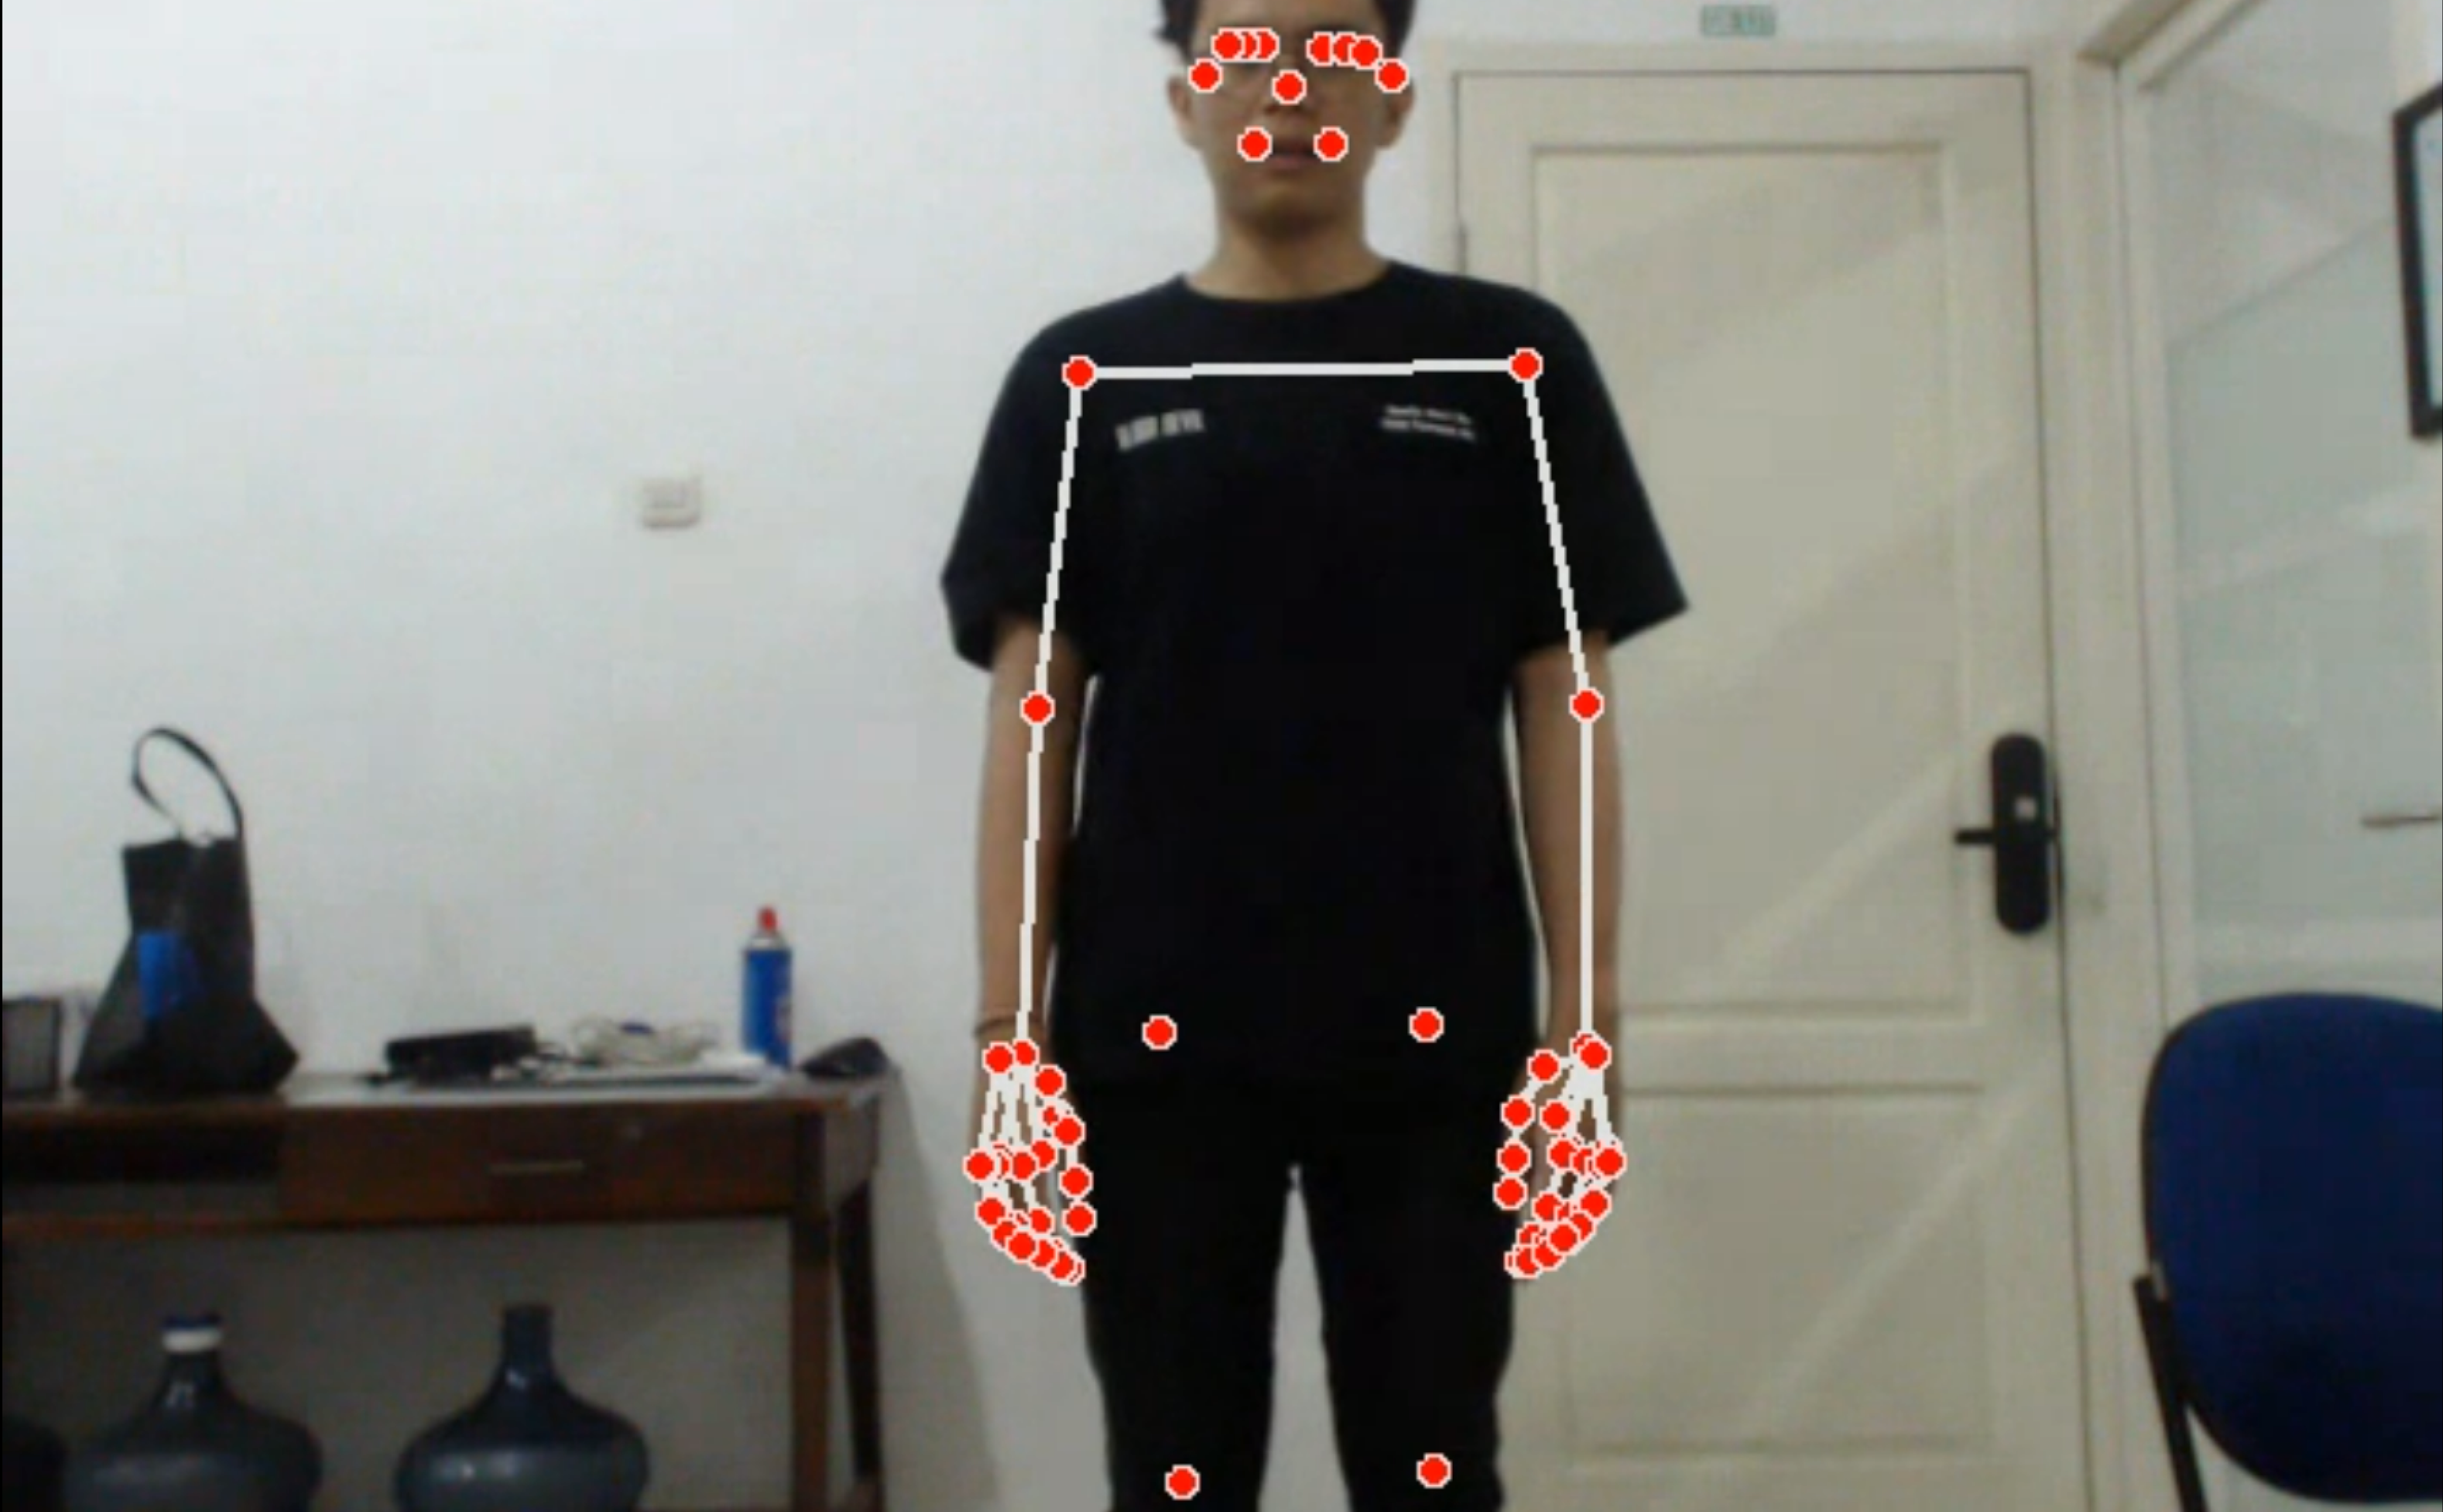
\includegraphics[scale=0.17]{gambar/bab4-jarak300.png}                \\
  \hline
  240 cm            & 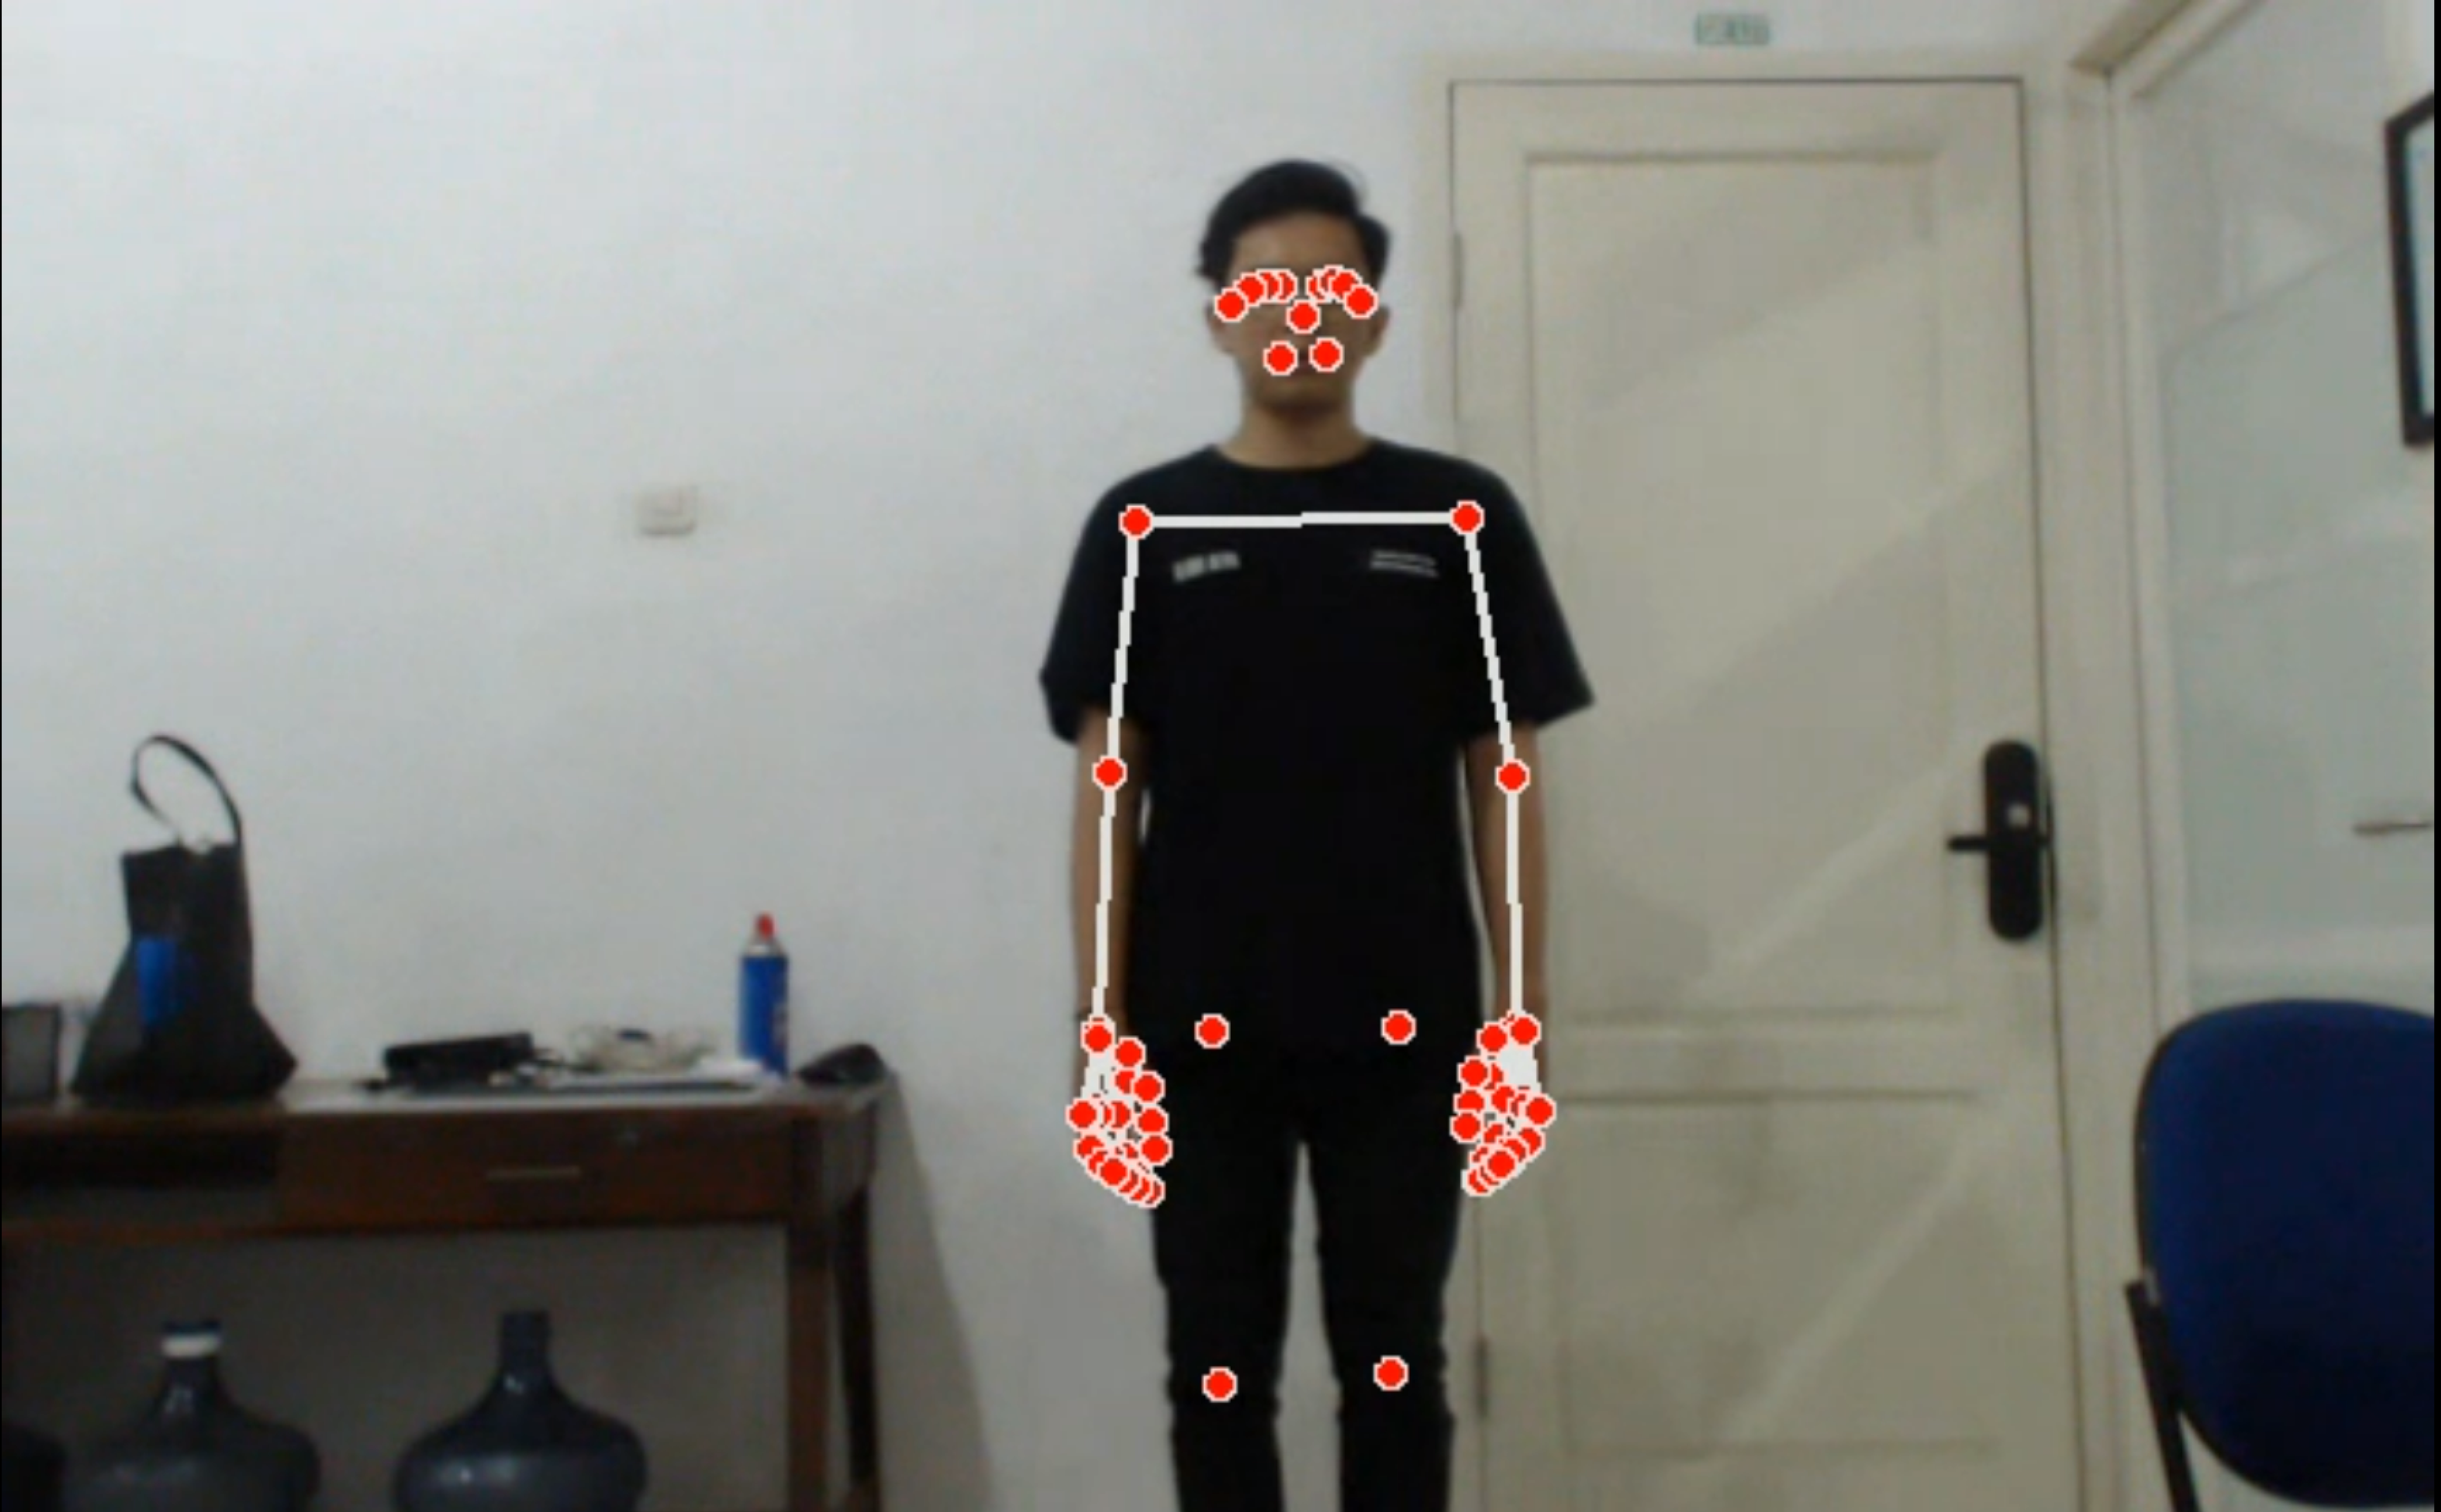
\includegraphics[scale=0.17]{gambar/bab4-jarak240.png}                 \\
  \hline
  300 cm            & 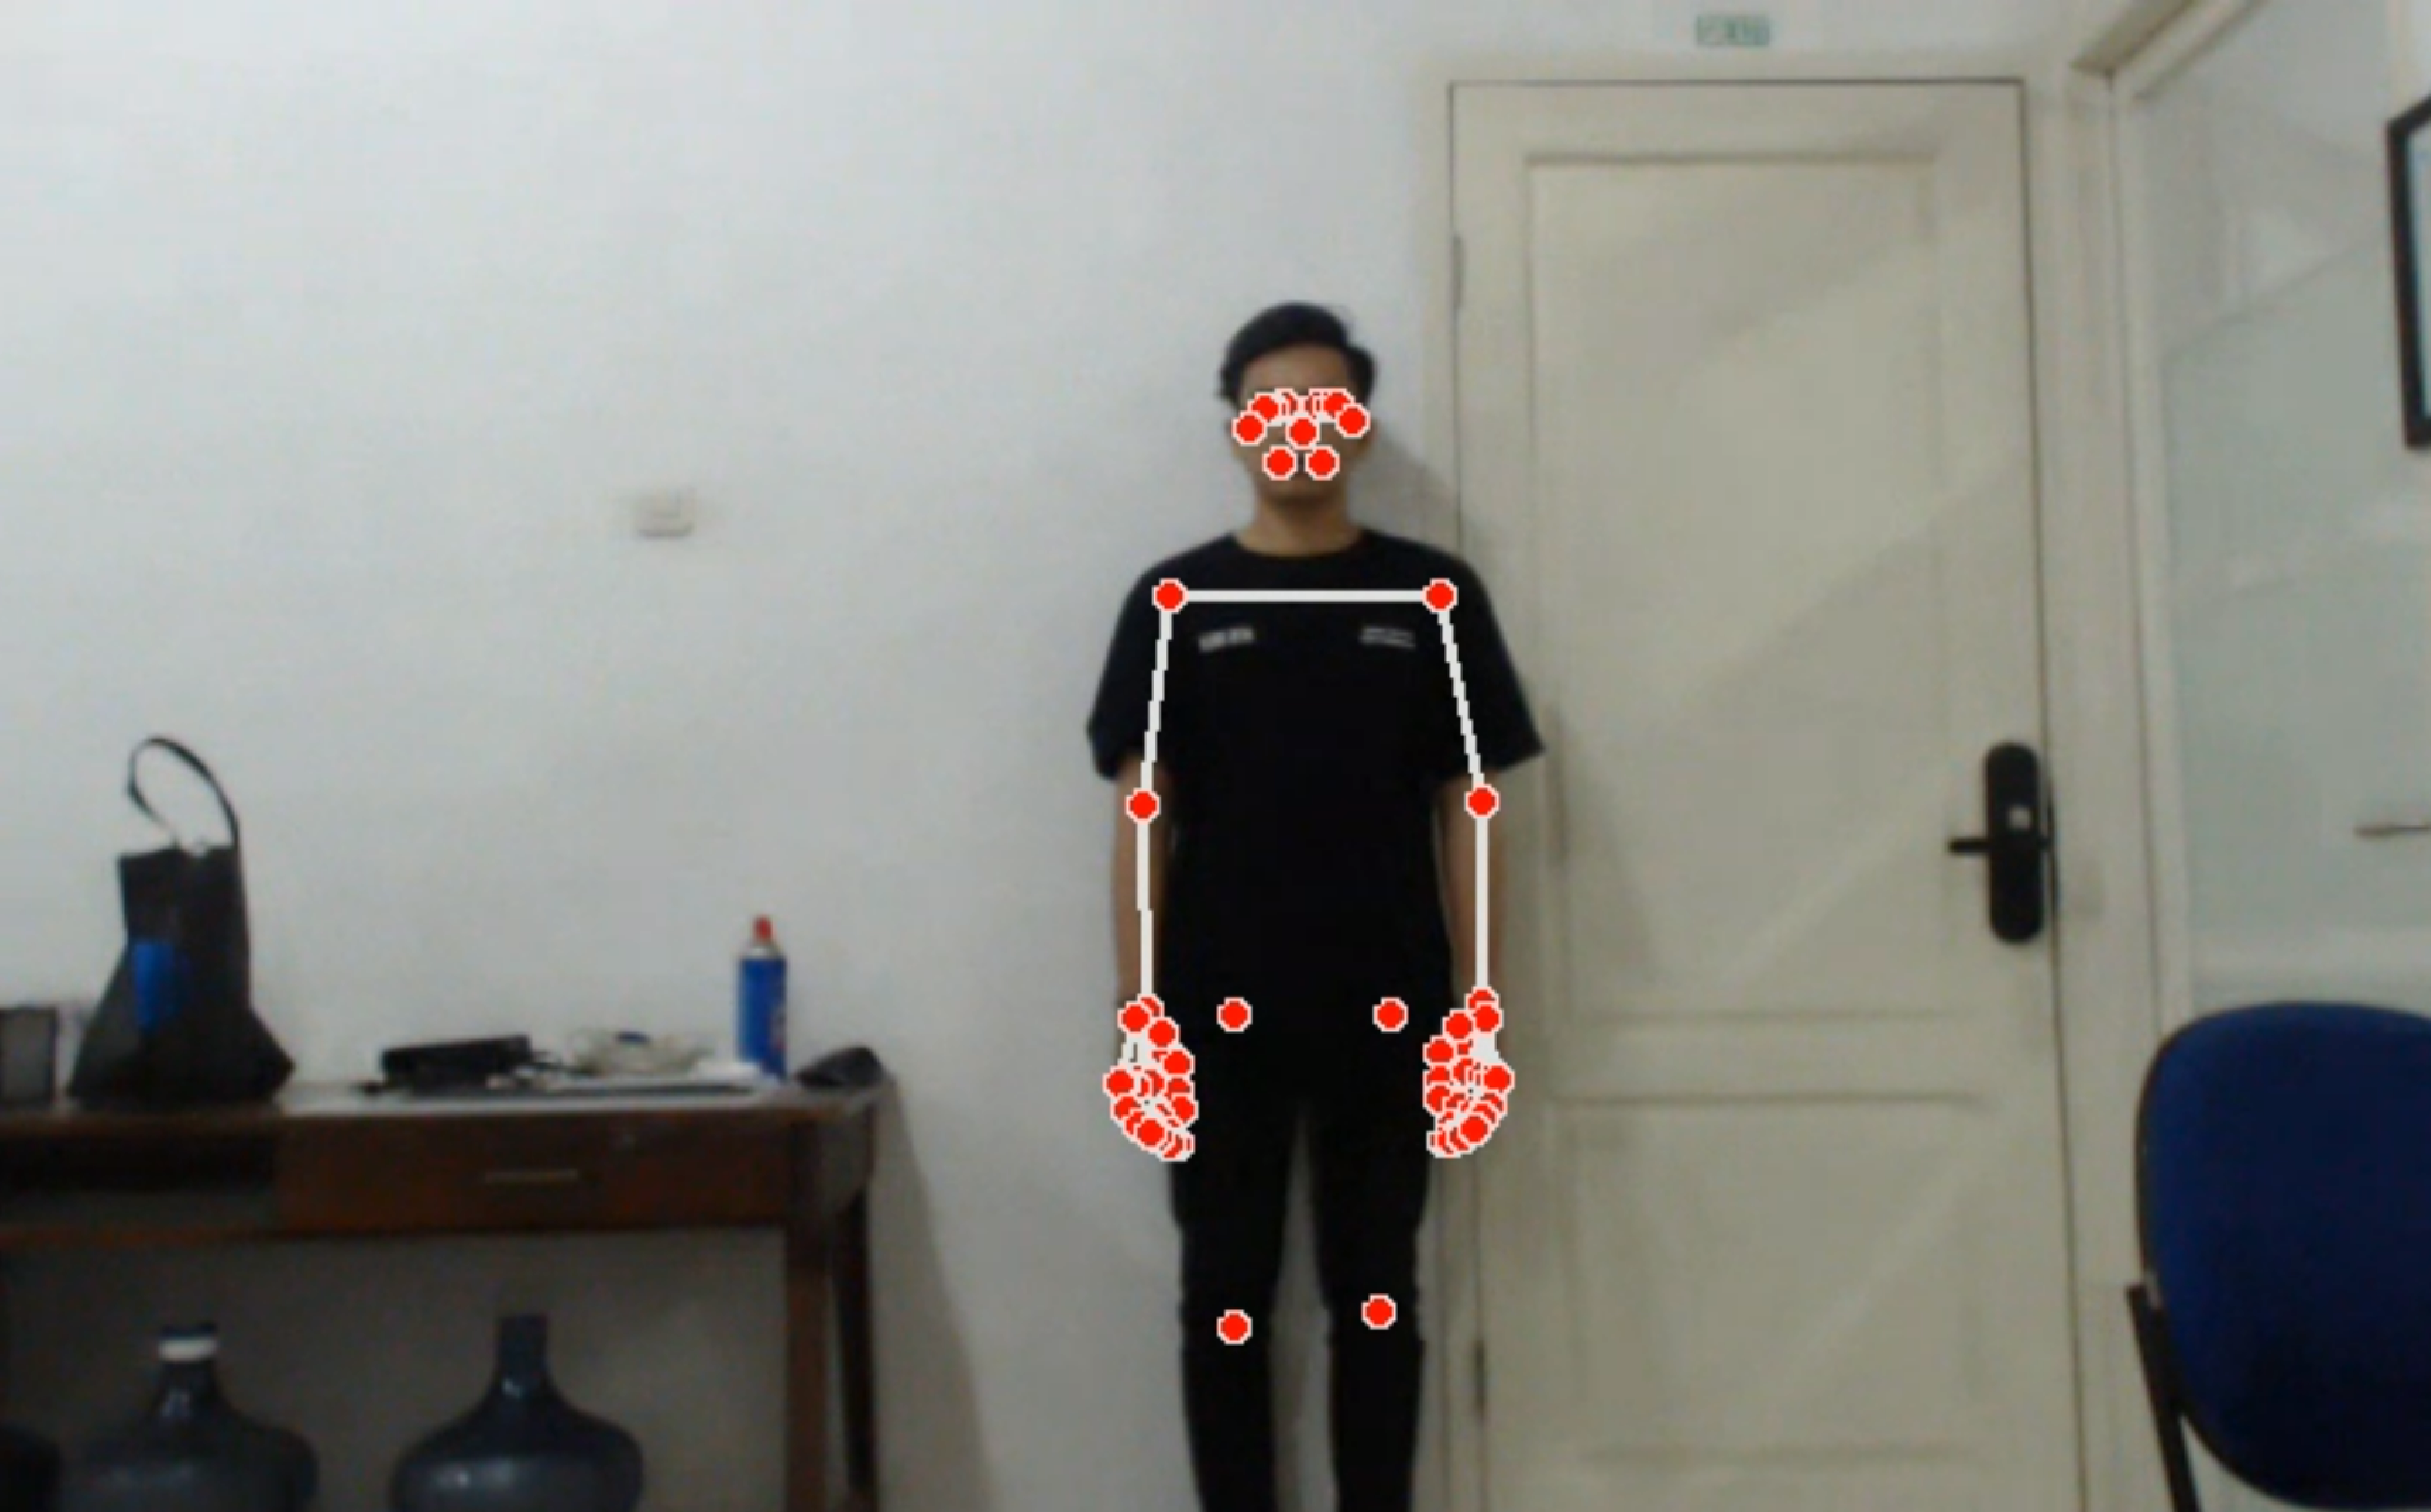
\includegraphics[scale=0.17]{gambar/bab4-jarak180.png}                 \\
  \hline
\end{longtable}

\newpage
\subsection{Pengujian Jarak 180 cm}
\label{sec:analisisjarak1}

\begin{longtable}{|c|c|c|c|c|}
  \caption{Pengujian Pertama Model di Kondisi Jarak 180 cm}
  \label{tb:prediksipendek1}                                   \\
  \hline
  \rowcolor[HTML]{C0C0C0}
  \textbf{Kosakata} & \textbf{Klasifikasi Model} & \textbf{\emph{Processing Time}} & \textbf{\emph{Complete Time}} & \textbf{\emph{FPS}}\\
  \hline
  Maaf              & Maaf                          & 0.09432 detik                           & 2.62625 detik                                 & 11.42311201\\
  Tolong            & Tolong                        & 0.09578 detik                           & 2.75824 detik                                 & 10.8764982\\
  Nama              & Nama                          & 0.09367 detik                           & 2.76423 detik                                 & 10.85294217\\
  Saya              & Saya                          & 0.09214 detik                           & 1.45957 detik                                 & 20.55396618\\
  Siapa             & Siapa                         & 0.09188 detik                           & 2.68606 detik                                 & 11.16875744\\
  Rumah             & \textcolor{red}{Delete}       & 0.09518 detik                           & 2.72404 detik                                 & 11.01303666\\
  Delete            & Delete                        & 0.09379 detik                           & 1.47150 detik                                 & 20.38732131\\
  Standby           & Standby                       & 0.09064 detik                           & 1.40810 detik                                 & 21.30526701\\
  Translate         & Translate                     & 0.09036 detik                           & 2.90195 detik                                 & 10.33787667\\
  \hline
\end{longtable}


\begin{longtable}{|c|c|c|c|c|}
  \caption{Pengujian Kedua Model di Kondisi Jarak 180 cm}
  \label{tb:prediksipendek2}                                   \\
  \hline
  \rowcolor[HTML]{C0C0C0}
  \textbf{Kosakata} & \textbf{Klasifikasi Model} & \textbf{\emph{Processing Time}} & \textbf{\emph{Complete Time}} & \textbf{\emph{FPS}}\\
  \hline
  Maaf              & \textcolor{red}{Tolong}       & 0.10251 detik                           & 2.68328 detik                                 & 11.18033853\\
  Tolong            & Tolong                        & 0.10531 detik                           & 2.67619 detik                                 & 11.20998081\\
  Nama              & Nama                          & 0.10347 detik                           & 2.83800 detik                                 & 10.57082874\\
  Saya              & Saya                          & 0.10078 detik                           & 1.60659 detik                                 & 18.67313694\\
  Siapa             & Siapa                         & 0.09793 detik                           & 2.89107 detik                                 & 10.37677789\\
  Rumah             & Rumah                         & 0.09961 detik                           & 2.97634 detik                                 & 10.07950553\\
  Delete            & Delete                        & 0.10204 detik                           & 1.43186 detik                                 & 20.95172062\\
  Standby           & Standby                       & 0.10917 detik                           & 1.42540 detik                                 & 21.04676217\\
  Translate         & Translate                     & 0.10983 detik                           & 3.00642 detik                                 & 9.978645248\\
  \hline
\end{longtable}


\begin{longtable}{|c|c|c|c|c|}
  \caption{Pengujian Ketiga Model di Kondisi Jarak 180 cm}
  \label{tb:prediksipendek3}                                   \\
  \hline
  \rowcolor[HTML]{C0C0C0}
  \textbf{Kosakata} & \textbf{Klasifikasi Model} & \textbf{\emph{Processing Time}} & \textbf{\emph{Complete Time}} & \textbf{\emph{FPS}}\\
  \hline
  Maaf              & Maaf                          & 0.09704 detik                           & 2.60797 detik                                 & 11.50321979\\
  Tolong            & Tolong                        & 0.11110 detik                           & 2.68802 detik                                 & 11.16064415\\
  Nama              & Nama                          & 0.11300 detik                           & 2.85448 detik                                 & 10.50980117\\
  Saya              & Saya                          & 0.10576 detik                           & 1.40619 detik                                 & 21.33420142\\
  Siapa             & Siapa                         & 0.10793 detik                           & 2.81908 detik                                 & 10.64176832\\
  Rumah             & Rumah                         & 0.10235 detik                           & 2.89943 detik                                 & 10.34685349\\
  Delete            & Delete                        & 0.10875 detik                           & 1.38759 detik                                 & 21.62023516\\
  Standby           & Standby                       & 0.11035 detik                           & 1.39657 detik                                 & 21.48127055\\
  Translate         & Translate                     & 0.10169 detik                           & 3.11065 detik                                 & 9.644273064\\
  \hline
\end{longtable}


Berdasarkan tiga pengujian yang dilakukan, didapatkan bahwa hampir keseluruhan klasifikasi model yang sesuai dengan \emph{class} kosakata. Namun, terdapat beberapa kesalahan model dalam melakukan klasifikasi. Dapat dilihat pada tabel \ref{tb:prediksipendek1} untuk isyarat kosakata "Rumah" diklasifikasikan sebagai "Delete" dan pada tabel \ref{tb:prediksipendek2} untuk isyarat kosakata "Maaf" diklasifikasikan sebagai "Tolong". Adanya kemiripan antara kosakata menjadi penyebab utama terjadinya kesalahan ini. Kosakata "Rumah" dan "Delete" memiliki kemiripan pada gerakan isyaratnya, dimana kedua kosakata ini sama - sama menggunakan dua tangan dengan gerakan yang mayoritas terjadi pada bagian badan pengguna. Sedangkan untuk kosakata "Maaf" dan "Tolong" memiliki kemiripan pada gerakan isyaratnya dengan kedua kosakata sama - sama menggunakan tangan kanan dengan gerakan akhir yang mayoritas terjadi pada bagian samping wajah pengguna. Namun kemiripan ini tidak sepenuhnya membuat hasil klasifikasi menjadi lebih condong ke suatu kosakata, melainkan dengan pengguna yang memperagakan bahasa isyarat dengan mengutamakan "ciri khas" dari masing - masing bahasa isyarat dapat menghasilkan hasil klasifikasi model yang baik. Hal ini dapat dilihat pada tabel \ref{tb:prediksipendek2} menghasilkan keseluruhan klasifikasi yang benar untuk seluruh \emph{class} kosakata. Pada pengujian dengan kondisi jarak 180 cm, berdasarkan data pda tabel \ref{tb:prediksipendek1}, tabel tabel \ref{tb:prediksipendek2}, dan tabel tabel \ref{tb:prediksipendek3} menunjukkan bahwa model memiliki akurasi klasifikasi sebesar 92.5\%.

Apabila dilihat berdasarkan waktu pemrosesan, rata - rata waktu yang dibutuhkan model untuk menghasilkan klasifikasi bahasa isyarat (\emph{processing time}) adalah 0.101 detik dan rata - rata waktu yang dibutuhkan dalam menghasilkan klasifikasi bahasa isyarat (\emph{complete time}) adalah 2.352 detik. Berdasakan data ini, dapat diamati bahwa model memerlukan waktu yang terbilang singkat dalam memproses serangkaian data koordinat yang diberikan dengan program penerjemah yang mampu menyelesaikan proses klasifikasi dengan cepat untuk sistem yang berjalan secara \emph{real time}. Adapun untuk nilai rata - rata FPS berdasarkan 3 pengujian yang dilakukan adalah 14.083. Meskipun dengan kondisi pengguna yang memiliki jarak yang cukup dekat dengan kamera, tidak mempengaruhi secara signifikan terhadap proses klasifikasi bahasa isyarat yang dilakukan oleh model.

Pada pengujian di kondisi jarak 180 cm ini, perlu diperhatikan bahwa pengguna harus melakukan gerakan bahasa isyarat dengan memastikan bahwa bagian tubuh kepala hingga tangan dengan jelas terlihat. Hal ini sangat krusial karena model memerlukan informasi koordinat yang lengkap untuk setiapp gerakan isyarat sehingga dapat menghasilkan klasifikasi yang tepat. Terkhususnya untuk kosakata "Translate", "Maaf", "Tolong", dan "Delete" yang memiliki gerakan isyarat yang cukup dinamis dan mayoritas gerakannya terjadi di samping kepala pengguna.  

\subsection{Pengujian Jarak 240 cm}
\label{sec:analisisjarak2}

\begin{longtable}{|c|c|c|c|c|}
  \caption{Pengujian Pertama Model di Kondisi Jarak 240 cm}
  \label{tb:prediksitengah1}                                   \\
  \hline
  \rowcolor[HTML]{C0C0C0}
  \textbf{Kosakata} & \textbf{Klasifikasi Model} & \textbf{\emph{Processing Time}} & \textbf{\emph{Complete Time}} & \textbf{\emph{FPS}}\\
  \hline
  Maaf              & Maaf                          & 0.09363 detik                           & 2.86369 detik                                  & 10.47599114\\
  Tolong            & Tolong                        & 0.09594 detik                           & 2.69973 detik                                  & 11.11221089\\
  Nama              & Nama                          & 0.09915 detik                           & 2.71606 detik                                  & 11.04540295\\
  Saya              & Saya                          & 0.09490 detik                           & 1.38486 detik                                  & 21.66277929\\
  Siapa             & Siapa                         & 0.09771 detik                           & 2.77829 detik                                  & 10.7980115\\
  Rumah             & Rumah                         & 0.09179 detik                           & 2.84222 detik                                  & 10.55513362\\
  Delete            & Delete                        & 0.09783 detik                           & 2.74689 detik                                  & 10.92144369\\
  Standby           & Standby                       & 0.09716 detik                           & 1.44449 detik                                  & 20.76861067\\
  Translate         & Translate                     & 0.09462 detik                           & 2.89943 detik                                  & 10.34685349\\
  \hline
\end{longtable}


\newpage
\begin{longtable}{|c|c|c|c|c|}
  \caption{Pengujian Kedua Model di Kondisi Jarak 240 cm}
  \label{tb:prediksitengah2}                                   \\
  \hline
  \rowcolor[HTML]{C0C0C0}
  \textbf{Kosakata} & \textbf{Klasifikasi Model} & \textbf{\emph{Processing Time}} & \textbf{\emph{Complete Time}} & \textbf{\emph{FPS}}\\
  \hline
  Maaf              & Maaf                          & 0.10063 detik                           & 2.83704 detik                                  & 10.57439991\\
  Tolong            & Tolong                        & 0.10465 detik                           & 2.74551 detik                                  & 10.926935\\
  Nama              & Nama                          & 0.07916 detik                           & 2.71480 detik                                  & 11.0505538\\
  Saya              & Saya                          & 0.11030 detik                           & 1.45698 detik                                  & 20.59049293\\
  Siapa             & Siapa                         & 0.09941 detik                           & 2.71764 detik                                  & 11.0389784\\
  Rumah             & Rumah                         & 0.10740 detik                           & 2.78343 detik                                  & 10.77806101\\
  Delete            & Delete                        & 0.10263 detik                           & 2.84822 detik                                  & 10.5328947\\
  Standby           & Standby                       & 0.10418 detik                           & 1.42558 detik                                  & 21.04412222\\
  Translate         & Translate                     & 0.10815 detik                           & 2.91372 detik                                  & 10.29610573\\
  \hline
\end{longtable}



\begin{longtable}{|c|c|c|c|c|}
  \caption{Pengujian Ketiga Model di Kondisi Jarak 240 cm}
  \label{tb:prediksitengah3}                                   \\
  \hline
  \rowcolor[HTML]{C0C0C0}
  \textbf{Kosakata} & \textbf{Klasifikasi Model} & \textbf{\emph{Processing Time}} & \textbf{\emph{Complete Time}} & \textbf{\emph{FPS}}\\
  \hline
  Maaf              & Maaf                          & 0.08161 detik                           & 2.93442 detik                                  & 10.22350162\\
  Tolong            & Tolong                        & 0.10857 detik                           & 2.84241 detik                                  & 10.55441648\\
  Nama              & Nama                          & 0.08474 detik                           & 2.87571 detik                                  & 10.43221665\\
  Saya              & Saya                          & 0.10568 detik                           & 1.77221 detik                                  & 16.92801072\\
  Siapa             & Siapa                         & 0.10201 detik                           & 2.62119 detik                                  & 11.4451809\\
  Rumah             & \textcolor{red}{Delete}       & 0.10468 detik                           & 2.72556 detik                                  & 11.00690965\\
  Delete            & Delete                        & 0.10309 detik                           & 2.82816 detik                                  & 10.60758815\\
  Standby           & Standby                       & 0.10799 detik                           & 1.42754 detik                                  & 21.01512639\\
  Translate         & Translate                     & 0.10627 detik                           & 2.81355 detik                                  & 10.66268053\\
  \hline
\end{longtable}




Berdasarkan tiga pengujian yang telah dilakukan, didapatkan bahwa hampir keseluruhan klasifikasi model telah sesuai dengan \emph{class} kosakata yang bersesuaian. Hal ini menunjukkan bahwa adanya pengaruh antara jarak pengguna dengan kamera terhadap proses klasifikasi model. Peningkatan jarak pengguna terhadap menghasilkan klasifikasi yang lebih baik. Namun, masih terdapat kesalahan yang dapat dilihat pada tabel \ref{tb:prediksitengah3}, yaitu isyarat kosakata "Rumah" diklasifikasikan sebagai "Delete". Sama seperti yang sudah dijelaskan pada pengujian di kondisi jarak 180 cm bahwa terdapat kemiripan antara kosakata "Rumah" dengan "Delete". Pada pengujian dengan kondisi jarak 240 cm ini, berdasarkan data pada tabel \ref{tb:prediksitengah1}, tabel \ref{tb:prediksitengah2}, dan tabel \ref{tb:prediksitengah3} menunjukkan bahwa model memiliki akurasi klasifikasi sebesar 96.3\%.

Apabila dilihat berdasarkan waktu pemrosesan, rata - rata waktu yang dibutuhkan model untuk menghasilkan klasifikasi bahasa isyarat (\emph{processing time}) adalah 0.099 detik dan rata - rata waktu yang dibutuhkan dalam menghasilkan klasifikasi bahasa isyarat (\emph{complete time}) adalah 2.506 detik. Apabila dibandingkan dengan pengujian sebelumnya (kondisi jarak 180 cm). Terdapat peningkatan pada nilai \emph{processing time} seiring dengan peningkatan jarak kamera dengan pengguna yaitu sebesar 0.002 detik. Sedangkan untuk nilai \emph{complete time} mengalami penurunan seiring dengan peningkatan jarak kamera dengan pengguna, yaitu sebesar 0.154 detik. Adapun rata - rata FPS yang didapatkan bernilai 12.866. Apabila dilihat dari pengujian sebelumnya, terdapat penurunan dari nilai rata - rata FPS ini. Hal ini dapat disebabkan oleh adanya pengaruh antara jarak pengguna dengan kamera terhadap bagaimana beban kerja kamera dalam menangkap tiap \emph{frame}.

\subsection{Pengujian Jarak 300 cm}
\label{sec:analisisjarak3}

\begin{longtable}{|c|c|c|c|c|}
  \caption{Pengujian Pertama Model di Kondisi Jarak 300 cm}
  \label{tb:prediksijauh1}                                   \\
  \hline
  \rowcolor[HTML]{C0C0C0}
  \textbf{Kosakata} & \textbf{Klasifikasi Model} & \textbf{\emph{Processing Time}} & \textbf{\emph{Complete Time}} & \textbf{\emph{FPS}}\\
  \hline
  Maaf              & Maaf                          & 0.09520 detik                           & 2.73861 detik                                  & 10.95444597\\
  Tolong            & Tolong                        & 0.09268 detik                           & 2.87873 detik                                  & 10.42125245\\
  Nama              & Nama                          & 0.09824 detik                           & 2.91580 detik                                  & 10.28878128\\
  Saya              & Saya                          & 0.09438 detik                           & 2.81194 detik                                  & 10.66878297\\
  Siapa             & Siapa                         & 0.10269 detik                           & 2.76496 detik                                  & 10.85005044\\
  Rumah             & Rumah                         & 0.09520 detik                           & 2.74032 detik                                  & 10.9476124\\
  Delete            & Delete                        & 0.09270 detik                           & 2.98108 detik                                  & 10.06347157\\
  Standby           & Standby                       & 0.09150 detik                           & 2.81312 detik                                  & 10.66433428\\
  Translate         & Translate                     & 0.09415 detik                           & 2.84808 detik                                  & 10.53339729\\
  \hline
\end{longtable}


\begin{longtable}{|c|c|c|c|c|}
  \caption{Pengujian Kedua Model di Kondisi Jarak 300 cm}
  \label{tb:prediksijauh2}                                   \\
  \hline
  \rowcolor[HTML]{C0C0C0}
  \textbf{Kosakata} & \textbf{Klasifikasi Model} & \textbf{\emph{Processing Time}} & \textbf{\emph{Complete Time}} & \textbf{\emph{FPS}}\\
  \hline
  Maaf              & Maaf                          & 0.11375 detik                           & 2.86339 detik                                  & 10.47709021\\
  Tolong            & Tolong                        & 0.10336 detik                           & 2.74577 detik                                  & 10.92588184\\
  Nama              & Nama                          & 0.10118 detik                           & 2.69010 detik                                  & 11.15200889\\
  Saya              & Saya                          & 0.11127 detik                           & 2.72032 detik                                  & 11.02812309\\
  Siapa             & Siapa                         & 0.10363 detik                           & 2.84954 detik                                  & 10.52800361\\
  Rumah             & Rumah                         & 0.10374 detik                           & 2.87114 detik                                  & 10.44879738\\
  Delete            & Delete                        & 0.10743 detik                           & 2.73295 detik                                  & 10.97715222\\
  Standby           & Standby                       & 0.10061 detik                           & 2.90372 detik                                  & 10.33158689\\
  Translate         & Translate                     & 0.10337 detik                           & 2.75235 detik                                  & 10.89978846\\
  \hline
\end{longtable}


\begin{longtable}{|c|c|c|c|c|}
  \caption{Pengujian Ketiga Model di Kondisi Jarak 300 cm}
  \label{tb:prediksijauh3}                                   \\
  \hline
  \rowcolor[HTML]{C0C0C0}
  \textbf{Kosakata} & \textbf{Klasifikasi Model} & \textbf{\emph{Processing Time}} & \textbf{\emph{Complete Time}} & \textbf{\emph{FPS}}\\
  \hline
  Maaf              & Maaf                          & 0.09520 detik                           & 2.75798 detik                                  & 10.87754186\\
  Tolong            & Tolong                        & 0.09268 detik                           & 2.66197 detik                                  & 11.26986055\\
  Nama              & Nama                          & 0.09824 detik                           & 2.88613 detik                                  & 10.39454784\\
  Saya              & Saya                          & 0.09438 detik                           & 2.80015 detik                                  & 10.7137212\\
  Siapa             & Siapa                         & 0.10269 detik                           & 2.76350 detik                                  & 10.85577924\\
  Rumah             & Rumah                          & 0.09520 detik                           & 2.81146 detik                                  & 10.67060149\\
  Delete            & Delete                        & 0.09270 detik                           & 2.69894 detik                                  & 11.11547971\\
  Standby           & Standby                       & 0.09675 detik                           & 2.75581 detik                                  & 10.88609619\\
  Translate         & Translate                     & 0.10323 detik                           & 2.67942 detik                                  & 11.19645498\\
  \hline
\end{longtable}



Berdasarkan tiga pengujian yang telah dilakukan, didapatkan bahwa keseluruhan klasifikasi model yang sesuai dengan \emph{class} kosakata. Hal ini menunjukkan bahwa peningkatan jarak berpengaruh pada proses klasifikasi yang dilakukan oleh model. Peningkatan jarak antara pengguna dengan kamera, terkhususnya pada jarak terjauh pada pengujian ini, menghasilkan klasifikasi yang lebih baik dan tepat sesuai dengan kosakata yang bersesuaian dengan gerakannya. Hal ini dapat disebabkan oleh semakin jauh jarak antara kamera dengan pengguna memudahkan dalam memproses pose pengguna sehingga menghasilkan data koordinat yang lebih baik lagi. Berdasarkan data pada tabel \ref{tb:prediksijauh1}, tabel \ref{tb:prediksijauh2}, tabel \ref{tb:prediksijauh3} menunjukkan bahwa model memiliki akurasi klasifikasi sebesar 100\%.

Apabila dilihat berdasarkan waktu pemrosesan, rata - rata waktu yang dibutuhkan model untuk menghasilkan klasifikasi bahasa isyarat (\emph{processing time}) adalah 0.099 detik dan rata - rata waktu yang dibutuhkan dalam menghasilkan klasifikasi bahasa isyarat (\emph{complete time}) adalah 2.794 detik. Dapat dilihat bahwa tidak terdapat peningkatan pada \emph{processing time} jika dibandingkan dengan variasi jarak pada pengujian sebelumnya. Namun, pada nilai \emph{complete time} terdapat penurunan jika dibandingkan dengan pengujian sebelumnya, yaitu sebesar 0.288 detik. Hal ini menunjukkan bahwa terdapat penurunan dari nilai \emph{complete time} seiring dengan peningkatan jarak kamera dengan pengguna. Adapun untuk nilai rata - rata FPS yang didapatkan berdasarkan 3 pengujian yang telah dilakukan bernilai 10.746. Apabila dibandingkan dengan pengujian - pengujian sebelumnya, terdapat penurunan pada nilai rata - rata FPS ini. Hal ini dapat kembali lagi menguatkan bahwa adanya pengaruh antara jarak pengguna dengan kamera terhadap bagaimana beban kerja kamera dalam menangkap tiap \emph{frame}, dimana adanya peningkatan jarak menghasilkan model yang lebih baik dalam melakukan klasifikasi, namun dengan beban kerja yang lebih berat bagi sistem secara keseluruhan.

\subsection{Rangkuman Pengujian Kondisi Jarak}
\label{sec:analisisrangkumanjarak}

\begin{longtable}{|c|c|c|c|c|}
  \caption{Rangkuman Pengujian Kondisi Jarak}
  \label{tb:evaluasiJarak}                                   \\
  \hline
  \rowcolor[HTML]{C0C0C0}
  \textbf{Jarak} & \textbf{Akurasi} & \emph{\textbf{Avg. Processing Time}} & \emph{\textbf{Avg. Complete Time}} & \emph{FPS}\\
  \hline
  180 cm & 0.89 & 0.1017 detik & 2.3660 detik & 14.083\\
  240 cm & 0.96 & 0.0994 detik & 2.5098 detik & 12.866\\
  300 cm & 1.00 & 0.0997 detik & 2.7918 detik & 10.746\\
  \hline
\end{longtable}

Secara keseluruhan, dapat dilihat pada tabel \ref{tb:evaluasiJarak} bahwa variasi jarak yang berbeda tidak berpengaruh secara signifikan terhadap hasil klasifikasi model. Hal ini menunjukkan bahwa metode normalisasi data yang digunakan telah berhasil menghasilkan model yang invarian terhadap jarak. Dengan catatan bahwa posisi pengguna (terkhususnya bagian kepala dan tangan) dapat dengan jelas terlihat ketika melakukan gerakan isyarat. Dapat dilihat bahwa ada relasi antara jarak dengan \emph{average complete time}. Peningkatan \emph{average}. Namun, pada nilai \emph{average processing time} cenderung menurun dengan adanya peningkatan jarak. Kemampuan kamera dalam menangkap \emph{frame} menjadi pengaruh utama dalam peningkatan nilai \emph{complete time} dan \emph{processing time} karena gerakan isyarat yang dinamis memerlukan posisi kamera yang dapat menangkap setiap gerakan dengan jelas dan tepat. Semakin jelas gerakan isyarat yang ditangkap akan memudahkan \emph{framework} Mediapipe dalam mendapatkan data koordinat berdasarkan \emph{landmark} yang ada. Hal ini tentunya akan meningkatkan akurasi klasifikasi model, dimana ditunjukkan dengan adanya peningkatan akurasi seiring dengan peningkatan jarak. Adapun pada nilai rata - rata FPS mengalami penurunan seiring dengan peningkatan jarak antara pengguna dengan kamera. Hal ini menunjukkan bahwa sistem memiliki beban kerja yang lebih berat seiring dengan peningkatan jarak.

\newpage
\section{Pengujian Subjek Berbeda}
\label{sec:analisissubjek}

\begin{longtable}{|c|c|}
  \caption{Variasi Subjek Berbeda}
  \label{tb:kondisisubjek}                                   \\
  \hline
  \rowcolor[HTML]{C0C0C0}
  \textbf{Jenis Kelamin} & \textbf{Gambar Subjek}  \\
  \hline
  Perempuan              &  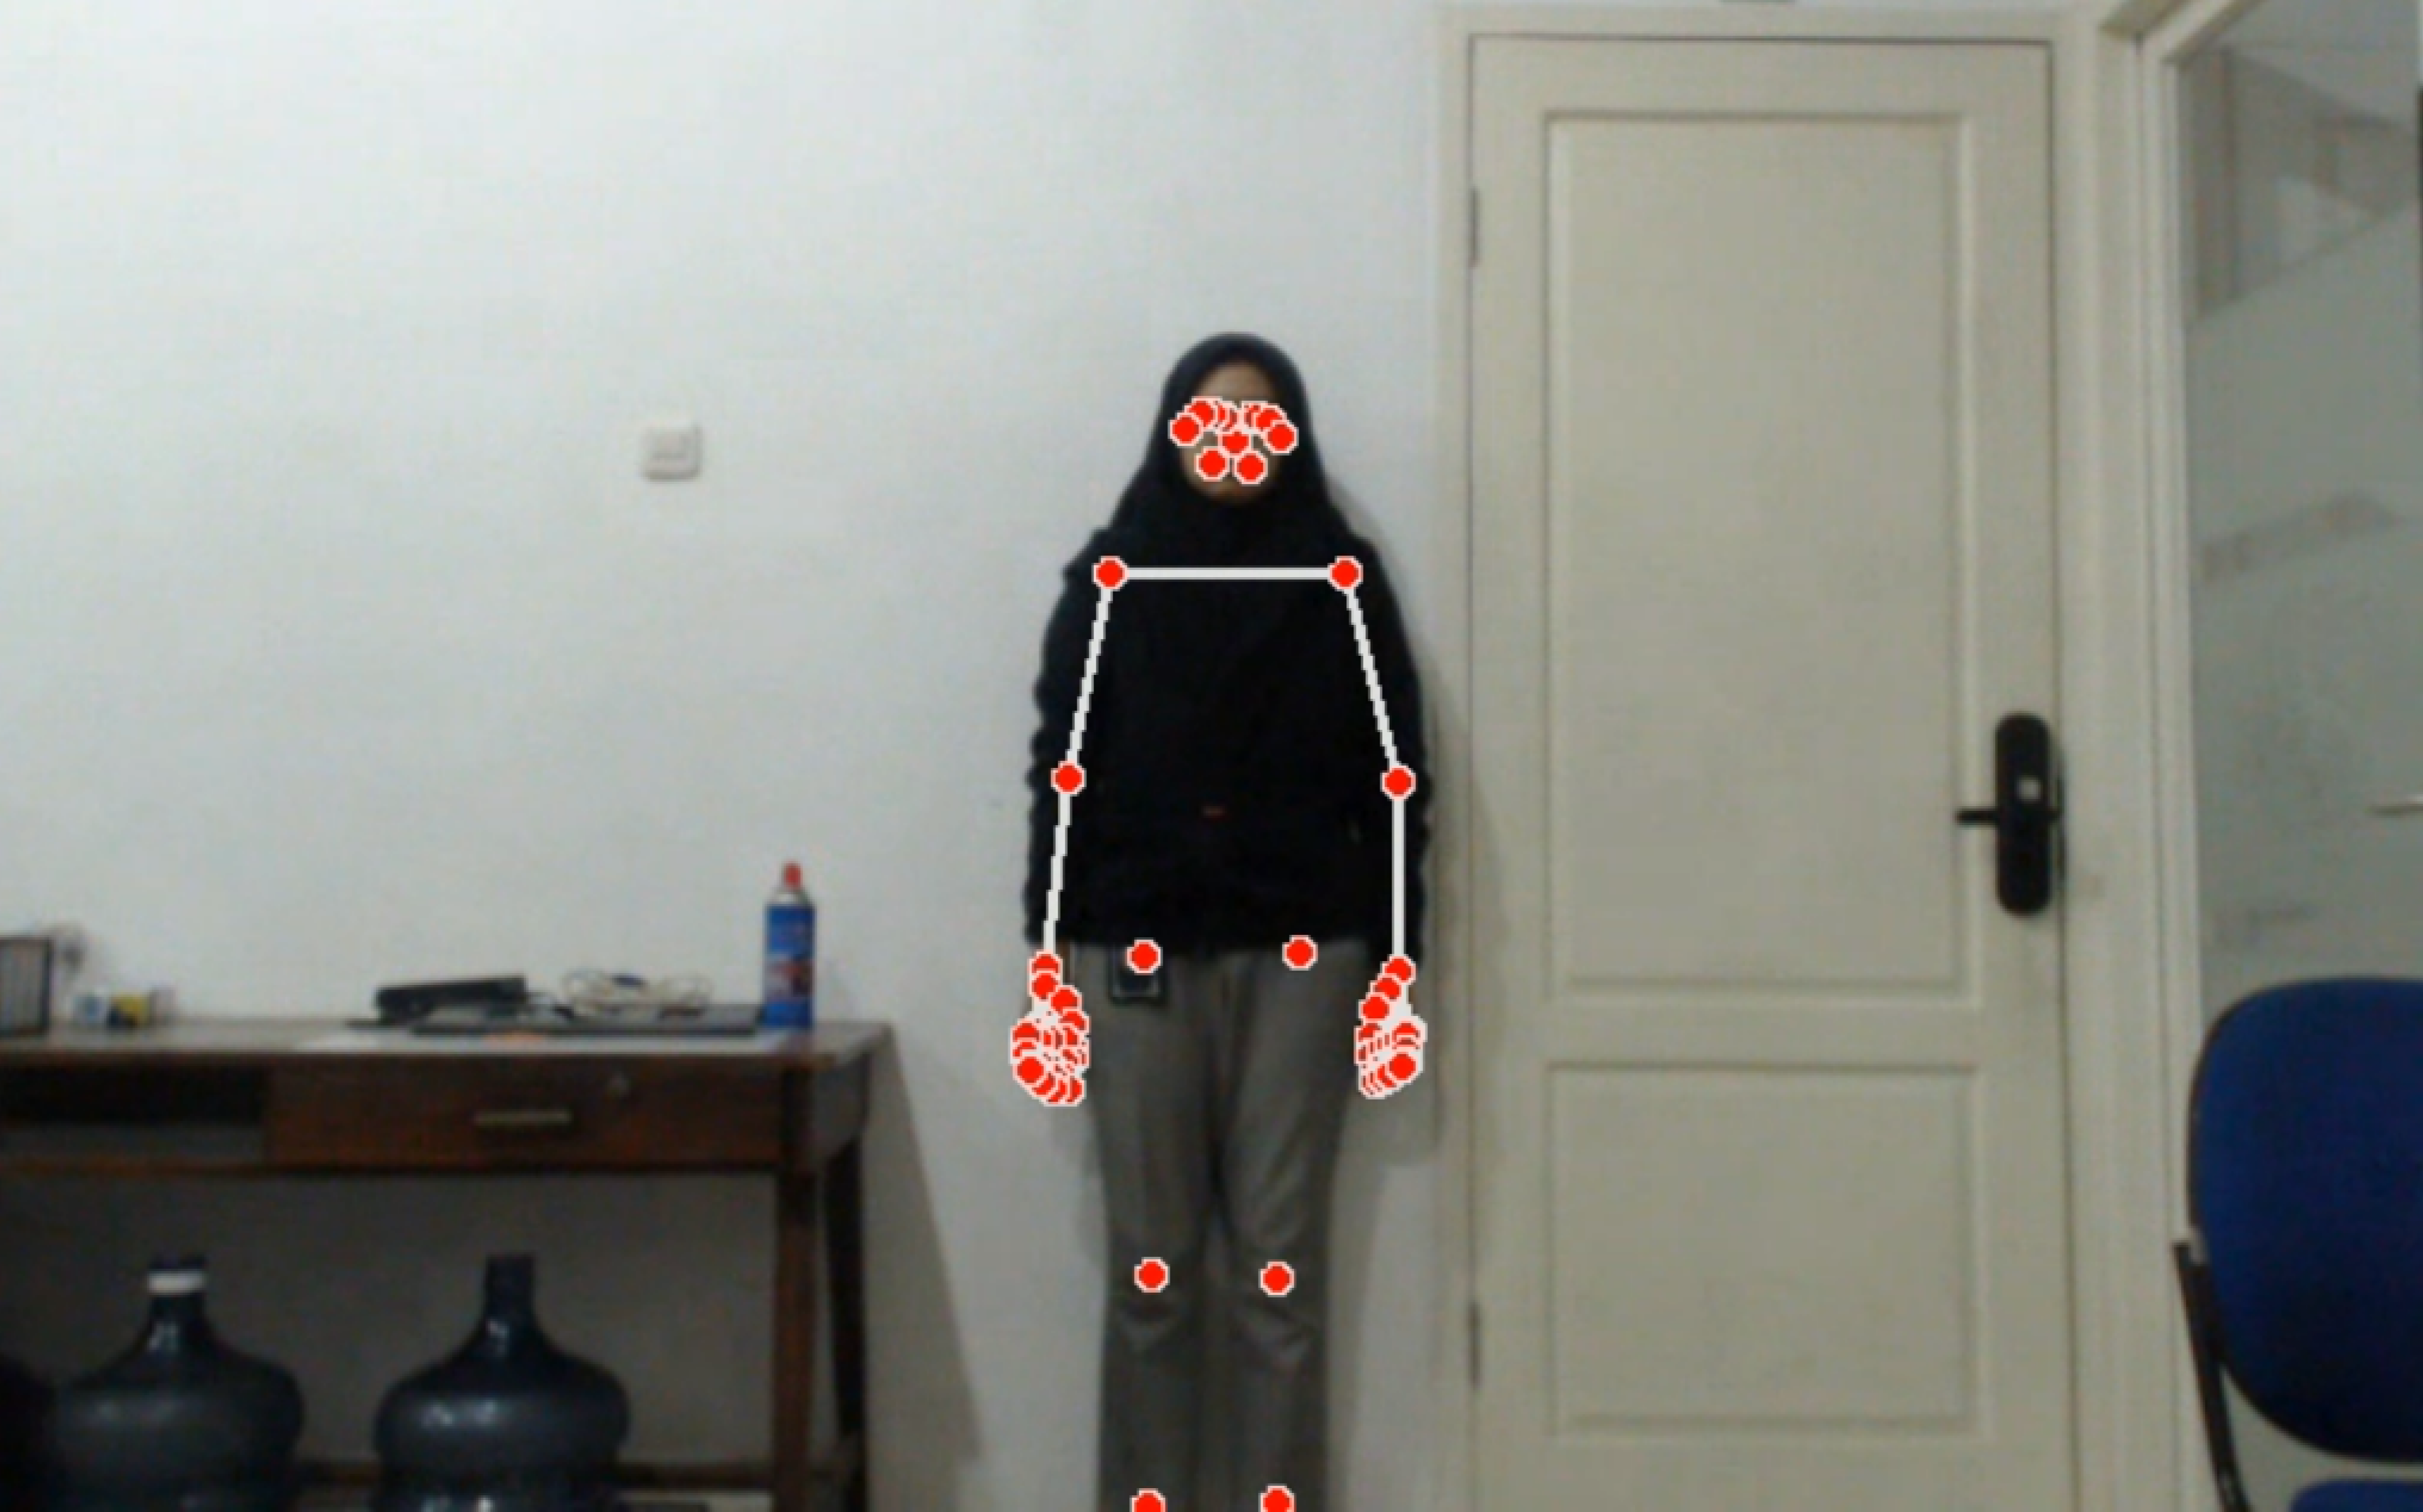
\includegraphics[scale=0.3]{gambar/bab4-rani.png}                \\
  \hline
  Laki - Laki            & 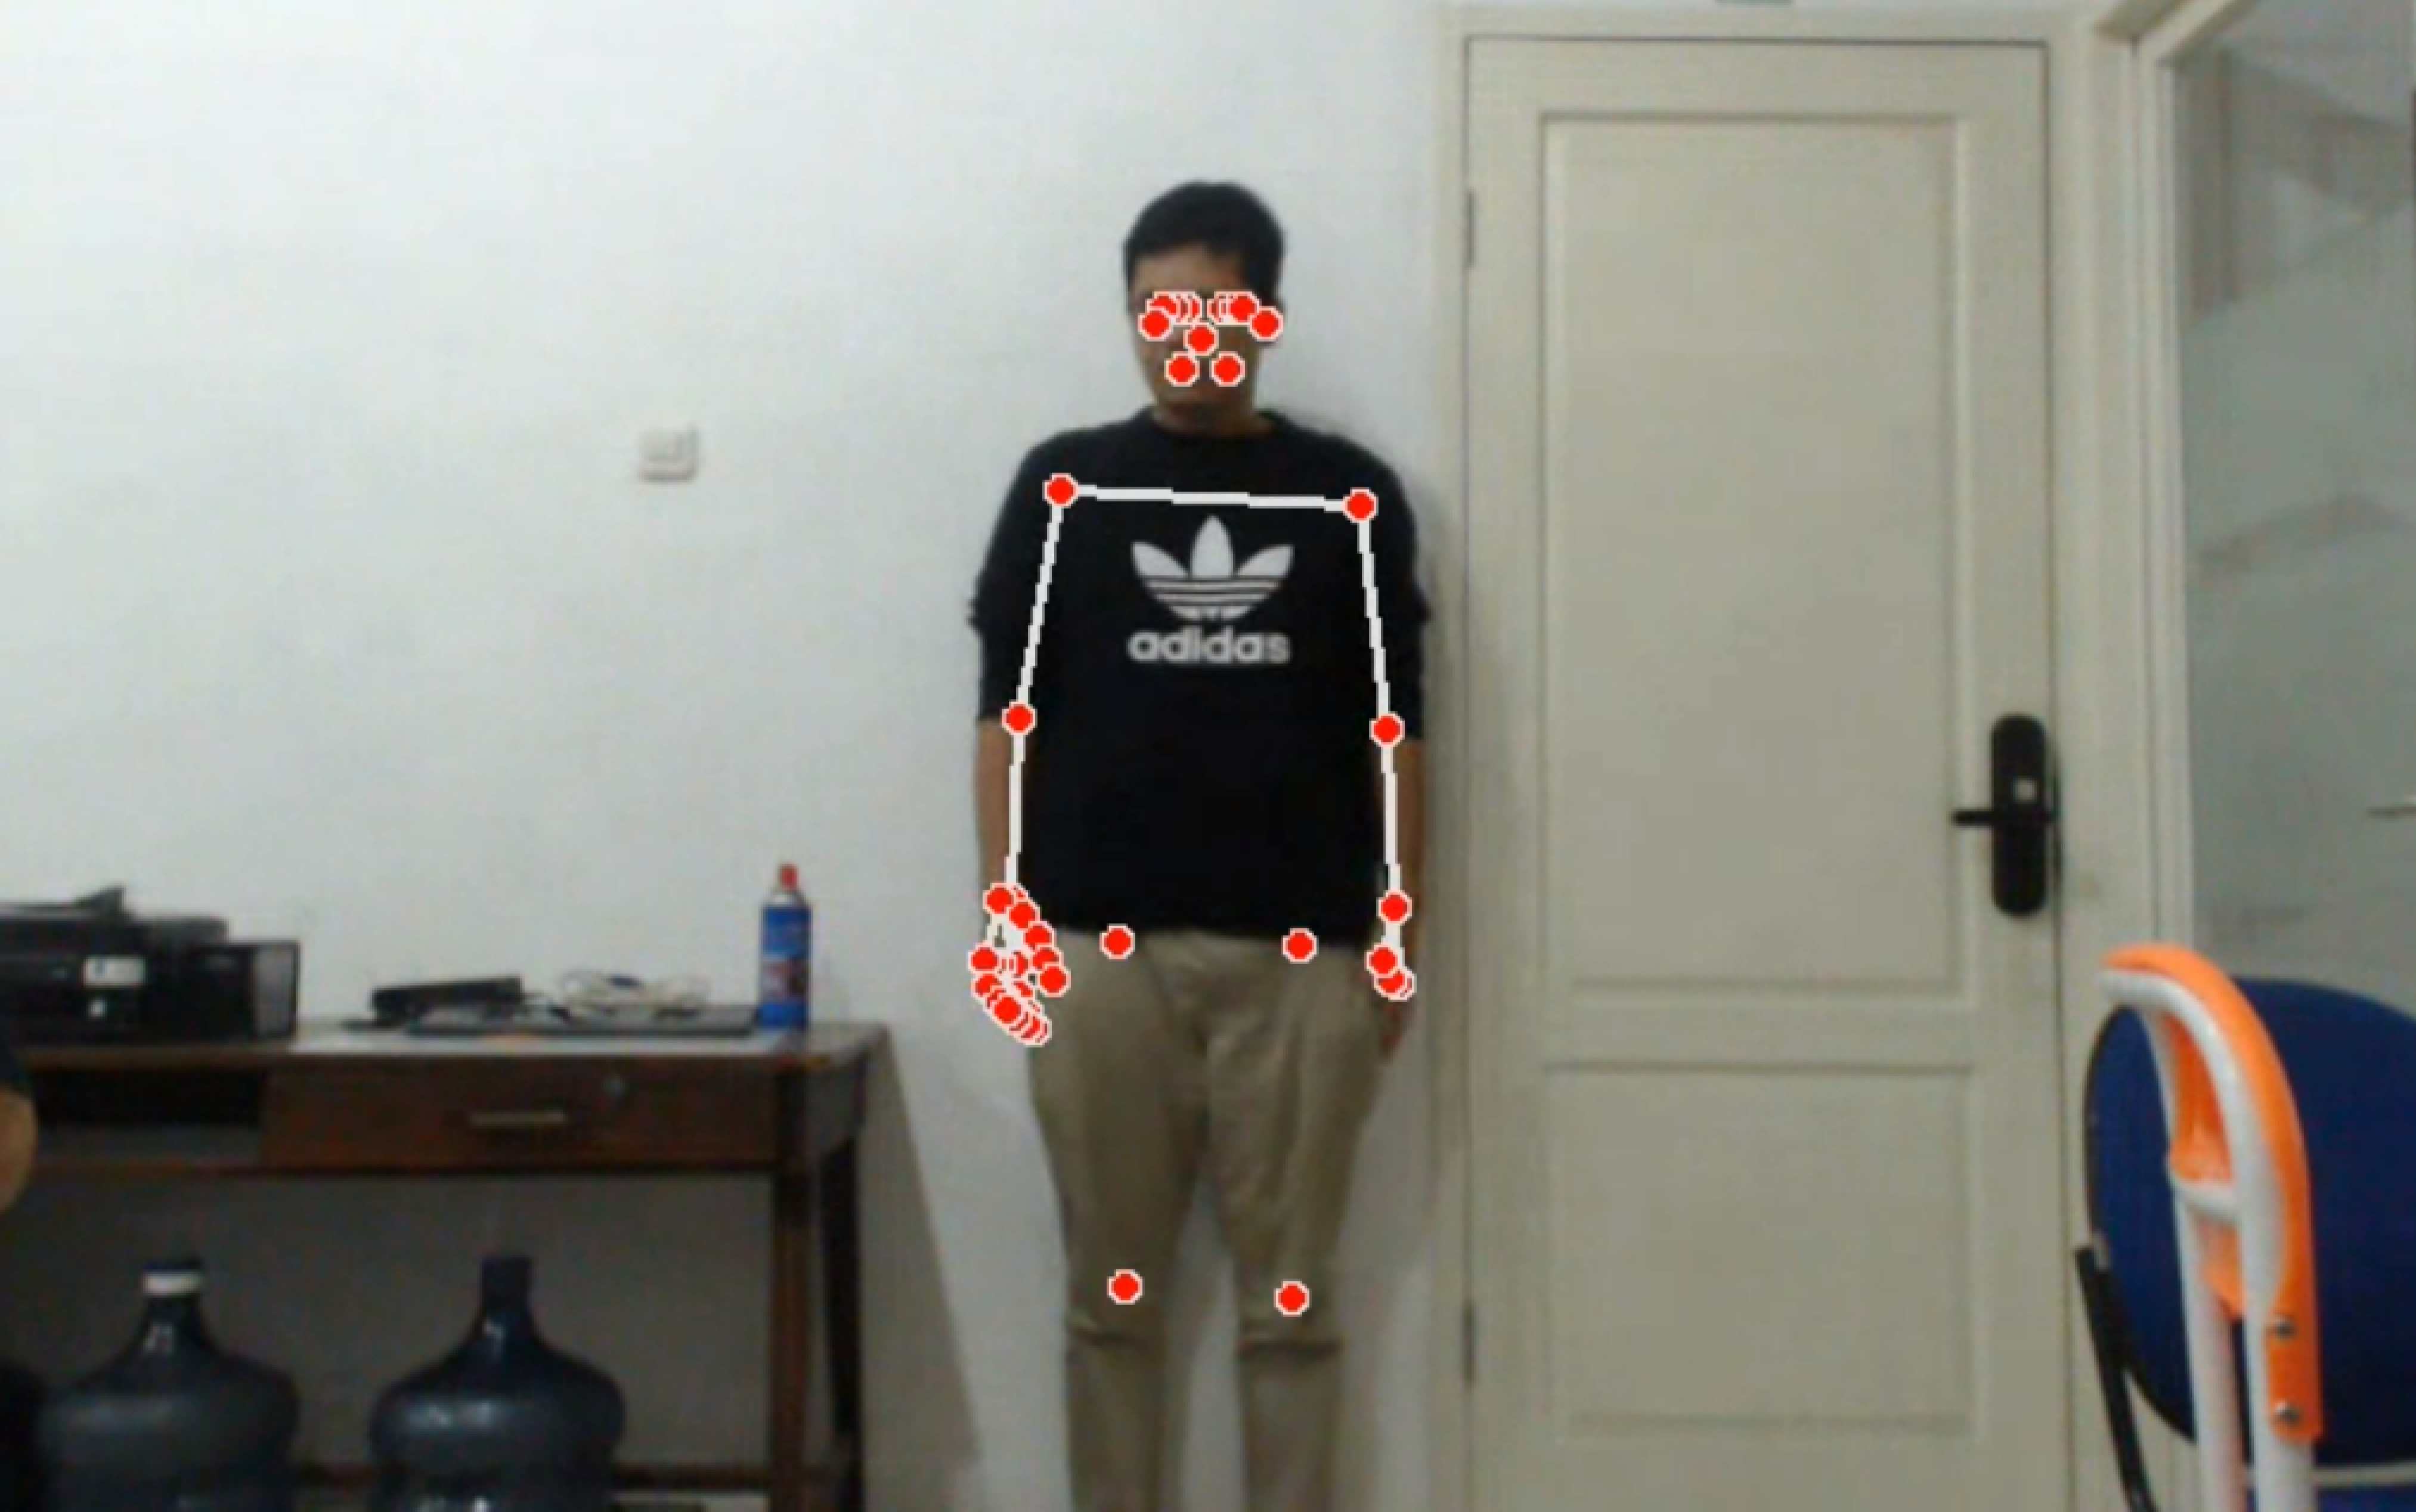
\includegraphics[scale=0.3]{gambar/bab4-evan.png}                 \\
  \hline
\end{longtable}

Pada pengujian dengan menggunakan subjek yang berbeda ini dilakukan untuk memahami bagaimana performa model pada pengguna selain darii penulis. Hal ini dilakukan demi melihat apakah model berhasil beradaptasi terhadap data yang bukan merupakan dataset yang digunakan dalam \emph{training} sehingga kedepannya dapat digunakan oleh kalangan luas. Adapun subjek yang akan diujikan berjumlah 2, yaitu 1 perempuan dan 1 laki - laki. Adapun gambaran subjek yang akan diujikan dapat dilihat pada tabel \ref{tb:kondisisubjek}. 

Model penerjemah bahasa Indonesia (BISINDO) yang akan digunakan pada pengujian ini adalah model pada bagian \ref{sec:analisismodel3} karena merupakan model yang menghasilkan klasifikasi yang terbaik jika dibandingkan dengan model lainnya. Untuk setiap intensitas cahaya akan dilakukan pengujian sebanyak tiga kali dengan jarak terhadap kamera sebesar 300 cm dan intensitas cahaya yang berkisar pada nilai 125 lux atau kondisi ruangan terang. Pada setiap pengujian akan dicari hasil klasifikasi model, waktu yang dibutuhkan model untuk menghasilkan klasifikasi bahasa isyarat berdasarkan data koordinat yang diberikan(\emph{processing time}), waktu total yang dibutuhkan dalam menghasilkan klasifikasi bahasa isyarat (\emph{complete time}), dan rata - rata FPS (\emph{frame per second}) yang didapatkan ketika proses klasifikasi dilakukan pada website.  

\subsection{Pengujian Subjek Perempuan}
\label{sec:analisisperempuan}

\begin{longtable}{|c|c|c|c|c|}
  \caption{Pengujian Pertama Model di Subjek Berbeda Perempuan}
  \label{tb:prediksiperempuan1}                                   \\
  \hline
  \rowcolor[HTML]{C0C0C0}
  \textbf{Kosakata} & \textbf{Klasifikasi Model} & \textbf{\emph{Processing Time}} & \textbf{\emph{Complete Time}} & \textbf{\emph{FPS}}\\
  \hline
  Maaf              & \textcolor{red}{Tolong}       & 0.09316 detik                           & 3.20865 detik                                  & 9.349722025\\
  Tolong            & Tolong                        & 0.09346 detik                           & 2.87486 detik                                  & 10.43527934\\
  Nama              & Nama                          & 0.09218 detik                           & 3.25495 detik                                  & 9.216731308\\
  Saya              & Saya                          & 0.09530 detik                           & 3.12871 detik                                  & 9.588624336\\
  Siapa             & Siapa                         & 0.09518 detik                           & 2.93024 detik                                  & 10.23807536\\
  Rumah             & \textcolor{red}{Delete}       & 0.10196 detik                           & 3.01911 detik                                  & 9.936707241\\
  Delete            & Delete                        & 0.10392 detik                           & 3.05715 detik                                  & 9.813073792\\
  Standby           & Standby                       & 0.09530 detik                           & 1.47974 detik                                  & 20.27379727\\
  Translate         & Translate                     & 0.09317 detik                           & 2.94322 detik                                  & 10.19291748\\
  \hline
\end{longtable}



\begin{longtable}{|c|c|c|c|c|}
  \caption{Pengujian Kedua Model di Subjek Berbeda Perempuan}
  \label{tb:prediksiperempuan2}                                   \\
  \hline
  \rowcolor[HTML]{C0C0C0}
  \textbf{Kosakata} & \textbf{Klasifikasi Model} & \textbf{\emph{Processing Time}} & \textbf{\emph{Complete Time}} & \textbf{\emph{FPS}}\\
  \hline
  Maaf              & Maaf                          & 0.09658 detik                           & 3.10876 detik                                  & 9.650153232\\
  Tolong            & Tolong                        & 0.09834 detik                           & 2.89284 detik                                  & 10.37041506\\
  Nama              & Nama                          & 0.09465 detik                           & 2.98028 detik                                  & 10.06617659\\
  Saya              & Saya                          & 0.09416 detik                           & 2.92525 detik                                  & 10.2555235\\
  Siapa             & Siapa                         & 0.09781 detik                           & 2.92773 detik                                  & 10.24682955\\
  Rumah             & Rumah                         & 0.09567 detik                           & 3.06411 detik                                  & 9.790762709\\
  Delete            & Delete                        & 0.10792 detik                           & 3.37185 detik                                  & 8.897189125\\
  Standby           & Standby                       & 0.09644 detik                           & 1.53859 detik                                  & 19.49841476\\
  Translate         & Translate                     & 0.10363 detik                           & 2.96890 detik                                  & 10.10473568\\
  \hline
\end{longtable}



\begin{longtable}{|c|c|c|c|c|}
  \caption{Pengujian Ketiga Model di Subjek Berbeda Perempuan}
  \label{tb:prediksiperempuan3}                                   \\
  \hline
  \rowcolor[HTML]{C0C0C0}
  \textbf{Kosakata} & \textbf{Klasifikasi Model} & \textbf{\emph{Processing Time}} & \textbf{\emph{Complete Time}} & \textbf{\emph{FPS}}\\
  \hline
  Maaf              & Maaf                          & 0.09668 detik                           & 3.10362 detik                                  & 9.666143525\\
  Tolong            & Tolong                        & 0.09738 detik                           & 3.04991 detik                                  & 9.836340227\\
  Nama              & Nama                          & 0.09641 detik                           & 2.92788 detik                                  & 10.24632891\\
  Saya              & Saya                          & 0.09479 detik                           & 1.46574 detik                                  & 20.46750762\\
  Siapa             & Siapa                         & 0.09821 detik                           & 3.08167 detik                                  & 9.734997029\\
  Rumah             & Rumah                         & 0.09820 detik                           & 2.87077 detik                                  & 10.45015111\\
  Delete            & Delete                        & 0.11417 detik                           & 3.02126 detik                                  & 9.929626447\\
  Standby           & Standby                       & 0.09473 detik                           & 1.54900 detik                                  & 19.36732451\\
  Translate         & Translate                     & 0.09833 detik                           & 3.12762 detik                                  & 9.591957427\\
  \hline
\end{longtable}



Berdasarkan tiga pengujian yang telah dilakukan, didapatkan bahwa hampir keseluruhan klasifikasi model yang sesuai dengan \emph{class} kosakata. Namun, terdapat beberapa kesalahan model dalam melakukan klasifikasi. Dapat dilihat pada tabel \ref{tb:prediksiperempuan1} untuk isyarat kosakata "Maaf" diklasifikasikan sebagai "Tolong". Hal ini dapat disebabkan oleh kesalahan pola gerakan isyarat yang digunakan, dimana kurang ditekankannya keunikan atau \emph{feature} dari masing - masing gerakan bahasa isyarat.  Secara garis besar, hasil pengujian ini menunjukkan bahwa model dengan mudah dapat mengklasifikasikan bahasa isyarat yang diperagakan oleh pengguna dengan jenis kelamin perempuan dengan akurasi sebesar 92.5\%. 

Apabila dilihat berdasarkan waktu pemrosesan, rata - rata waktu yang dibutuhkan model untuk menghasilkan klasifikasi bahasa isyarat (\emph{processing time}) adalah 0.098 detik dan rata - rata waktu yang dibutuhkan dalam menghasilkan klasifikasi bahasa isyarat (\emph{complete time}) adalah 2.810 detik. Hal ini menunjukkan bahwa pada subjek perempuan yang berbeda dengan penulis tidak mempengaruhi nilai \emph{processing time} dan \emph{complete time}. Adapun rata - rata nilai FPS yang didapatkan berdasarkan pengujian yang dilakukan bernilai 11.378. Nilai menunjukkan bahwa subjek perempuan yang berbeda dengan penulis tidak berpengaruh secara signifikan terhadap sistem yang ada. Hal ini juga menguatkan bahwa model telah dapat beradaptasi dengan subjek yang berbeda dengan penulis.

\subsection{Pengujian Subjek Laki - Laki}
\label{sec:analisislaki}

\begin{longtable}{|c|c|c|c|c|}
  \caption{Pengujian Pertama Model di Subjek Berbeda Laki - Laki}
  \label{tb:prediksilaki1}                                   \\
  \hline
  \rowcolor[HTML]{C0C0C0}
  \textbf{Kosakata} & \textbf{Klasifikasi Model} & \textbf{\emph{Processing Time}} & \textbf{\emph{Complete Time}} & \textbf{\emph{FPS}}\\
  \hline
  Maaf              & \textcolor{red}{Tolong}       & 0.10172 detik                           & 3.06706 detik                                  & 9.781355671\\
  Tolong            & Tolong                        & 0.09743 detik                           & 3.01787 detik                                  & 9.940781506\\
  Nama              & Nama                          & 0.09616 detik                           & 3.03984 detik                                  & 9.868927367\\
  Saya              & Saya                          & 0.10311 detik                           & 1.46807 detik                                  & 20.4349991\\
  Siapa             & Siapa                         & 0.10661 detik                           & 2.92250 detik                                  & 10.2651868\\
  Rumah             & \textcolor{red}{Delete}       & 0.08927 detik                           & 2.82929 detik                                  & 10.60335116\\
  Delete            & Delete                        & 0.09602 detik                           & 3.15976 detik                                  & 9.494380522\\
  Standby           & Standby                       & 0.09914 detik                           & 1.53859 detik                                  & 19.49841476\\
  Translate         & Translate                     & 0.10099 detik                           & 2.91128 detik                                  & 10.30475694\\
  \hline
\end{longtable}


\begin{longtable}{|c|c|c|c|c|}
  \caption{Pengujian Kedua Model di Subjek Berbeda Laki - Laki}
  \label{tb:prediksilaki2}                                   \\
  \hline
  \rowcolor[HTML]{C0C0C0}
  \textbf{Kosakata} & \textbf{Klasifikasi Model} & \textbf{\emph{Processing Time}} & \textbf{\emph{Complete Time}} & \textbf{\emph{FPS}}\\
  \hline
  Maaf              & Maaf                          & 0.10625 detik                           & 2.97540 detik                                  & 10.08267967\\
  Tolong            & Tolong                        & 0.09605 detik                           & 2.98787 detik                                  & 10.04060957\\
  Nama              & Nama                          & 0.09938 detik                           & 2.85504 detik                                  & 10.50772114\\
  Saya              & Saya                          & 0.09951 detik                           & 1.54736 detik                                  & 19.38782548\\
  Siapa             & Siapa                         & 0.08863 detik                           & 2.88129 detik                                  & 10.41199104\\
  Rumah             & Rumah                         & 0.08927 detik                           & 2.87948 detik                                  & 10.41856029\\
  Delete            & Delete                        & 0.09708 detik                           & 3.09736 detik                                  & 9.685652464\\
  Standby           & Standby                       & 0.10267 detik                           & 1.54900 detik                                  & 19.36732451\\
  Translate         & Translate                     & 0.10302 detik                           & 3.11868 detik                                  & 9.619455854\\
  \hline
\end{longtable}


\newpage
\begin{longtable}{|c|c|c|c|c|}
  \caption{Pengujian Ketiga Model di Subjek Berbeda Laki - Laki}
  \label{tb:prediksilaki3}                                   \\
  \hline
  \rowcolor[HTML]{C0C0C0}
  \textbf{Kosakata} & \textbf{Klasifikasi Model} & \textbf{\emph{Processing Time}} & \textbf{\emph{Complete Time}} & \textbf{\emph{FPS}}\\
  \hline
  Maaf              & Maaf                          & 0.09524 detik                           & 3.01198 detik                                  & 9.960233196\\
  Tolong            & Tolong                        & 0.10116 detik                           & 3.02593 detik                                  & 9.914323197\\
  Nama              & Nama                          & 0.10365 detik                           & 2.99661 detik                                  & 10.01129949\\
  Saya              & Saya                          & 0.09723 detik                           & 1.47242 detik                                  & 20.37464478\\
  Siapa             & Siapa                         & 0.09995 detik                           & 2.96723 detik                                  & 10.11043536\\
  Rumah             & Rumah                         & 0.08927 detik                           & 2.96376 detik                                  & 10.12226931\\
  Delete            & Delete                        & 0.09006 detik                           & 2.90455 detik                                  & 10.32863563\\
  Standby           & Standby                       & 0.10000 detik                           & 2.02851 detik                                  & 14.78919346\\
  Translate         & Translate                     & 0.10083 detik                           & 3.19591 detik                                  & 9.387010429\\
  \hline
\end{longtable}



Berdasarkan tiga pengujian yang telah dilakukan, didapatkan bahwa hampir keseluruhan klasifikasi model yang sesuai dengan \emph{class} kosakata. Namun, terdapat beberapa kesalahan model dalam melakukan klasifikasi. Dapat dilihat pada tabel \ref{tb:prediksilaki1} untuk kosakata isyarat "Maaf" diklasifikasikan sebagai "Tolong". Hal ini dapat disebabkan oleh kesalahan pola gerakan isyarat yang digunakan, dimana kurang ditekankannya keunikan atau \emph{feature} dari masing - masing gerakan bahasa isyarat.  Secara garis besar, hasil pengujian ini menunjukkan bahwa model dengan mudah dapat mengklasifikasikan bahasa isyarat yang diperagakan oleh pengguna dengan jenis kelamin perempuan dengan akurasi sebesar 92.5\%. 

Apabila dilihat berdasarkan waktu pemrosesan, rata - rata waktu yang dibutuhkan model untuk menghasilkan klasifikasi bahasa isyarat (\emph{processing time}) adalah 0.098 detik dan rata - rata waktu yang dibutuhkan dalam menghasilkan klasifikasi bahasa isyarat (\emph{complete time}) adalah 2.682 detik. Hal ini menunjukkan bahwa pada subjek yang berbeda dengan penulis tidak mempengaruhi \emph{processing time} dan \emph{complete time}. Adapun berdasarkan 3 pengujian yang dilakukan, didapatkan rata - rata nilai FPS bernilai 12.026. Hal ini menunjukkan bahwa perbedaan subjek tidak berpengaruh secara signifikan terhadap kinerja sistem yang ada. Data ini juga menunjukkan bahwa proses normalisasi yang dilakukan telah berhasil dan memudahkan model untuk mengklasifikasikan gerakan bahasa isyarat secara \emph{general} atau menyeluruh.  

\subsection{Rangkuman Pengujian Subjek Berbeda}
\label{sec:analisissubjekberbeda}

\begin{longtable}{|c|c|c|c|c|}
  \caption{Rangkuman Pengujian Subjek Berbeda}
  \label{tb:evaluasiSubjek}                                   \\
  \hline
  \rowcolor[HTML]{C0C0C0}
  \textbf{Subjek} & \textbf{Akurasi} & \emph{\textbf{Avg. Processing Time}} & \emph{\textbf{Avg. Complete Time}} & \textbf{FPS} \\
  \hline
  Perempuan & 0.93   & 0.0988 detik & 2.6636 detik & 12.026  \\
  Laki - Laki & 0.93 & 0.0973 detik & 2.8191 detik & 11.378 \\
  \hline
\end{longtable}

Secara keseluruhan, dapat dilihat bahwa model dapat bekerja untuk melakukan klasifikasi berdasarkan gerakan isyarat dari subjek yang berbeda dengan penulis. Normalisasi data yang dilakukan telah berhasil menggeneralisasi data sehingga model dapat menghasilkan klasifikasi yang baik meskipun berasal dari subjek yang berbeda dari penulis. Hal ini dibuktikan dengan akurasi pada subjek laki - laki dan perempuan bernilai 0.93 atau 93\%. Adapun nilai dari \emph{average processing time} dan \emph{average complete time} berkisar pada 0.09 detik dan 2.6 detik. Data ini tidak jauh berbeda dengan bebrapa pengujian sebelumnya yang telah dilakukan oleh penulis dan menunjukkan bahwa proses normalisasi yang dilakukan telah berhasil menghasilkan model yang memiliki kemampuan untuk beradaptasi terhadap posisi dan terhadap skala pengguna.

\section{Pengujian Pembentukan Kalimat dan Konversi Suara}
\label{sec:analisiskalimat}

Pada pengujian pembentukan kalimat dan konversi suara ini dilakukan untuk memahami bagaimana sistem penerjemah bahasa isyarat Indonesia (BISINDO) jika digunakan untuk membentuk kalimat dan melakukan konversi suara berdasarkan kalimat yang dibentuk. Adapun sistematika dalam pembentukan kalimat dan konversi ini mengacu dengan \emph{flowchart} yang telah dijelaskan pada sub bab \ref{sec:metodologisistemkontrol}. Kombinasi kata untuk membentuk kalimat pada sistem ini dapat dilihat pada tabel \ref{tb:kalimatpengujian}. Perlu diperhatikan bahwa untuk mendeteksi kosakata dan mengontrol sistem (\emph{translate} dan \emph{delete}) memerlukan pengguna untuk berada di keadaan \emph{standby} terlebih dahulu. Pembentukan kalimat dan konveri suara pada pengujian ini dilakukan secara sekuensial dengan memastikan bahwa setiap kosakata benar terklasifikasi. Kemudian, kalimat akan diterjemahkan dengan melakukan gerakan isyarat kontrol "\emph{translate}" dan diakhiri dengan melakukan gerakan isyarat kontrol "\emph{delete}" untuk memastikan bahwa kosakata terakhir berhasil dihapus. Pengulangan bahasa isyarat dilakukan maksimal sebanyak tiga kali.

\begin{longtable}{|c|c|}
  \caption{Kalimat Pengujian}
  \label{tb:kalimatpengujian}                                   \\
  \hline
  \rowcolor[HTML]{C0C0C0}
  \textbf{Kombinasi Kosakata} & \textbf{Kalimat Akhir}  \\
  \hline
  "Maaf" + "Siapa" + "Nama"            &  "Maaf siapa nama kamu?"               \\

  "Maaf" + "Tolong "+ "Saya"            & "Maaf tolong bantu saya"                 \\
  
  "Maaf" + "Rumah" + "Siapa"            & "Maaf ini rumah siapa?"                 \\

  "Rumah" + "Saya"            & "Ini rumah saya"                 \\

  "Rumah" + "Siapa"            & "Ini rumah siapa"                 \\

  "Siapa" + "Nama"            & "Siapa nama kamu?"                 \\

  "Tolong" + "Saya"            & "Tolong bantu saya"                 \\
  \hline
\end{longtable}

Model penerjemah bahasa Indonesia (BISINDO) yang akan digunakan pada pengujian ini adalah model pada bagian \ref{sec:analisismodel3} karena merupakan model yang menghasilkan klasifikasi yang terbaik jika dibandingkan dengan model lainnya. Untuk setiap kombinasi kalimat akan dilakukan pengujian sebanyak satu kali dengan kondisi ruangan yang memiliki intensitas cahaya yang terang (berkisar pada 125 lux) dan jarak kamera dengan pengguna bernilai 300 cm. Pada setiap kombinasi kalimat akan dicari hasil klasifikasi model, waktu yang dibutuhkan model untuk menghasilkan klasifikasi bahasa isyarat berdasarkan data koordinat yang diberikan(\emph{processing time}), waktu total yang dibutuhkan dalam menghasilkan klasifikasi bahasa isyarat (\emph{complete time}), dan rata - rata FPS (\emph{frame per second}) yang didapatkan ketika proses klasifikasi dilakukan pada website.  

\begin{longtable}{|c|c|c|c|c|}
  \caption{Pengujian Pembentukan Kalimat Pertama}
  \label{tb:prediksikombinasi1}                                   \\
  \hline
  \rowcolor[HTML]{C0C0C0}
  \textbf{Kosakata} & \textbf{Klasifikasi Model} & \textbf{\emph{Processing Time}} & \textbf{\emph{Complete Time}} & \textbf{\emph{FPS}}\\
  \hline
  Maaf                & Maaf                          & 0.09733 detik                           & 3.10390 detik                                  & 9.665252548\\
  Siapa               & Siapa                         & 0.09816 detik                           & 2.81724 detik                                  & 10.64871191\\
  Nama                & Nama                          & 0.09517 detik                           & 3.09707 detik                                  & 9.686569577\\
  Delete              & Delete                        & 0.09404 detik                           & 3.14265 detik                                  & 9.546068848\\
  Translate           & Translate                     & 0.09449 detik                           & 2.94607 detik                                  & 10.18304357\\
  \hline
\end{longtable}



\begin{longtable}{|c|c|c|c|c|}
  \caption{Pengujian Pembentukan Kalimat Kedua}
  \label{tb:prediksikombinasi2}                                   \\
  \hline
  \rowcolor[HTML]{C0C0C0}
  \textbf{Kosakata} & \textbf{Klasifikasi Model} & \textbf{\emph{Processing Time}} & \textbf{\emph{Complete Time}} & \textbf{\emph{FPS}}\\
  \hline
  Maaf              & Maaf                          & 0.10064 detik                           & 2.82230 detik                                  & 10.62963207\\
  Tolong            & Tolong                        & 0.09766 detik                           & 2.84455 detik                                  & 10.54648137\\
  Saya              & Nama                          & 0.09680 detik                           & 2.91340 detik                                  & 10.29724322\\
  Delete            & Delete                        & 0.09554 detik                           & 3.14218 detik                                  & 9.54750301\\
  Translate         & Translate                     & 0.09473 detik                           & 2.88474 detik                                  & 10.39954775\\
  \hline
\end{longtable}



\begin{longtable}{|c|c|c|c|c|}
  \caption{Pengujian Pembentukan Kalimat Ketiga}
  \label{tb:prediksikombinasi3}                                   \\
  \hline
  \rowcolor[HTML]{C0C0C0}
  \textbf{Kosakata} & \textbf{Klasifikasi Model} & \textbf{\emph{Processing Time}} & \textbf{\emph{Complete Time}} & \textbf{\emph{FPS}}\\
  \hline
  Maaf              & Maaf                          & 0.10551 detik                           & 2.96949 detik                                  & 10.10273987\\
  Rumah             & Tolong                        & 0.09711 detik                           & 2.98955 detik                                  & 10.03494031\\
  Siapa             & Nama                          & 0.10716 detik                           & 2.91791 detik                                  & 10.28134123\\
  Delete            & Delete                        & 0.09795 detik                           & 2.98041 detik                                  & 10.0657176\\
  Translate         & Translate                     & 0.10163 detik                           & 2.95819 detik                                  & 10.14133491\\
  \hline
\end{longtable}


\begin{longtable}{|c|c|c|c|c|}
  \caption{Pengujian Pembentukan Kalimat Keempat}
  \label{tb:prediksikombinasi4}                                   \\
  \hline
  \rowcolor[HTML]{C0C0C0}
  \textbf{Kosakata} & \textbf{Klasifikasi Model} & \textbf{\emph{Processing Time}} & \textbf{\emph{Complete Time}} & \textbf{\emph{FPS}}\\
  \hline
  Rumah             & \textcolor{red}{Delete}       & 0.09740 detik                           & 3.04230 detik                                  & 9.86094582\\
  Saya              & Saya                          & 0.09879 detik                           & 1.49619 detik                                  & 20.05088368\\
  Delete            & Delete                        & 0.09497 detik                           & 2.90618 detik                                  & 10.32281438\\
  Translate         & Translate                     & 0.10316 detik                           & 2.94376 detik                                  & 10.19103526\\
  \hline
\end{longtable}



\begin{longtable}{|c|c|c|c|c|}
  \caption{Pengujian Pembentukan Kalimat Kelima}
  \label{tb:prediksikombinasi5}                                   \\
  \hline
  \rowcolor[HTML]{C0C0C0}
  \textbf{Kosakata} & \textbf{Klasifikasi Model} & \textbf{\emph{Processing Time}} & \textbf{\emph{Complete Time}} & \textbf{\emph{FPS}}\\
  \hline
  Rumah             & Rumah                          & 0.09345 detik                           & 1.56138 detik                                  & 19.21375007\\
  Siapa             & Siapa                          & 0.09489 detik                           & 1.45863 detik                                  & 20.5672703\\
  Delete            & Delete                         & 0.09873 detik                           & 3.03389 detik                                  & 9.888308406\\
  Translate         & Translate                      & 0.10570 detik                           & 2.90638 detik                                  & 10.32210306\\
  \hline
\end{longtable}



\begin{longtable}{|c|c|c|c|c|}
  \caption{Pengujian Pembentukan Kalimat Keenam}
  \label{tb:prediksikombinasi6}                                   \\
  \hline
  \rowcolor[HTML]{C0C0C0}
  \textbf{Kosakata} & \textbf{Klasifikasi Model} & \textbf{\emph{Processing Time}} & \textbf{\emph{Complete Time}} & \textbf{\emph{FPS}}\\
  \hline
  Siapa             & Siapa                          & 0.10315 detik                           & 3.04230 detik                                  & 20.34706847\\
  Nama              & Nama                           & 0.09985 detik                           & 1.49619 detik                                  & 21.00081614\\
  Delete            & Delete                         & 0.09890 detik                           & 2.90618 detik                                  & 10.29178557\\
  Translate         & Translate                      & 0.10316 detik                           & 2.94376 detik                                  & 10.06963244\\
  \hline
\end{longtable}


\newpage
\begin{longtable}{|c|c|c|c|c|}
  \caption{Pengujian Pembentukan Kalimat Ketujuh}
  \label{tb:prediksikombinasi7}                                   \\
  \hline
  \rowcolor[HTML]{C0C0C0}
  \textbf{Kosakata} & \textbf{Klasifikasi Model} & \textbf{\emph{Processing Time}} & \textbf{\emph{Complete Time}} & \textbf{\emph{FPS}}\\
  \hline
  Tolong             & Tolong                         & 0.10104 detik                           & 3.00838 detik                                  & 9.972144688\\
  Saya               & Saya                           & 0.10042 detik                           & 2.94446 detik                                  & 10.18863396\\
  Delete             & Delete                         & 0.09524 detik                           & 3.03605 detik                                  & 9.881249838\\
  Translate          & Translate                      & 0.10302 detik                           & 3.01550 detik                                  & 9.948586094\\
  \hline
\end{longtable}


% \begin{longtable}{|c|c|}
%   \caption{Waktu \emph{Translate} Kombinasi Kalimat}
%   \label{tb:waktutranslate}                                   \\
%   \hline
%   \rowcolor[HTML]{C0C0C0}
%   \textbf{Kalimat} & \textbf{Waktu Penyuaraan Kalimat}\\
%   \hline
%   Maaf siapa nama kamu?              & 1.9165489673614502                               \\
%   Maaf tolong bantu saya            & 1.824713945388794                            \\
%   Maaf ini rumah siapa?              & 1.9595482349395752                         \\
%   Ini rumah saya              & 1.5204029083251953                             \\
%   Ini rumah siapa?              & 1.605020523071289                             \\
%   Siapa nama kamu?              & 1.606485366821289                             \\
%   Tolong bantu saya              & 1.5231249332427979                             \\
%   \hline
% \end{longtable}

Untuk kalimat yang terdiri dari kombinasi tiga kosakata, yaitu kalimat pertama, kalimat kedua, dan kalimat ketiga telah berhasil dibentuk. Hal ini dapat dilihat dari untuk kombinasi kosakata pembentuk kalimat tersebut telah berhasil diklasifikasikan dengan akurasi sebesar 100\% (dapat dilihat pada tabel \ref{tb:prediksikombinasi1}, tabel \ref{tb:prediksikombinasi2}, dan tabel \ref{tb:prediksikombinasi3}). Pada kalimat pertama, rata - rata \emph{processing time} bernilai 0.096 detik dan \emph{complete time} bernilai 3.021 detik. Pada kalimat kedua, rata - rata \emph{processing time} bernilai 0.097 detik dan \emph{complete time} bernilai 2.921 detik. Pada kalimat ketiga, rata - rata \emph{processing time} bernilai 0.102 detik dan \emph{complete time} bernilai 2.963 detik. Adapun berdasarkan 3 pengujian yang dilakukan, didapat bahwa rata - rata nilai FPS bernilai 10.1184. Dapat dilihat bahwa meskipun gerakan bahasa isyarat dilakukan secara sekuensial, tetap dapat menghasilkan klasifikasi akurasi yang baik. 

Untuk kalimat yang terdiri dari kombinasi dua kosakata, yaitu kalimat kelima, keenam, dan ketujuh telah berhasil dibentuk. Hal ini dapat dilihat dari kombinasi kosakata pembentuk kalimat tersebut telah berhasil diklasifikasikan dengan akurasi sebesar 93.75\% (dapat dilihat pada tabel \ref{tb:prediksikombinasi5}, \ref{tb:prediksikombinasi6}, \ref{tb:prediksikombinasi7}). Pada kalimat kelima, rata - rata \emph{processing time} bernilai 0.098 detik dan \emph{complete time} bernilai 2.240 detik. Pada kalimat keenam, rata - rata \emph{processing time} bernilai 0.100 detik dan \emph{complete time} bernilai 2.199 detik.Pada kalimat ketujuh, rata - rata \emph{processing time} bernilai 0.100 detik dan \emph{complete time} bernilai 3.001 detik. Dapat dilihat bahwa untuk \emph{complete time} relatif lebih cepat pada kalimat dengan kombinasi tiga kosakata jika dibandingkan dengan kalimat dengan kombinasi dua kosakata. Adapun berdasarkan 3 pengujian yang dilakukan, didapat bahwa rata - rata nilai FPS bernilai 13.2573. Apabila dibandingkan dengan kalimat yang dibentuk dari 3 kosakata, terdapat peningkatan FPS yang cukup signifikan yang dapat disebabkan oleh beban sistem yang lebih berat seiring dengan banyaknya kosakata yang dibentuk pada pengujian yang dilakukan secara sekuensial ini. 

Namun, pada kalimat keempat ("Ini rumah saya") terdapat kosakata yang salah sehingga menyebabkan gagalnya terbentuk kalimat tersebut dalam pengujian yang dilakukan secara sekue\\nsial. Isyarat kosakata "Rumah" diklasifikasikan sebagai "Delete". Hal ini dapat disebabkan oleh adanya kemiripan gerakan antara kedua kosakata tersebut. rata - rata \emph{processing time} bernilai 0.099 detik dan \emph{complete time} bernilai 2.597 detik.

\subsection{Rangkuman Pengujian Pembentukan Kalimat dan Konveri Suara}
\label{sec:analisikalimatsuara}

\begin{longtable}{|c|c|c|c|c|}
  \caption{Rangkuman Pengujian Pembentukan Kalimat dan Konveri Suara}
  \label{tb:evaluasiKalimatdanSuara}                                   \\
  \hline
  \rowcolor[HTML]{C0C0C0}
  \textbf{Kosakata} & \textbf{Akurasi} & \emph{\textbf{Avg. Processing Time}} & \emph{\textbf{Avg. Complete Time}} & \textbf{FPS}\\
  \hline
  2 kosakata & 1.00 & 0.0993 detik & 2.8303 detik & 13.2573  \\
  3 kosakata & 0.93 & 0.0981 detik & 2.0513 detik & 10.1184  \\
  \hline
\end{longtable}

Secara keseluruhan, dapat dilihat bahwa sistem penerjemah dapat melakukan klasifikasi dengan baik dalam menerjemahkan gerakan isyarat yang dilakukan secara sekuensial. Hal ini tidak berdampak secara signifikan terhadap \emph{average processing time} dan \emph{average complete time}. Akurasi klasifikasi masih sangat baik, dimana pada kalimat dengan 2 kosakata bernilai 1.00 atau 100\% dan 3 kosakata bernilai 0.93 atau 93\%. Pada kalimat dengan 3 kosakata, hanya 1 kalimat yang tidak berhasil untuk dibentuk, yaitu kalimat "Ini rumah saya". Library gtts (Google Text-To-Speech) telah dapat berfungsi dengan baik untuk menkonversi data teks dalam bentuk \emph{string} ke dalam suara sesuai dengan kalimat yang ditandai dengan gerakan isyarat \emph{translate} yang berhasil dideteksi pada setiap percobaan. Adapun secara keseluruhan, tingkat keberhasilan sistem penerjemah dalam membentuk kalimat adalah sebesar 85.7\%. Adapun pada rata - rata FPS yang dihasilkan meningkat pada kalimat yang dibentuk dari 2 kosakata jika dibandingkan dengan kaliamt yang dibentuk dari 3 kosakata. Hal ini menunjukkan bahwa seiring dengan meningkatnya koskata yang dibentuk secara sekuensial menghasilkan beban kerja sistem yang lebih berat, namun tidak mempengaruhi secara signifikan hasil klasifikasi gerakan isyarat yang ada.

% Untuk kalimat yang terdiri dari kombinasi tiga kosakata, pada kombinasi kalimat pertama didapat bahwa keseluruhan kosakata bahasa isyarat untuk kalimat "Maaf siapa nama kamu?" telah berhasil dibentuk. Hal ini dapat dilihat untuk seluruh kombinasi kosakata yang telah berhasil diklasifikasikan dengan akurasi sebesar 100\%. Untuk rata - rata \emph{processing time} dan \emph{complete time} adalah 0.096 detik  dan 3.021 detik. Pada kombinasi kalimat kedua, keseluruhan kosakata bahasa isyarat untuk kalimat "Maaf tolong bantu saya?" telah berhasil dibentuk. Hal ini dapat dilihat untuk seluruh kombinasi kosakata yang telah berhasil diklasifikasikan dengan akurasi sebesar 100\%. Untuk rata - rata \emph{processing time} dan \emph{complete time} adalah 0.097 detik  dan 2.921 detik. Pada kombinasi kalimat ketiga, keseluruhan kosakata bahasa isyarat untuk kalimat "Maaf ini rumah siapa?" telah berhasil dibentuk. Hal ini dapat dilihat untuk seluruh kombinasi kosakata yang telah berhasil diklasifikasikan dengan akurasi sebesar 100\%. Untuk rata - rata \emph{processing time} dan \emph{complete time} adalah 0.102 detik  dan 2.963 detik.

% Untuk kalimat yang terdiri dari kombinasi dua kosakata, pada kombinasi kalimat keempat didapat bahwa keseluruhan kosakata bahasa isyarat untuk kalimat "Ini rumah saya" tidak berhasil dibentuk. Hal ini disebabkan oleh kosakata "Rumah" diklasifikasikan sebagai "Delete". Untuk rata - rata \emph{processing time} dan \emph{complete time} adalah 0.096 detik dan 3.021 detik. Pada kombinasi kalimat keenam, keseluruhan bahasa isyarat untuk kalimat "Maaf tolong bantu saya"  telah berhasil dibentuk. Hal ini dapat dilihat untuk seluruh kombinasi kosakata telah berhasil diklasifikasikan dengan akurasi sebesar 100\%.  Untuk rata - rata \emph{processing time} dan \emph{complete time} adalah 0.098 detik  dan 2.240 detik.

% \section{Pengujian Performa NUC}
% \label{sec:analisisnuc}
% \section{Evaluasi Pengujian}
% \label{sec:analisispengujian}

% Dari pengujian yang \lipsum[1]

% % Contoh pembuatan tabel


% \lipsum[2-4]
